\chapter{Split-Quaternions as Dynamical Systems}
\label{chap:quaternion}
%\lsymb{$\vec{\alpha}$}{A differential form}

In this chapter, the geometric connection is made between the algebra of split-quaternions and the qualitative behavior of two-dimensional linear dynamical systems. 

\section{Split-quaternion algebra}
\subsection{Basic properties}
\label{ssec:quat_basics}
Like conventional quaternions, the split-quaternions form a number system that consists of linear combinations of four basis elements, which will be denoted by 1, \quati, \quatj and \quatk.\footnote
{Even though they behave similarly, the imaginary unit $\ii$ is not to be confused with the split-quaternion basis element \quati, because they belong to different number systems.}
The algebra of split-quaternions is associative but not commutative --- formally speaking, we are dealing with an algebraic structure called a \emph{noncommutative ring}. The multiplication table for the split-quaternion algebra is shown in \cref{tab:quat_table}. The set of split-quaternions is denoted by \spquaternions, since \quaternions is reserved for conventional quaternions.\footnote
{The `$\mathbb{H}$' is in honour of sir William Rowan Hamilton, who also developed the Hamiltonian formalism: the fruits of his work truly form the central theme in this thesis. \cite{Stillwell2008}}
\begin{table}[ht!]
    \centering
    \caption{Multiplication table for the split-quaternion algebra.}
    \label{tab:quat_table}
    \begin{tabular}{c|cccc}
        \toprule
        &         1      & \quati  & \quatj  & \quatk \\ 
        \midrule
        1       & 1      & \quati  & \quatj  & \quatk \\ 
        \quati  & \quati & -1      & \quatk  & -\quatj \\ 
        \quatj  & \quatj & -\quatk & 1       & -\quati \\ 
        \quatk  & \quatk & \quatj  & \quati  & 1 \\ 
        \bottomrule
    \end{tabular}
\end{table}

The important distinction from conventional quaternions resides in the diagonal elements of \cref{tab:quat_table}. For quaternions, all the nonreal basis elements square to $-1$, this is not the case for the split-quaternions (only \quati does). This is precisely the reason why split-quaternions are `split', for this difference in sign makes their norm (to be defined later) into an indefinite form. That is to say, whereas quaternions have a `metric signature' (in a very imprecise sense of the word metric) of $(+, +, +, +)$, for the split-quaternions we have $(+, +, -, -)$. The distinctive `metric' signature makes the algebra of split-quaternions  different from its conventional quaternion counterpart.

\paragraph{Dihedral group} The basis elements of the split-quaternions $\qty{1, \quati, \quatj, \quatk}$ form a finite group under multiplication, namely the \emph{dihedral group} \digroup{4}, which represents all the symmetries of a square: the identity, a 90-degree rotation and two reflections, as illustrated in \cref{fig:square_symmetry}. \cite{Dummit2004}
\begin{figure}[h!]
    \centering
    \begin{tikzpicture}
    \node[draw, inner sep=3mm,thick, fill=accent1!40] at (0, 0) {};
    \node[draw, inner sep=3mm,thick, fill=accent1!40] at (2, 0) {};
    \node[draw, inner sep=3mm,thick, fill=accent1!40] at (4, 0) {};
    \node[draw, inner sep=3mm,thick, fill=accent1!40] at (6, 0) {};
    \draw[->] (2, 0.7) arc (90:0:0.7);
    \draw[->] (2, -0.7) arc (270:180:0.7);
    \draw[dashdotted] (3.5, 0.5) -- (4.5, -0.5);
    \draw[<->] (3.75, -0.25) -- (4.25, 0.25);
    \draw[dashdotted] (5.5, -0.5) -- (6.5, 0.5);
    \draw[<->] (5.75, 0.25) -- (6.25, -0.25);
    \node[] at (0, -1.1) {1};
    \node[] at (2, -1.1) {\quati};
    \node[] at (4, -1.1) {\quatj};
    \node[] at (6, -1.1) {\quatk};

\end{tikzpicture}

    \caption{The dihedral group \digroup{4} is the symmetry group of a square. This group is isomorphic to the group formed by $1, \quati, \quatj$ and \quatk under multiplication.}
    \label{fig:square_symmetry}
\end{figure}

The structure of the dihedral group can be visualized by its \emph{cycle graph} in \cref{fig:cycle_graph}. Many important properties of the split-quaternion algebra and the applications in this chapter can be traced back to the shape of this cycle graph. One example is the split nature of the quaternions: the \quati-element generates an order-4 cycle, while \quatj and \quatk generate order-2 cycles (in contrast, the cycle graph for conventional quaternions is entirely symmetric for all these elements). \cite{Dummit2004}
\begin{figure}[h!]
    \centering
    \begin{tikzpicture}
    \node[draw, thick, circle, fill=accent1!40] (e) at (0, 0) {};
    
    \node[thick, draw, circle, below right=0.8cm and 0.5cm of e] (r1) {};
    \node[thick, draw, circle, below left=0.8cm and 0.5cm of e] (r2) {};
    \node[thick, draw, circle, left of= r2] (r3) {};
    \node[thick, draw, circle, right of= r1] (r4) {};
    \node[thick, draw, circle, above=1.5cm of e] (ro2) {};
    \node[thick, draw, circle, above right=0.7cm and 1cm of e] (ro1) {};
    \node[thick, draw, circle, above left=0.7cm and 1cm of e] (ro3) {};
    
    \draw[thick] (e) -- (r1);
    \draw[thick] (e) -- (r2);
    \draw[thick] (e) -- (r3);
    \draw[thick] (e) -- (r4);
    
    \draw[thick] (e) -- (ro1) -- (ro2) -- (ro3) -- (e);

\end{tikzpicture}

    \caption{Cycle graph of the dihedral group. There are five cycles: one of order four which represents the rotations (or the element \quati), and four order-2 cycles, which are all the possible reflections. The colored element represents the identity.}
    \label{fig:cycle_graph}
\end{figure}

\paragraph{Split-quaternion norm} Complex numbers have a real and imaginary part. Likewise, (split)-quaternions have a similar notion: a \emph{scalar} (or real) and \emph{vector} (or imaginary) components. For an arbitrary split-quaternion $a \in \spquaternions$, \cite{Jafari2014}
$$ a = \quat{a_0}{a_1}{a_2}{a_3} $$
the real part is $\scapart{h} = a_0$ and the vector part is $ \vecpart{a} = \quatvec{a_1}{a_2}{a_3}$. For convenience, the vector part will be referred to in traditional bold vector notation:
$$ \vec{a} \equiv \vecpart{a} \equiv \quatvec{a_1}{a_2}{a_3}. $$

Furthermore, for every split-quaternion there is a unique \emph{conjugate}
$$ \conj{a} = \scapart{a} - \vecpart{a} = a_0 - a_1\quati - a_2\quatj - a_3\quatk, $$
which we require to define the \emph{squared split-quaternion norm}:
\begin{equation}
    \mathscr{N}:\;\spquaternions \to \real:\;\;\mathscr{N}(a) \equiv a\conj{a} = a_0^2 + a_1^2 - a_2^2 - a_3^2. 
    \label{eq:quat_norm}
\end{equation}
As mentioned, this norm is not positive definite, in stark contrast to quaternions (or complex numbers, for that matter). Split-quaternions can be categorized into three regimes based on their norm being negative, zero or positive. In the tradition of special relativity, these regimes are named\footnote
{Spacetime is also four-dimensional, but the signature of the Minkowski metric is different from the split-quaternion signature: it is either $(-, +, +, +)$ or equivalently $ (+, -, -, -)$ depending on the sign convention we choose to follow. However, the terminology (i.e. spacelike, timelike, lightlike) still applies.} \cite{Misner1970,Landau1971}
\begin{itemize}
    \item \emph{timelike} if $ \mathscr{N}(a) > 0 $,
    \item \emph{lightlike} if $ \mathscr{N}(a) = 0 $, 
    \item \emph{spacelike} if $ \mathscr{N}(a) < 0 $.
\end{itemize}
The \emph{split-quaternion norm} is then defined as
$$ \norm{a} \equiv \sqrt{\abs{\mathscr{N}(a)}}. $$

\paragraph{Vector norm}
Apart from the split-quaternion norm, we may also define a (square) norm that only considers the \emph{vector part} of the split-quaternion. This squared norm is defined in accordance with the overall squared split-quaternion norm given by \cref{eq:quat_norm}:
$$ \mathscr{N}(\vec{a}) = a_1^2 - a^2_2 - a^2_3. $$
The notation used here is not abusive: $\vec{a}$ simply refers to the split-quaternion with the same vector part as $a$ but with zero scalar part. We can therefore use the same function with no ambiguity. Likewise, the vector norm is $ \norm{\vec{a}} = \sqrt{\abs{\mathscr{N}(\vec{a})}} $. 

The quadratic form of the squared vector norm is not positive-definite either; in the the same vein as before, we can therefore classify split-quaternions by the `sign' of their vector part again. We refer to (vectors in) these regimes as \emph{timelike (vectors)}, \emph{spacelike (vectors)} and \emph{lightlike (vectors)} in the same fashion. 

In contrast to the larger space of split-quaternions, the space of vectors \emph{does} have a traditional Lorentz (i.e. `special relativity') structure, but in three dimensions instead of four. This is because the signature of the squared vector norm only has one minus sign instead of two. The above expression is equivalent the Lorentz norm applied to a vector in $\real^3$; we will denote $\real^3$ equipped with the Lorentz norm by $\real^{1, 2}$, and call it the Lorentzian three-space. \cite{Jafari2014} 

Observe that $ \mathscr{N}(a) < 0 \Rightarrow \mathscr{N}(\vec{a}) < 0$; that is to say, \emph{a spacelike split-quaternion always has a spacelike vector part}. The converse is not necessarily true. Along the same line, a lightlike split-quaternion can only have a lightlike or spacelike vector part. All possible regime combinations for split-quaternions and their vector parts are listed in \cref{tab:class_combinations}. This classification is important because, as discussed in \cref{sec:system_classification}, this classification is precisely equivalent to the qualitative classification of dynamical systems. It will play a central role throughout this chapter.

\begin{table}[ht]
    \centering
    \caption{All the possible combinations of the regime of a split-quaternion and its vector part. Spacelike split-quaternions can only have a spacelike vector, while lightlike split-quaternions can only have lightlike or spacelike vector parts.}
    \label{tab:class_combinations}
    \begin{tabular}{c|cccc}
        \toprule
        &  & \multicolumn{3}{c}{$ \mathscr{N}(\vec{a}) $} \\[1mm]
        \hline
        & & & & \\[-1.7ex]
        &  & \emph{spacelike} & \emph{lightlike} & \emph{timelike} \\
        & \emph{spacelike} & \circled{1} & --- & --- \\
        & \emph{lightlike} & \circled{2} & \circled{3} & --- \\
        \multirow{-3}{*}{$ \mathscr{N}(a) $} & \emph{timelike} & \circled{4} & \circled{5} & \circled{6} \\
        \bottomrule
    \end{tabular}
\end{table}
%As such, we can identify a grand total of \emph{nine} categories for split-quaternions, based on each possible combination of quaternion and vector norm `sign' (these can be chosen completely independent from each other). 
 
\subsection{Relation with two-dimensional matrix algebra}
\label{ssec:quat_isomorphism}
The usefulness of split-quaternions (for our purpose) originates from the fact that the algebra of split-quaternions is isomorphic to the algebra of real two-dimensional matrices. This underlies this entire chapter, for it allows us to find an alternative for the traditional matrix description of linear dynamical systems. 

Formally, an algebra is a vector space combined with a vector space $V$ over a field \field, combined with an addition operation, scalar multiplication, and an \field-bilinear product operation $V\times V \to V$. \cite{Schuller2014}
\begin{itemize}
    \item The split-quaternion algebra is an algebra over the field real numbers ($\field = \real$), where the multiplication is governed by the split-quaternion multiplication rules (see \cref{tab:quat_table}).
    \item The set of $2\times2$-matrices also constitutes an \real-vector space; matrix multiplication makes it into an algebra.
\end{itemize}
An algebra isomorphism is an isomorphism between vector spaces that also commutes with the respective product operations in both vector spaces. If $(V, \bullet)$ and $(W, \diamond)$ are vector spaces equipped with their product operations, then $\phi: V \to W$ is an algebra isomorphism if (i) $\phi$ is a vector space isomorphism between $V$ and $W$, and (ii) \cite{Lang2002}
$$ \phi(v_1 \bullet v_2) = \phi(v_1)\diamond\phi(v_2) \qquad v_1, v_2 \in V. $$
In the case of the split-quaternions and two-dimensional matrices, it is sufficient to map the basis elements of the split-quaternions to four linearly independent `basis' matrices, and show that the resulting matrices observe the same multiplication rules as defined in \cref{tab:quat_table}. Indeed, define the mapping $\phi$ by 
\begin{equation}
    \begin{split}
        \phi: \spquaternions \to \real^{2\times2}: \quad &  
         1 \mapsto  \mqty(1 & 0 \\ 0 & 1) \qquad
        \quati \mapsto  \mqty(0 & 1 \\  -1 & 0) \\
        & \quatj \mapsto  \mqty(0 & 1 \\  1 & 0)\qquad 
        \quatk \mapsto  \mqty(1 & 0 \\  0 & -1) \\
    \end{split}
    \label{eq:basis_elements}
\end{equation}
It is easily verified that (i) these matrices span $\real^{2\times2}$ and (ii) that the multiplication rules for split-quaternions are in accordance when translated to the respective matrices under matrix multiplication. Due to the bilinearity of the product, any linear combination of the basis elements will therefore satisfy the rules as well. Hence, we have established an algebra isomorphism between the split-quaternions and the $2\times 2$-matrices. Based on this mapping for the basis vectors, a general quaternion maps to 
\begin{equation}
    \phi(\quat{a_0}{a_1}{a_2}{a_3}) \quad = \quad \mqty(a_0 + a_3 & a_1 + a_2 \\ a_2 - a_1 & a_0 - a_3). 
    \label{eq:quat_isom}
\end{equation}
Likewise, the inverse mapping on an arbitrary matrix yields
\begin{equation}
    \phi^{-1}\mqty(b_0 & b_1 \\ b_2 & b_3) \quad = \quad \quat{\frac{b_0 + b_3}{2}}{\qty(\frac{b_1 - b_2}{2})}{\qty(\frac{b_1 + b_2}{2})}{\qty(\frac{b_0 - b_3}{2})}. 
    \label{eq:inv_quat_isom}
\end{equation}

One of the powerful features of the mapping $\phi$ is that it maps natural properties of the split-quaternion to natural properties of the associated matrix. Hence, given that $A = \phi(a)$ with $a \in \spquaternions$ and $A \in \real^{2\times2}$, we have the following properties: 
\begin{itemize}
    \item The \emph{conjugate} of the split-quaternion maps to the \emph{adjugate} of the matrix:\footnote
        {The adjugate of a matrix is the transpose of its cofactor matrix. \cite{Verhaegen2007}}
        $$ \phi(\conj{a}) = \adjugate(A). $$
    \item The \emph{trace} of the matrix coincides with the \emph{real or scalar part} of the split-quaternion:
        $$ \scapart{a} = a_0 = \frac{\trace(A)}{2}. $$
    \item The \emph{determinant} of the matrix is equal to the \emph{squared norm} of the split-quaternion:
        $$ \mathscr{N}(a) = \det(A). $$
    \item The equivalence of the determinant and the split-quaternion norm hints at the fact that the multiplicative inverse of a split-quaternion does not always exist: only when its norm is nonzero. In that case, it is clear that
        $$ \phi\qty(a^{-1}) = A^{-1} \qquad \mathscr{N}(a) \neq 0. $$
    The determinant property also shows us what the regime will be of the product of two split-quaternions; this is shown in \cref{tab:multiplication_class}.
        \begin{table}[h!]
        \centering
        \caption{Regime transition under the action of split-quaternion multiplication. The timelike split-quaternions form a group under multiplication, the timelike and spacelike split-quaternions do not: timelike split-quaternions do not have an inverse and the spacelike split-quaternions are not closed.}
        \label{tab:multiplication_class}
        \begin{tabular}{c|ccc}
            \toprule
            $\times$ & \emph{space} & \emph{light} & \emph{time} \\[1mm]
            \hline
            \emph{space} & time  & light & space \\
            \emph{light} & light & light & light \\
            \emph{time} &  space & light & time \\
            \bottomrule
        \end{tabular}
        \end{table}
    \item The eigenvalues of a $2\times2$-matrix can be expressed in terms of its trace and its determinant:
        $$ \lambda_A = \frac{\trace(A) \pm \sqrt{\trace^2(A) - 4\det(A)}}{2}.$$
        The argument of the square root is equal to the \emph{negative of the squared vector norm} of $a$. We therefore have:
        \begin{equation}
            \lambda_A = \frac{2a_0 \pm \sqrt{4 a_0^2 - 4\mathscr{N}(a)}}{2} = 
            \begin{cases}
                a_0 \pm \ii\norm{\vec{a}} & \vec{a} \text{ timelike},\\[1ex]
                a_0 \pm 0  & \vec{a} \text{ lightlike},\\[1ex]
                a_0 \pm \norm{\vec{a}} & \vec{a} \text{ spacelike}.\\
            \end{cases}
            \label{eq:quat_eigvals}
        \end{equation}
        Hence, the `real' (scalar) and the magnitude of the `imaginary' (vector) parts of the quaternion coincide with the real and imaginary part of the eigenvalues of the matrix.
\end{itemize}

The algebra of $2\times2$-matrices (or equivalently, of the split-quaternions) also consitute the Lie algebra $\glalg{2}{\real}$ of the two-dimensional general linear group $\glgroup{2}{\real}$. Furthermore, the traceless matrices, or equivalently, the split-quaternions with zero real part form the subalgebra $\slalg{2}{\real}$ of the special linear group $\slgroup{2}{\real}$. These are the volume-preserving automorphisms on $\real^2$. Because in $\real^2$, volume and area coincide, the special linear group and the symplectic group $\spgroup{1}$ are equivalent. For higher dimensions, this is not the case: area preservation is generally a stronger condition than volume preservation. The Lie algebra elements of the symplectic group are called Hamiltonian matrices; therefore, split-quaternions without real part are referred to as \emph{Hamiltonian}.

\section{Split-quaternion representation of dynamical systems}
\label{sec:system_classification}
\subsection{The algebra of vector fields}
\label{ssec:vf_algebra}
The isomorphism between the split-quaternions and the algebra of two-dimensional square matrices exposed in the preceding section can be used to develop an alternative representation of linear dynamical systems. Indeed, an autonomous dynamical system is defined by a \emph{vector field} on the state space. If this vector field is a linear mapping from the state space into the tangent space, it can be represented by a matrix. These vector fields form a vector space on their own, spanned (for example) by the four basis elements shown in \cref{eq:basis_elements}. Each of the basis elements $1,\,\quati,\,\quatj,\,\quatk$ corresponds to a specific `basis' vector field, denoted by $X_1$, $X_{\quati}$, $X_{\quatj}$ and $X_{\quatk}$ respectively. The basis vector fields are shown in \cref{fig:basis_vf}. 

The vector field element $X_1$, corresponding to the identity element is an infinitesimal dilation, while $X_{\quati}$ represents an infinitesimal clockwise rotation, and $X_{\quatj}$ and $X_{\quatj}$ are infinitesimal `squeeze mappings', hyperbolic rotations or \emph{Lorentz transformations} along two differents sets of principal axes. The binary operation of matrix multiplication translates to the composition of the vector fields.
\begin{figure}[h!]
    \centering
    \begin{tikzpicture}

\begin{axis}[%
width=2.367in,
height=2.367in,
at={(0.388in,3.158in)},
scale only axis,
xmin=-1,
xmax=1,
ymin=-1,
ymax=1,
axis background/.style={fill=white},
%title style={font=\bfseries},
title={$1\quad \qty(x\pdv{}{x} + y\pdv{}{y})$},
axis lines = box,
]
\addplot [color=black!40, line width=0.4pt, forget plot]
  table[row sep=crcr]{%
0.005	0\\
0.0055	0\\
0.0061	0\\
0.0067	0\\
0.0075	0\\
0.0082	0\\
0.0091	0\\
0.0101	0\\
0.0111	0\\
0.0123	0\\
0.0136	0\\
0.015	0\\
0.0166	0\\
0.0183	0\\
0.0203	0\\
0.0224	0\\
0.0248	0\\
0.0274	0\\
0.0302	0\\
0.0334	0\\
0.0369	0\\
0.0408	0\\
0.0451	0\\
0.0499	0\\
0.0551	0\\
0.0609	0\\
0.0673	0\\
0.0744	0\\
0.0822	0\\
0.0909	0\\
0.1004	0\\
0.111	0\\
0.1227	0\\
0.1356	0\\
0.1498	0\\
0.1656	0\\
0.183	0\\
0.2022	0\\
0.2235	0\\
0.247	0\\
0.273	0\\
0.3017	0\\
0.3334	0\\
0.3685	0\\
0.4073	0\\
0.4501	0\\
0.4974	0\\
0.5497	0\\
0.6076	0\\
0.6714	0\\
0.7421	0\\
0.8201	0\\
0.9064	0\\
1.0017	0\\
1.107	0\\
};
\addplot [color=black!40, line width=0.4pt, forget plot]
  table[row sep=crcr]{%
0.0047	0.0016\\
0.0052	0.0018\\
0.0058	0.002\\
0.0064	0.0022\\
0.0071	0.0024\\
0.0078	0.0027\\
0.0086	0.003\\
0.0095	0.0033\\
0.0105	0.0036\\
0.0116	0.004\\
0.0129	0.0044\\
0.0142	0.0049\\
0.0157	0.0054\\
0.0174	0.006\\
0.0192	0.0066\\
0.0212	0.0073\\
0.0234	0.008\\
0.0259	0.0089\\
0.0286	0.0098\\
0.0316	0.0109\\
0.0349	0.012\\
0.0386	0.0133\\
0.0427	0.0147\\
0.0472	0.0162\\
0.0521	0.0179\\
0.0576	0.0198\\
0.0637	0.0219\\
0.0704	0.0242\\
0.0778	0.0267\\
0.0859	0.0295\\
0.095	0.0326\\
0.105	0.036\\
0.116	0.0398\\
0.1282	0.044\\
0.1417	0.0486\\
0.1566	0.0538\\
0.1731	0.0594\\
0.1913	0.0657\\
0.2114	0.0726\\
0.2336	0.0802\\
0.2582	0.0886\\
0.2854	0.098\\
0.3154	0.1083\\
0.3485	0.1197\\
0.3852	0.1322\\
0.4257	0.1461\\
0.4705	0.1615\\
0.5199	0.1785\\
0.5746	0.1973\\
0.6351	0.218\\
0.7019	0.2409\\
0.7757	0.2663\\
0.8573	0.2943\\
0.9474	0.3252\\
1.0471	0.3595\\
1.1572	0.3973\\
};
\addplot [color=black!40, line width=0.4pt, forget plot]
  table[row sep=crcr]{%
0.0039	0.0031\\
0.0044	0.0034\\
0.0048	0.0038\\
0.0053	0.0041\\
0.0059	0.0046\\
0.0065	0.0051\\
0.0072	0.0056\\
0.0079	0.0062\\
0.0088	0.0068\\
0.0097	0.0076\\
0.0107	0.0083\\
0.0119	0.0092\\
0.0131	0.0102\\
0.0145	0.0113\\
0.016	0.0125\\
0.0177	0.0138\\
0.0195	0.0152\\
0.0216	0.0168\\
0.0239	0.0186\\
0.0264	0.0205\\
0.0292	0.0227\\
0.0322	0.0251\\
0.0356	0.0277\\
0.0394	0.0306\\
0.0435	0.0339\\
0.0481	0.0374\\
0.0531	0.0413\\
0.0587	0.0457\\
0.0649	0.0505\\
0.0717	0.0558\\
0.0793	0.0617\\
0.0876	0.0682\\
0.0968	0.0753\\
0.107	0.0833\\
0.1182	0.092\\
0.1307	0.1017\\
0.1444	0.1124\\
0.1596	0.1242\\
0.1764	0.1373\\
0.1949	0.1517\\
0.2154	0.1677\\
0.2381	0.1853\\
0.2631	0.2048\\
0.2908	0.2263\\
0.3214	0.2501\\
0.3552	0.2764\\
0.3925	0.3055\\
0.4338	0.3377\\
0.4794	0.3732\\
0.5299	0.4124\\
0.5856	0.4558\\
0.6472	0.5037\\
0.7152	0.5567\\
0.7905	0.6152\\
0.8736	0.68\\
0.9655	0.7515\\
1.067	0.8305\\
1.1792	0.9178\\
};
\addplot [color=black!40, line width=0.4pt, forget plot]
  table[row sep=crcr]{%
0.0027	0.0042\\
0.003	0.0046\\
0.0033	0.0051\\
0.0037	0.0057\\
0.0041	0.0062\\
0.0045	0.0069\\
0.005	0.0076\\
0.0055	0.0084\\
0.0061	0.0093\\
0.0067	0.0103\\
0.0074	0.0114\\
0.0082	0.0126\\
0.0091	0.0139\\
0.01	0.0154\\
0.0111	0.017\\
0.0123	0.0188\\
0.0135	0.0207\\
0.015	0.0229\\
0.0165	0.0253\\
0.0183	0.028\\
0.0202	0.0309\\
0.0223	0.0342\\
0.0247	0.0378\\
0.0273	0.0418\\
0.0301	0.0461\\
0.0333	0.051\\
0.0368	0.0564\\
0.0407	0.0623\\
0.045	0.0688\\
0.0497	0.0761\\
0.0549	0.0841\\
0.0607	0.0929\\
0.0671	0.1027\\
0.0741	0.1135\\
0.0819	0.1254\\
0.0906	0.1386\\
0.1001	0.1532\\
0.1106	0.1693\\
0.1222	0.1871\\
0.1351	0.2068\\
0.1493	0.2285\\
0.165	0.2526\\
0.1824	0.2791\\
0.2015	0.3085\\
0.2227	0.3409\\
0.2462	0.3768\\
0.2721	0.4164\\
0.3007	0.4602\\
0.3323	0.5086\\
0.3672	0.5621\\
0.4059	0.6212\\
0.4486	0.6866\\
0.4957	0.7588\\
0.5479	0.8386\\
0.6055	0.9268\\
0.6692	1.0242\\
0.7395	1.132\\
};
\addplot [color=black!40, line width=0.4pt, forget plot]
  table[row sep=crcr]{%
0.0012	0.0048\\
0.0014	0.0054\\
0.0015	0.0059\\
0.0017	0.0065\\
0.0018	0.0072\\
0.002	0.008\\
0.0022	0.0088\\
0.0025	0.0098\\
0.0027	0.0108\\
0.003	0.0119\\
0.0033	0.0132\\
0.0037	0.0146\\
0.0041	0.0161\\
0.0045	0.0178\\
0.005	0.0197\\
0.0055	0.0217\\
0.0061	0.024\\
0.0067	0.0265\\
0.0074	0.0293\\
0.0082	0.0324\\
0.0091	0.0358\\
0.01	0.0396\\
0.0111	0.0437\\
0.0122	0.0483\\
0.0135	0.0534\\
0.015	0.059\\
0.0165	0.0653\\
0.0183	0.0721\\
0.0202	0.0797\\
0.0223	0.0881\\
0.0247	0.0974\\
0.0272	0.1076\\
0.0301	0.1189\\
0.0333	0.1314\\
0.0368	0.1452\\
0.0406	0.1605\\
0.0449	0.1774\\
0.0496	0.196\\
0.0549	0.2167\\
0.0606	0.2395\\
0.067	0.2646\\
0.0741	0.2925\\
0.0819	0.3232\\
0.0905	0.3572\\
0.1	0.3948\\
0.1105	0.4363\\
0.1221	0.4822\\
0.135	0.5329\\
0.1491	0.589\\
0.1648	0.6509\\
0.1822	0.7194\\
0.2013	0.795\\
0.2225	0.8786\\
0.2459	0.971\\
0.2718	1.0732\\
0.3003	1.186\\
};
\addplot [color=black!40, line width=0.4pt, forget plot]
  table[row sep=crcr]{%
-0.0004	0.005\\
-0.0005	0.0055\\
-0.0005	0.0061\\
-0.0006	0.0067\\
-0.0006	0.0074\\
-0.0007	0.0082\\
-0.0008	0.0091\\
-0.0008	0.01\\
-0.0009	0.0111\\
-0.001	0.0123\\
-0.0011	0.0135\\
-0.0012	0.015\\
-0.0014	0.0165\\
-0.0015	0.0183\\
-0.0017	0.0202\\
-0.0019	0.0223\\
-0.002	0.0247\\
-0.0023	0.0273\\
-0.0025	0.0301\\
-0.0028	0.0333\\
-0.0031	0.0368\\
-0.0034	0.0407\\
-0.0037	0.045\\
-0.0041	0.0497\\
-0.0046	0.0549\\
-0.005	0.0607\\
-0.0056	0.0671\\
-0.0061	0.0741\\
-0.0068	0.0819\\
-0.0075	0.0906\\
-0.0083	0.1001\\
-0.0092	0.1106\\
-0.0101	0.1222\\
-0.0112	0.1351\\
-0.0124	0.1493\\
-0.0137	0.165\\
-0.0151	0.1824\\
-0.0167	0.2015\\
-0.0185	0.2227\\
-0.0204	0.2462\\
-0.0225	0.2721\\
-0.0249	0.3007\\
-0.0275	0.3323\\
-0.0304	0.3672\\
-0.0336	0.4059\\
-0.0372	0.4485\\
-0.0411	0.4957\\
-0.0454	0.5479\\
-0.0502	0.6055\\
-0.0554	0.6692\\
-0.0613	0.7395\\
-0.0677	0.8173\\
-0.0748	0.9033\\
-0.0827	0.9983\\
-0.0914	1.1033\\
};
\addplot [color=black!40, line width=0.4pt, forget plot]
  table[row sep=crcr]{%
-0.002	0.0046\\
-0.0022	0.0051\\
-0.0025	0.0056\\
-0.0027	0.0062\\
-0.003	0.0068\\
-0.0033	0.0075\\
-0.0037	0.0083\\
-0.004	0.0092\\
-0.0045	0.0102\\
-0.0049	0.0113\\
-0.0055	0.0124\\
-0.006	0.0138\\
-0.0067	0.0152\\
-0.0074	0.0168\\
-0.0081	0.0186\\
-0.009	0.0205\\
-0.0099	0.0227\\
-0.011	0.0251\\
-0.0122	0.0277\\
-0.0134	0.0306\\
-0.0148	0.0338\\
-0.0164	0.0374\\
-0.0181	0.0413\\
-0.02	0.0457\\
-0.0221	0.0505\\
-0.0245	0.0558\\
-0.027	0.0616\\
-0.0299	0.0681\\
-0.033	0.0753\\
-0.0365	0.0832\\
-0.0403	0.092\\
-0.0446	0.1016\\
-0.0493	0.1123\\
-0.0545	0.1241\\
-0.0602	0.1372\\
-0.0665	0.1516\\
-0.0735	0.1676\\
-0.0812	0.1852\\
-0.0898	0.2047\\
-0.0992	0.2262\\
-0.1097	0.25\\
-0.1212	0.2763\\
-0.1339	0.3053\\
-0.148	0.3375\\
-0.1636	0.373\\
-0.1808	0.4122\\
-0.1998	0.4555\\
-0.2208	0.5034\\
-0.2441	0.5564\\
-0.2697	0.6149\\
-0.2981	0.6796\\
-0.3294	0.751\\
-0.3641	0.83\\
-0.4024	0.9173\\
-0.4447	1.0138\\
-0.4915	1.1204\\
};
\addplot [color=black!40, line width=0.4pt, forget plot]
  table[row sep=crcr]{%
-0.0034	0.0037\\
-0.0037	0.0041\\
-0.0041	0.0045\\
-0.0046	0.005\\
-0.0051	0.0055\\
-0.0056	0.0061\\
-0.0062	0.0067\\
-0.0068	0.0074\\
-0.0075	0.0082\\
-0.0083	0.009\\
-0.0092	0.01\\
-0.0102	0.0111\\
-0.0112	0.0122\\
-0.0124	0.0135\\
-0.0137	0.0149\\
-0.0152	0.0165\\
-0.0168	0.0182\\
-0.0185	0.0201\\
-0.0205	0.0223\\
-0.0226	0.0246\\
-0.025	0.0272\\
-0.0277	0.03\\
-0.0306	0.0332\\
-0.0338	0.0367\\
-0.0373	0.0406\\
-0.0413	0.0448\\
-0.0456	0.0495\\
-0.0504	0.0547\\
-0.0557	0.0605\\
-0.0615	0.0669\\
-0.068	0.0739\\
-0.0752	0.0817\\
-0.0831	0.0902\\
-0.0918	0.0997\\
-0.1015	0.1102\\
-0.1121	0.1218\\
-0.1239	0.1346\\
-0.137	0.1488\\
-0.1514	0.1644\\
-0.1673	0.1817\\
-0.1849	0.2008\\
-0.2043	0.222\\
-0.2258	0.2453\\
-0.2496	0.2711\\
-0.2758	0.2996\\
-0.3048	0.3311\\
-0.3369	0.366\\
-0.3723	0.4045\\
-0.4115	0.447\\
-0.4548	0.494\\
-0.5026	0.546\\
-0.5554	0.6034\\
-0.6139	0.6668\\
-0.6784	0.737\\
-0.7498	0.8145\\
-0.8286	0.9001\\
-0.9158	0.9948\\
-1.0121	1.0994\\
};
\addplot [color=black!40, line width=0.4pt, forget plot]
  table[row sep=crcr]{%
-0.0044	0.0024\\
-0.0049	0.0026\\
-0.0054	0.0029\\
-0.0059	0.0032\\
-0.0066	0.0036\\
-0.0073	0.0039\\
-0.008	0.0043\\
-0.0089	0.0048\\
-0.0098	0.0053\\
-0.0108	0.0059\\
-0.012	0.0065\\
-0.0132	0.0071\\
-0.0146	0.0079\\
-0.0161	0.0087\\
-0.0178	0.0097\\
-0.0197	0.0107\\
-0.0218	0.0118\\
-0.0241	0.013\\
-0.0266	0.0144\\
-0.0294	0.0159\\
-0.0325	0.0176\\
-0.0359	0.0194\\
-0.0397	0.0215\\
-0.0439	0.0237\\
-0.0485	0.0262\\
-0.0536	0.029\\
-0.0592	0.032\\
-0.0654	0.0354\\
-0.0723	0.0391\\
-0.0799	0.0432\\
-0.0883	0.0478\\
-0.0976	0.0528\\
-0.1079	0.0584\\
-0.1192	0.0645\\
-0.1318	0.0713\\
-0.1456	0.0788\\
-0.1609	0.0871\\
-0.1779	0.0963\\
-0.1966	0.1064\\
-0.2172	0.1176\\
-0.2401	0.1299\\
-0.2653	0.1436\\
-0.2932	0.1587\\
-0.3241	0.1754\\
-0.3582	0.1938\\
-0.3958	0.2142\\
-0.4375	0.2367\\
-0.4835	0.2616\\
-0.5343	0.2892\\
-0.5905	0.3196\\
-0.6526	0.3532\\
-0.7213	0.3903\\
-0.7971	0.4314\\
-0.881	0.4767\\
-0.9736	0.5269\\
-1.076	0.5823\\
-1.1892	0.6435\\
};
\addplot [color=black!40, line width=0.4pt, forget plot]
  table[row sep=crcr]{%
-0.0049	0.0008\\
-0.0055	0.0009\\
-0.006	0.001\\
-0.0067	0.0011\\
-0.0074	0.0012\\
-0.0081	0.0014\\
-0.009	0.0015\\
-0.0099	0.0017\\
-0.011	0.0018\\
-0.0121	0.002\\
-0.0134	0.0022\\
-0.0148	0.0025\\
-0.0164	0.0027\\
-0.0181	0.003\\
-0.02	0.0033\\
-0.0221	0.0037\\
-0.0244	0.0041\\
-0.027	0.0045\\
-0.0298	0.005\\
-0.033	0.0055\\
-0.0364	0.0061\\
-0.0403	0.0067\\
-0.0445	0.0074\\
-0.0492	0.0082\\
-0.0544	0.0091\\
-0.0601	0.01\\
-0.0664	0.0111\\
-0.0734	0.0122\\
-0.0811	0.0135\\
-0.0896	0.015\\
-0.0991	0.0165\\
-0.1095	0.0183\\
-0.121	0.0202\\
-0.1337	0.0223\\
-0.1478	0.0247\\
-0.1633	0.0273\\
-0.1805	0.0301\\
-0.1995	0.0333\\
-0.2205	0.0368\\
-0.2436	0.0407\\
-0.2693	0.0449\\
-0.2976	0.0497\\
-0.3289	0.0549\\
-0.3635	0.0607\\
-0.4017	0.067\\
-0.4439	0.0741\\
-0.4906	0.0819\\
-0.5422	0.0905\\
-0.5993	0.1\\
-0.6623	0.1105\\
-0.7319	0.1221\\
-0.8089	0.135\\
-0.894	0.1492\\
-0.988	0.1649\\
-1.0919	0.1822\\
};
\addplot [color=black!40, line width=0.4pt, forget plot]
  table[row sep=crcr]{%
-0.0049	-0.0008\\
-0.0055	-0.0009\\
-0.006	-0.001\\
-0.0067	-0.0011\\
-0.0074	-0.0012\\
-0.0081	-0.0014\\
-0.009	-0.0015\\
-0.0099	-0.0017\\
-0.011	-0.0018\\
-0.0121	-0.002\\
-0.0134	-0.0022\\
-0.0148	-0.0025\\
-0.0164	-0.0027\\
-0.0181	-0.003\\
-0.02	-0.0033\\
-0.0221	-0.0037\\
-0.0244	-0.0041\\
-0.027	-0.0045\\
-0.0298	-0.005\\
-0.033	-0.0055\\
-0.0364	-0.0061\\
-0.0403	-0.0067\\
-0.0445	-0.0074\\
-0.0492	-0.0082\\
-0.0544	-0.0091\\
-0.0601	-0.01\\
-0.0664	-0.0111\\
-0.0734	-0.0122\\
-0.0811	-0.0135\\
-0.0896	-0.015\\
-0.0991	-0.0165\\
-0.1095	-0.0183\\
-0.121	-0.0202\\
-0.1337	-0.0223\\
-0.1478	-0.0247\\
-0.1633	-0.0273\\
-0.1805	-0.0301\\
-0.1995	-0.0333\\
-0.2205	-0.0368\\
-0.2436	-0.0407\\
-0.2693	-0.0449\\
-0.2976	-0.0497\\
-0.3289	-0.0549\\
-0.3635	-0.0607\\
-0.4017	-0.067\\
-0.4439	-0.0741\\
-0.4906	-0.0819\\
-0.5422	-0.0905\\
-0.5993	-0.1\\
-0.6623	-0.1105\\
-0.7319	-0.1221\\
-0.8089	-0.135\\
-0.894	-0.1492\\
-0.988	-0.1649\\
-1.0919	-0.1822\\
};
\addplot [color=black!40, line width=0.4pt, forget plot]
  table[row sep=crcr]{%
-0.0044	-0.0024\\
-0.0049	-0.0026\\
-0.0054	-0.0029\\
-0.0059	-0.0032\\
-0.0066	-0.0036\\
-0.0073	-0.0039\\
-0.008	-0.0043\\
-0.0089	-0.0048\\
-0.0098	-0.0053\\
-0.0108	-0.0059\\
-0.012	-0.0065\\
-0.0132	-0.0071\\
-0.0146	-0.0079\\
-0.0161	-0.0087\\
-0.0178	-0.0097\\
-0.0197	-0.0107\\
-0.0218	-0.0118\\
-0.0241	-0.013\\
-0.0266	-0.0144\\
-0.0294	-0.0159\\
-0.0325	-0.0176\\
-0.0359	-0.0194\\
-0.0397	-0.0215\\
-0.0439	-0.0237\\
-0.0485	-0.0262\\
-0.0536	-0.029\\
-0.0592	-0.032\\
-0.0654	-0.0354\\
-0.0723	-0.0391\\
-0.0799	-0.0432\\
-0.0883	-0.0478\\
-0.0976	-0.0528\\
-0.1079	-0.0584\\
-0.1192	-0.0645\\
-0.1318	-0.0713\\
-0.1456	-0.0788\\
-0.1609	-0.0871\\
-0.1779	-0.0963\\
-0.1966	-0.1064\\
-0.2172	-0.1176\\
-0.2401	-0.1299\\
-0.2653	-0.1436\\
-0.2932	-0.1587\\
-0.3241	-0.1754\\
-0.3582	-0.1938\\
-0.3958	-0.2142\\
-0.4375	-0.2367\\
-0.4835	-0.2616\\
-0.5343	-0.2892\\
-0.5905	-0.3196\\
-0.6526	-0.3532\\
-0.7213	-0.3903\\
-0.7971	-0.4314\\
-0.881	-0.4767\\
-0.9736	-0.5269\\
-1.076	-0.5823\\
-1.1892	-0.6435\\
};
\addplot [color=black!40, line width=0.4pt, forget plot]
  table[row sep=crcr]{%
-0.0034	-0.0037\\
-0.0037	-0.0041\\
-0.0041	-0.0045\\
-0.0046	-0.005\\
-0.0051	-0.0055\\
-0.0056	-0.0061\\
-0.0062	-0.0067\\
-0.0068	-0.0074\\
-0.0075	-0.0082\\
-0.0083	-0.009\\
-0.0092	-0.01\\
-0.0102	-0.0111\\
-0.0112	-0.0122\\
-0.0124	-0.0135\\
-0.0137	-0.0149\\
-0.0152	-0.0165\\
-0.0168	-0.0182\\
-0.0185	-0.0201\\
-0.0205	-0.0223\\
-0.0226	-0.0246\\
-0.025	-0.0272\\
-0.0277	-0.03\\
-0.0306	-0.0332\\
-0.0338	-0.0367\\
-0.0373	-0.0406\\
-0.0413	-0.0448\\
-0.0456	-0.0495\\
-0.0504	-0.0547\\
-0.0557	-0.0605\\
-0.0615	-0.0669\\
-0.068	-0.0739\\
-0.0752	-0.0817\\
-0.0831	-0.0902\\
-0.0918	-0.0997\\
-0.1015	-0.1102\\
-0.1121	-0.1218\\
-0.1239	-0.1346\\
-0.137	-0.1488\\
-0.1514	-0.1644\\
-0.1673	-0.1817\\
-0.1849	-0.2008\\
-0.2043	-0.222\\
-0.2258	-0.2453\\
-0.2496	-0.2711\\
-0.2758	-0.2996\\
-0.3048	-0.3311\\
-0.3369	-0.366\\
-0.3723	-0.4045\\
-0.4115	-0.447\\
-0.4548	-0.494\\
-0.5026	-0.546\\
-0.5554	-0.6034\\
-0.6139	-0.6668\\
-0.6784	-0.737\\
-0.7498	-0.8145\\
-0.8286	-0.9001\\
-0.9158	-0.9948\\
-1.0121	-1.0994\\
};
\addplot [color=black!40, line width=0.4pt, forget plot]
  table[row sep=crcr]{%
-0.002	-0.0046\\
-0.0022	-0.0051\\
-0.0025	-0.0056\\
-0.0027	-0.0062\\
-0.003	-0.0068\\
-0.0033	-0.0075\\
-0.0037	-0.0083\\
-0.004	-0.0092\\
-0.0045	-0.0102\\
-0.0049	-0.0113\\
-0.0055	-0.0124\\
-0.006	-0.0138\\
-0.0067	-0.0152\\
-0.0074	-0.0168\\
-0.0081	-0.0186\\
-0.009	-0.0205\\
-0.0099	-0.0227\\
-0.011	-0.0251\\
-0.0122	-0.0277\\
-0.0134	-0.0306\\
-0.0148	-0.0338\\
-0.0164	-0.0374\\
-0.0181	-0.0413\\
-0.02	-0.0457\\
-0.0221	-0.0505\\
-0.0245	-0.0558\\
-0.027	-0.0616\\
-0.0299	-0.0681\\
-0.033	-0.0753\\
-0.0365	-0.0832\\
-0.0403	-0.092\\
-0.0446	-0.1016\\
-0.0493	-0.1123\\
-0.0545	-0.1241\\
-0.0602	-0.1372\\
-0.0665	-0.1516\\
-0.0735	-0.1676\\
-0.0812	-0.1852\\
-0.0898	-0.2047\\
-0.0992	-0.2262\\
-0.1097	-0.25\\
-0.1212	-0.2763\\
-0.1339	-0.3053\\
-0.148	-0.3375\\
-0.1636	-0.373\\
-0.1808	-0.4122\\
-0.1998	-0.4555\\
-0.2208	-0.5034\\
-0.2441	-0.5564\\
-0.2697	-0.6149\\
-0.2981	-0.6796\\
-0.3294	-0.751\\
-0.3641	-0.83\\
-0.4024	-0.9173\\
-0.4447	-1.0138\\
-0.4915	-1.1204\\
};
\addplot [color=black!40, line width=0.4pt, forget plot]
  table[row sep=crcr]{%
-0.0004	-0.005\\
-0.0005	-0.0055\\
-0.0005	-0.0061\\
-0.0006	-0.0067\\
-0.0006	-0.0074\\
-0.0007	-0.0082\\
-0.0008	-0.0091\\
-0.0008	-0.01\\
-0.0009	-0.0111\\
-0.001	-0.0123\\
-0.0011	-0.0135\\
-0.0012	-0.015\\
-0.0014	-0.0165\\
-0.0015	-0.0183\\
-0.0017	-0.0202\\
-0.0019	-0.0223\\
-0.002	-0.0247\\
-0.0023	-0.0273\\
-0.0025	-0.0301\\
-0.0028	-0.0333\\
-0.0031	-0.0368\\
-0.0034	-0.0407\\
-0.0037	-0.045\\
-0.0041	-0.0497\\
-0.0046	-0.0549\\
-0.005	-0.0607\\
-0.0056	-0.0671\\
-0.0061	-0.0741\\
-0.0068	-0.0819\\
-0.0075	-0.0906\\
-0.0083	-0.1001\\
-0.0092	-0.1106\\
-0.0101	-0.1222\\
-0.0112	-0.1351\\
-0.0124	-0.1493\\
-0.0137	-0.165\\
-0.0151	-0.1824\\
-0.0167	-0.2015\\
-0.0185	-0.2227\\
-0.0204	-0.2462\\
-0.0225	-0.2721\\
-0.0249	-0.3007\\
-0.0275	-0.3323\\
-0.0304	-0.3672\\
-0.0336	-0.4059\\
-0.0372	-0.4485\\
-0.0411	-0.4957\\
-0.0454	-0.5479\\
-0.0502	-0.6055\\
-0.0554	-0.6692\\
-0.0613	-0.7395\\
-0.0677	-0.8173\\
-0.0748	-0.9033\\
-0.0827	-0.9983\\
-0.0914	-1.1033\\
};
\addplot [color=black!40, line width=0.4pt, forget plot]
  table[row sep=crcr]{%
0.0012	-0.0048\\
0.0014	-0.0054\\
0.0015	-0.0059\\
0.0017	-0.0065\\
0.0018	-0.0072\\
0.002	-0.008\\
0.0022	-0.0088\\
0.0025	-0.0098\\
0.0027	-0.0108\\
0.003	-0.0119\\
0.0033	-0.0132\\
0.0037	-0.0146\\
0.0041	-0.0161\\
0.0045	-0.0178\\
0.005	-0.0197\\
0.0055	-0.0217\\
0.0061	-0.024\\
0.0067	-0.0265\\
0.0074	-0.0293\\
0.0082	-0.0324\\
0.0091	-0.0358\\
0.01	-0.0396\\
0.0111	-0.0437\\
0.0122	-0.0483\\
0.0135	-0.0534\\
0.015	-0.059\\
0.0165	-0.0653\\
0.0183	-0.0721\\
0.0202	-0.0797\\
0.0223	-0.0881\\
0.0247	-0.0974\\
0.0272	-0.1076\\
0.0301	-0.1189\\
0.0333	-0.1314\\
0.0368	-0.1452\\
0.0406	-0.1605\\
0.0449	-0.1774\\
0.0496	-0.196\\
0.0549	-0.2167\\
0.0606	-0.2395\\
0.067	-0.2646\\
0.0741	-0.2925\\
0.0819	-0.3232\\
0.0905	-0.3572\\
0.1	-0.3948\\
0.1105	-0.4363\\
0.1221	-0.4822\\
0.135	-0.5329\\
0.1491	-0.589\\
0.1648	-0.6509\\
0.1822	-0.7194\\
0.2013	-0.795\\
0.2225	-0.8786\\
0.2459	-0.971\\
0.2718	-1.0732\\
0.3003	-1.186\\
};
\addplot [color=black!40, line width=0.4pt, forget plot]
  table[row sep=crcr]{%
0.0027	-0.0042\\
0.003	-0.0046\\
0.0033	-0.0051\\
0.0037	-0.0057\\
0.0041	-0.0062\\
0.0045	-0.0069\\
0.005	-0.0076\\
0.0055	-0.0084\\
0.0061	-0.0093\\
0.0067	-0.0103\\
0.0074	-0.0114\\
0.0082	-0.0126\\
0.0091	-0.0139\\
0.01	-0.0154\\
0.0111	-0.017\\
0.0123	-0.0188\\
0.0135	-0.0207\\
0.015	-0.0229\\
0.0165	-0.0253\\
0.0183	-0.028\\
0.0202	-0.0309\\
0.0223	-0.0342\\
0.0247	-0.0378\\
0.0273	-0.0418\\
0.0301	-0.0461\\
0.0333	-0.051\\
0.0368	-0.0564\\
0.0407	-0.0623\\
0.045	-0.0688\\
0.0497	-0.0761\\
0.0549	-0.0841\\
0.0607	-0.0929\\
0.0671	-0.1027\\
0.0741	-0.1135\\
0.0819	-0.1254\\
0.0906	-0.1386\\
0.1001	-0.1532\\
0.1106	-0.1693\\
0.1222	-0.1871\\
0.1351	-0.2068\\
0.1493	-0.2285\\
0.165	-0.2526\\
0.1824	-0.2791\\
0.2015	-0.3085\\
0.2227	-0.3409\\
0.2462	-0.3768\\
0.2721	-0.4164\\
0.3007	-0.4602\\
0.3323	-0.5086\\
0.3672	-0.5621\\
0.4059	-0.6212\\
0.4486	-0.6866\\
0.4957	-0.7588\\
0.5479	-0.8386\\
0.6055	-0.9268\\
0.6692	-1.0242\\
0.7395	-1.132\\
};
\addplot [color=black!40, line width=0.4pt, forget plot]
  table[row sep=crcr]{%
0.0039	-0.0031\\
0.0044	-0.0034\\
0.0048	-0.0038\\
0.0053	-0.0041\\
0.0059	-0.0046\\
0.0065	-0.0051\\
0.0072	-0.0056\\
0.0079	-0.0062\\
0.0088	-0.0068\\
0.0097	-0.0076\\
0.0107	-0.0083\\
0.0119	-0.0092\\
0.0131	-0.0102\\
0.0145	-0.0113\\
0.016	-0.0125\\
0.0177	-0.0138\\
0.0195	-0.0152\\
0.0216	-0.0168\\
0.0239	-0.0186\\
0.0264	-0.0205\\
0.0292	-0.0227\\
0.0322	-0.0251\\
0.0356	-0.0277\\
0.0394	-0.0306\\
0.0435	-0.0339\\
0.0481	-0.0374\\
0.0531	-0.0413\\
0.0587	-0.0457\\
0.0649	-0.0505\\
0.0717	-0.0558\\
0.0793	-0.0617\\
0.0876	-0.0682\\
0.0968	-0.0753\\
0.107	-0.0833\\
0.1182	-0.092\\
0.1307	-0.1017\\
0.1444	-0.1124\\
0.1596	-0.1242\\
0.1764	-0.1373\\
0.1949	-0.1517\\
0.2154	-0.1677\\
0.2381	-0.1853\\
0.2631	-0.2048\\
0.2908	-0.2263\\
0.3214	-0.2501\\
0.3552	-0.2764\\
0.3925	-0.3055\\
0.4338	-0.3377\\
0.4794	-0.3732\\
0.5299	-0.4124\\
0.5856	-0.4558\\
0.6472	-0.5037\\
0.7152	-0.5567\\
0.7905	-0.6152\\
0.8736	-0.68\\
0.9655	-0.7515\\
1.067	-0.8305\\
1.1792	-0.9178\\
};
\addplot [color=black!40, line width=0.4pt, forget plot]
  table[row sep=crcr]{%
0.0047	-0.0016\\
0.0052	-0.0018\\
0.0058	-0.002\\
0.0064	-0.0022\\
0.0071	-0.0024\\
0.0078	-0.0027\\
0.0086	-0.003\\
0.0095	-0.0033\\
0.0105	-0.0036\\
0.0116	-0.004\\
0.0129	-0.0044\\
0.0142	-0.0049\\
0.0157	-0.0054\\
0.0174	-0.006\\
0.0192	-0.0066\\
0.0212	-0.0073\\
0.0234	-0.008\\
0.0259	-0.0089\\
0.0286	-0.0098\\
0.0316	-0.0109\\
0.0349	-0.012\\
0.0386	-0.0133\\
0.0427	-0.0147\\
0.0472	-0.0162\\
0.0521	-0.0179\\
0.0576	-0.0198\\
0.0637	-0.0219\\
0.0704	-0.0242\\
0.0778	-0.0267\\
0.0859	-0.0295\\
0.095	-0.0326\\
0.105	-0.036\\
0.116	-0.0398\\
0.1282	-0.044\\
0.1417	-0.0486\\
0.1566	-0.0538\\
0.1731	-0.0594\\
0.1913	-0.0657\\
0.2114	-0.0726\\
0.2336	-0.0802\\
0.2582	-0.0886\\
0.2854	-0.098\\
0.3154	-0.1083\\
0.3485	-0.1197\\
0.3852	-0.1322\\
0.4257	-0.1461\\
0.4705	-0.1615\\
0.5199	-0.1785\\
0.5746	-0.1973\\
0.6351	-0.218\\
0.7019	-0.2409\\
0.7757	-0.2663\\
0.8573	-0.2943\\
0.9474	-0.3252\\
1.0471	-0.3595\\
1.1572	-0.3973\\
};
\addplot [color=black!40, line width=0.4pt, forget plot]
  table[row sep=crcr]{%
0.005	-0\\
0.0055	-0\\
0.0061	-0\\
0.0067	-0\\
0.0075	-0\\
0.0082	-0\\
0.0091	-0\\
0.0101	-0\\
0.0111	-0\\
0.0123	-0\\
0.0136	-0\\
0.015	-0\\
0.0166	-0\\
0.0183	-0\\
0.0203	-0\\
0.0224	-0\\
0.0248	-0\\
0.0274	-0\\
0.0302	-0\\
0.0334	-0\\
0.0369	-0\\
0.0408	-0\\
0.0451	-0\\
0.0499	-0\\
0.0551	-0\\
0.0609	-0\\
0.0673	-0\\
0.0744	-0\\
0.0822	-0\\
0.0909	-0\\
0.1004	-0\\
0.111	-0\\
0.1227	-0\\
0.1356	-0\\
0.1498	-0\\
0.1656	-0\\
0.183	-0\\
0.2022	-0\\
0.2235	-0\\
0.247	-0\\
0.273	-0\\
0.3017	-0\\
0.3334	-0\\
0.3685	-0\\
0.4073	-0\\
0.4501	-0\\
0.4974	-0\\
0.5497	-0\\
0.6076	-0\\
0.6714	-0\\
0.7421	-0\\
0.8201	-0\\
0.9064	-0\\
1.0017	-0\\
1.107	-0\\
};
\addplot[-stealth, color=accent1, point meta={sqrt((\thisrow{u})^2+(\thisrow{v})^2)}, point meta min=0, quiver={u=\thisrow{u}, v=\thisrow{v}, scale arrows = 1.45, every arrow/.append style={line width=1pt*\pgfplotspointmetatransformed/1000}}]
 table[row sep=crcr] {%
x	y	u	v\\
-1	-1	-0.09	-0.09\\
-1	-0.894736842105263	-0.09	-0.0805263157894737\\
-1	-0.789473684210526	-0.09	-0.0710526315789474\\
-1	-0.684210526315789	-0.09	-0.0615789473684211\\
-1	-0.578947368421053	-0.09	-0.0521052631578948\\
-1	-0.473684210526316	-0.09	-0.0426315789473684\\
-1	-0.368421052631579	-0.09	-0.0331578947368421\\
-1	-0.263157894736842	-0.09	-0.0236842105263158\\
-1	-0.157894736842105	-0.09	-0.0142105263157895\\
-1	-0.0526315789473684	-0.09	-0.00473684210526316\\
-1	0.0526315789473684	-0.09	0.00473684210526316\\
-1	0.157894736842105	-0.09	0.0142105263157895\\
-1	0.263157894736842	-0.09	0.0236842105263158\\
-1	0.368421052631579	-0.09	0.0331578947368421\\
-1	0.473684210526316	-0.09	0.0426315789473684\\
-1	0.578947368421053	-0.09	0.0521052631578948\\
-1	0.684210526315789	-0.09	0.0615789473684211\\
-1	0.789473684210526	-0.09	0.0710526315789474\\
-1	0.894736842105263	-0.09	0.0805263157894737\\
-1	1	-0.09	0.09\\
-0.894736842105263	-1	-0.0805263157894737	-0.09\\
-0.894736842105263	-0.894736842105263	-0.0805263157894737	-0.0805263157894737\\
-0.894736842105263	-0.789473684210526	-0.0805263157894737	-0.0710526315789474\\
-0.894736842105263	-0.684210526315789	-0.0805263157894737	-0.0615789473684211\\
-0.894736842105263	-0.578947368421053	-0.0805263157894737	-0.0521052631578948\\
-0.894736842105263	-0.473684210526316	-0.0805263157894737	-0.0426315789473684\\
-0.894736842105263	-0.368421052631579	-0.0805263157894737	-0.0331578947368421\\
-0.894736842105263	-0.263157894736842	-0.0805263157894737	-0.0236842105263158\\
-0.894736842105263	-0.157894736842105	-0.0805263157894737	-0.0142105263157895\\
-0.894736842105263	-0.0526315789473684	-0.0805263157894737	-0.00473684210526316\\
-0.894736842105263	0.0526315789473684	-0.0805263157894737	0.00473684210526316\\
-0.894736842105263	0.157894736842105	-0.0805263157894737	0.0142105263157895\\
-0.894736842105263	0.263157894736842	-0.0805263157894737	0.0236842105263158\\
-0.894736842105263	0.368421052631579	-0.0805263157894737	0.0331578947368421\\
-0.894736842105263	0.473684210526316	-0.0805263157894737	0.0426315789473684\\
-0.894736842105263	0.578947368421053	-0.0805263157894737	0.0521052631578948\\
-0.894736842105263	0.684210526315789	-0.0805263157894737	0.0615789473684211\\
-0.894736842105263	0.789473684210526	-0.0805263157894737	0.0710526315789474\\
-0.894736842105263	0.894736842105263	-0.0805263157894737	0.0805263157894737\\
-0.894736842105263	1	-0.0805263157894737	0.09\\
-0.789473684210526	-1	-0.0710526315789474	-0.09\\
-0.789473684210526	-0.894736842105263	-0.0710526315789474	-0.0805263157894737\\
-0.789473684210526	-0.789473684210526	-0.0710526315789474	-0.0710526315789474\\
-0.789473684210526	-0.684210526315789	-0.0710526315789474	-0.0615789473684211\\
-0.789473684210526	-0.578947368421053	-0.0710526315789474	-0.0521052631578948\\
-0.789473684210526	-0.473684210526316	-0.0710526315789474	-0.0426315789473684\\
-0.789473684210526	-0.368421052631579	-0.0710526315789474	-0.0331578947368421\\
-0.789473684210526	-0.263157894736842	-0.0710526315789474	-0.0236842105263158\\
-0.789473684210526	-0.157894736842105	-0.0710526315789474	-0.0142105263157895\\
-0.789473684210526	-0.0526315789473684	-0.0710526315789474	-0.00473684210526316\\
-0.789473684210526	0.0526315789473684	-0.0710526315789474	0.00473684210526316\\
-0.789473684210526	0.157894736842105	-0.0710526315789474	0.0142105263157895\\
-0.789473684210526	0.263157894736842	-0.0710526315789474	0.0236842105263158\\
-0.789473684210526	0.368421052631579	-0.0710526315789474	0.0331578947368421\\
-0.789473684210526	0.473684210526316	-0.0710526315789474	0.0426315789473684\\
-0.789473684210526	0.578947368421053	-0.0710526315789474	0.0521052631578948\\
-0.789473684210526	0.684210526315789	-0.0710526315789474	0.0615789473684211\\
-0.789473684210526	0.789473684210526	-0.0710526315789474	0.0710526315789474\\
-0.789473684210526	0.894736842105263	-0.0710526315789474	0.0805263157894737\\
-0.789473684210526	1	-0.0710526315789474	0.09\\
-0.684210526315789	-1	-0.0615789473684211	-0.09\\
-0.684210526315789	-0.894736842105263	-0.0615789473684211	-0.0805263157894737\\
-0.684210526315789	-0.789473684210526	-0.0615789473684211	-0.0710526315789474\\
-0.684210526315789	-0.684210526315789	-0.0615789473684211	-0.0615789473684211\\
-0.684210526315789	-0.578947368421053	-0.0615789473684211	-0.0521052631578948\\
-0.684210526315789	-0.473684210526316	-0.0615789473684211	-0.0426315789473684\\
-0.684210526315789	-0.368421052631579	-0.0615789473684211	-0.0331578947368421\\
-0.684210526315789	-0.263157894736842	-0.0615789473684211	-0.0236842105263158\\
-0.684210526315789	-0.157894736842105	-0.0615789473684211	-0.0142105263157895\\
-0.684210526315789	-0.0526315789473684	-0.0615789473684211	-0.00473684210526316\\
-0.684210526315789	0.0526315789473684	-0.0615789473684211	0.00473684210526316\\
-0.684210526315789	0.157894736842105	-0.0615789473684211	0.0142105263157895\\
-0.684210526315789	0.263157894736842	-0.0615789473684211	0.0236842105263158\\
-0.684210526315789	0.368421052631579	-0.0615789473684211	0.0331578947368421\\
-0.684210526315789	0.473684210526316	-0.0615789473684211	0.0426315789473684\\
-0.684210526315789	0.578947368421053	-0.0615789473684211	0.0521052631578948\\
-0.684210526315789	0.684210526315789	-0.0615789473684211	0.0615789473684211\\
-0.684210526315789	0.789473684210526	-0.0615789473684211	0.0710526315789474\\
-0.684210526315789	0.894736842105263	-0.0615789473684211	0.0805263157894737\\
-0.684210526315789	1	-0.0615789473684211	0.09\\
-0.578947368421053	-1	-0.0521052631578948	-0.09\\
-0.578947368421053	-0.894736842105263	-0.0521052631578948	-0.0805263157894737\\
-0.578947368421053	-0.789473684210526	-0.0521052631578948	-0.0710526315789474\\
-0.578947368421053	-0.684210526315789	-0.0521052631578948	-0.0615789473684211\\
-0.578947368421053	-0.578947368421053	-0.0521052631578948	-0.0521052631578948\\
-0.578947368421053	-0.473684210526316	-0.0521052631578948	-0.0426315789473684\\
-0.578947368421053	-0.368421052631579	-0.0521052631578948	-0.0331578947368421\\
-0.578947368421053	-0.263157894736842	-0.0521052631578948	-0.0236842105263158\\
-0.578947368421053	-0.157894736842105	-0.0521052631578948	-0.0142105263157895\\
-0.578947368421053	-0.0526315789473684	-0.0521052631578948	-0.00473684210526316\\
-0.578947368421053	0.0526315789473684	-0.0521052631578948	0.00473684210526316\\
-0.578947368421053	0.157894736842105	-0.0521052631578948	0.0142105263157895\\
-0.578947368421053	0.263157894736842	-0.0521052631578948	0.0236842105263158\\
-0.578947368421053	0.368421052631579	-0.0521052631578948	0.0331578947368421\\
-0.578947368421053	0.473684210526316	-0.0521052631578948	0.0426315789473684\\
-0.578947368421053	0.578947368421053	-0.0521052631578948	0.0521052631578948\\
-0.578947368421053	0.684210526315789	-0.0521052631578948	0.0615789473684211\\
-0.578947368421053	0.789473684210526	-0.0521052631578948	0.0710526315789474\\
-0.578947368421053	0.894736842105263	-0.0521052631578948	0.0805263157894737\\
-0.578947368421053	1	-0.0521052631578948	0.09\\
-0.473684210526316	-1	-0.0426315789473684	-0.09\\
-0.473684210526316	-0.894736842105263	-0.0426315789473684	-0.0805263157894737\\
-0.473684210526316	-0.789473684210526	-0.0426315789473684	-0.0710526315789474\\
-0.473684210526316	-0.684210526315789	-0.0426315789473684	-0.0615789473684211\\
-0.473684210526316	-0.578947368421053	-0.0426315789473684	-0.0521052631578948\\
-0.473684210526316	-0.473684210526316	-0.0426315789473684	-0.0426315789473684\\
-0.473684210526316	-0.368421052631579	-0.0426315789473684	-0.0331578947368421\\
-0.473684210526316	-0.263157894736842	-0.0426315789473684	-0.0236842105263158\\
-0.473684210526316	-0.157894736842105	-0.0426315789473684	-0.0142105263157895\\
-0.473684210526316	-0.0526315789473684	-0.0426315789473684	-0.00473684210526316\\
-0.473684210526316	0.0526315789473684	-0.0426315789473684	0.00473684210526316\\
-0.473684210526316	0.157894736842105	-0.0426315789473684	0.0142105263157895\\
-0.473684210526316	0.263157894736842	-0.0426315789473684	0.0236842105263158\\
-0.473684210526316	0.368421052631579	-0.0426315789473684	0.0331578947368421\\
-0.473684210526316	0.473684210526316	-0.0426315789473684	0.0426315789473684\\
-0.473684210526316	0.578947368421053	-0.0426315789473684	0.0521052631578948\\
-0.473684210526316	0.684210526315789	-0.0426315789473684	0.0615789473684211\\
-0.473684210526316	0.789473684210526	-0.0426315789473684	0.0710526315789474\\
-0.473684210526316	0.894736842105263	-0.0426315789473684	0.0805263157894737\\
-0.473684210526316	1	-0.0426315789473684	0.09\\
-0.368421052631579	-1	-0.0331578947368421	-0.09\\
-0.368421052631579	-0.894736842105263	-0.0331578947368421	-0.0805263157894737\\
-0.368421052631579	-0.789473684210526	-0.0331578947368421	-0.0710526315789474\\
-0.368421052631579	-0.684210526315789	-0.0331578947368421	-0.0615789473684211\\
-0.368421052631579	-0.578947368421053	-0.0331578947368421	-0.0521052631578948\\
-0.368421052631579	-0.473684210526316	-0.0331578947368421	-0.0426315789473684\\
-0.368421052631579	-0.368421052631579	-0.0331578947368421	-0.0331578947368421\\
-0.368421052631579	-0.263157894736842	-0.0331578947368421	-0.0236842105263158\\
-0.368421052631579	-0.157894736842105	-0.0331578947368421	-0.0142105263157895\\
-0.368421052631579	-0.0526315789473684	-0.0331578947368421	-0.00473684210526316\\
-0.368421052631579	0.0526315789473684	-0.0331578947368421	0.00473684210526316\\
-0.368421052631579	0.157894736842105	-0.0331578947368421	0.0142105263157895\\
-0.368421052631579	0.263157894736842	-0.0331578947368421	0.0236842105263158\\
-0.368421052631579	0.368421052631579	-0.0331578947368421	0.0331578947368421\\
-0.368421052631579	0.473684210526316	-0.0331578947368421	0.0426315789473684\\
-0.368421052631579	0.578947368421053	-0.0331578947368421	0.0521052631578948\\
-0.368421052631579	0.684210526315789	-0.0331578947368421	0.0615789473684211\\
-0.368421052631579	0.789473684210526	-0.0331578947368421	0.0710526315789474\\
-0.368421052631579	0.894736842105263	-0.0331578947368421	0.0805263157894737\\
-0.368421052631579	1	-0.0331578947368421	0.09\\
-0.263157894736842	-1	-0.0236842105263158	-0.09\\
-0.263157894736842	-0.894736842105263	-0.0236842105263158	-0.0805263157894737\\
-0.263157894736842	-0.789473684210526	-0.0236842105263158	-0.0710526315789474\\
-0.263157894736842	-0.684210526315789	-0.0236842105263158	-0.0615789473684211\\
-0.263157894736842	-0.578947368421053	-0.0236842105263158	-0.0521052631578948\\
-0.263157894736842	-0.473684210526316	-0.0236842105263158	-0.0426315789473684\\
-0.263157894736842	-0.368421052631579	-0.0236842105263158	-0.0331578947368421\\
-0.263157894736842	-0.263157894736842	-0.0236842105263158	-0.0236842105263158\\
-0.263157894736842	-0.157894736842105	-0.0236842105263158	-0.0142105263157895\\
-0.263157894736842	-0.0526315789473684	-0.0236842105263158	-0.00473684210526316\\
-0.263157894736842	0.0526315789473684	-0.0236842105263158	0.00473684210526316\\
-0.263157894736842	0.157894736842105	-0.0236842105263158	0.0142105263157895\\
-0.263157894736842	0.263157894736842	-0.0236842105263158	0.0236842105263158\\
-0.263157894736842	0.368421052631579	-0.0236842105263158	0.0331578947368421\\
-0.263157894736842	0.473684210526316	-0.0236842105263158	0.0426315789473684\\
-0.263157894736842	0.578947368421053	-0.0236842105263158	0.0521052631578948\\
-0.263157894736842	0.684210526315789	-0.0236842105263158	0.0615789473684211\\
-0.263157894736842	0.789473684210526	-0.0236842105263158	0.0710526315789474\\
-0.263157894736842	0.894736842105263	-0.0236842105263158	0.0805263157894737\\
-0.263157894736842	1	-0.0236842105263158	0.09\\
-0.157894736842105	-1	-0.0142105263157895	-0.09\\
-0.157894736842105	-0.894736842105263	-0.0142105263157895	-0.0805263157894737\\
-0.157894736842105	-0.789473684210526	-0.0142105263157895	-0.0710526315789474\\
-0.157894736842105	-0.684210526315789	-0.0142105263157895	-0.0615789473684211\\
-0.157894736842105	-0.578947368421053	-0.0142105263157895	-0.0521052631578948\\
-0.157894736842105	-0.473684210526316	-0.0142105263157895	-0.0426315789473684\\
-0.157894736842105	-0.368421052631579	-0.0142105263157895	-0.0331578947368421\\
-0.157894736842105	-0.263157894736842	-0.0142105263157895	-0.0236842105263158\\
-0.157894736842105	-0.157894736842105	-0.0142105263157895	-0.0142105263157895\\
-0.157894736842105	-0.0526315789473684	-0.0142105263157895	-0.00473684210526316\\
-0.157894736842105	0.0526315789473684	-0.0142105263157895	0.00473684210526316\\
-0.157894736842105	0.157894736842105	-0.0142105263157895	0.0142105263157895\\
-0.157894736842105	0.263157894736842	-0.0142105263157895	0.0236842105263158\\
-0.157894736842105	0.368421052631579	-0.0142105263157895	0.0331578947368421\\
-0.157894736842105	0.473684210526316	-0.0142105263157895	0.0426315789473684\\
-0.157894736842105	0.578947368421053	-0.0142105263157895	0.0521052631578948\\
-0.157894736842105	0.684210526315789	-0.0142105263157895	0.0615789473684211\\
-0.157894736842105	0.789473684210526	-0.0142105263157895	0.0710526315789474\\
-0.157894736842105	0.894736842105263	-0.0142105263157895	0.0805263157894737\\
-0.157894736842105	1	-0.0142105263157895	0.09\\
-0.0526315789473684	-1	-0.00473684210526316	-0.09\\
-0.0526315789473684	-0.894736842105263	-0.00473684210526316	-0.0805263157894737\\
-0.0526315789473684	-0.789473684210526	-0.00473684210526316	-0.0710526315789474\\
-0.0526315789473684	-0.684210526315789	-0.00473684210526316	-0.0615789473684211\\
-0.0526315789473684	-0.578947368421053	-0.00473684210526316	-0.0521052631578948\\
-0.0526315789473684	-0.473684210526316	-0.00473684210526316	-0.0426315789473684\\
-0.0526315789473684	-0.368421052631579	-0.00473684210526316	-0.0331578947368421\\
-0.0526315789473684	-0.263157894736842	-0.00473684210526316	-0.0236842105263158\\
-0.0526315789473684	-0.157894736842105	-0.00473684210526316	-0.0142105263157895\\
-0.0526315789473684	-0.0526315789473684	-0.00473684210526316	-0.00473684210526316\\
-0.0526315789473684	0.0526315789473684	-0.00473684210526316	0.00473684210526316\\
-0.0526315789473684	0.157894736842105	-0.00473684210526316	0.0142105263157895\\
-0.0526315789473684	0.263157894736842	-0.00473684210526316	0.0236842105263158\\
-0.0526315789473684	0.368421052631579	-0.00473684210526316	0.0331578947368421\\
-0.0526315789473684	0.473684210526316	-0.00473684210526316	0.0426315789473684\\
-0.0526315789473684	0.578947368421053	-0.00473684210526316	0.0521052631578948\\
-0.0526315789473684	0.684210526315789	-0.00473684210526316	0.0615789473684211\\
-0.0526315789473684	0.789473684210526	-0.00473684210526316	0.0710526315789474\\
-0.0526315789473684	0.894736842105263	-0.00473684210526316	0.0805263157894737\\
-0.0526315789473684	1	-0.00473684210526316	0.09\\
0.0526315789473684	-1	0.00473684210526316	-0.09\\
0.0526315789473684	-0.894736842105263	0.00473684210526316	-0.0805263157894737\\
0.0526315789473684	-0.789473684210526	0.00473684210526316	-0.0710526315789474\\
0.0526315789473684	-0.684210526315789	0.00473684210526316	-0.0615789473684211\\
0.0526315789473684	-0.578947368421053	0.00473684210526316	-0.0521052631578948\\
0.0526315789473684	-0.473684210526316	0.00473684210526316	-0.0426315789473684\\
0.0526315789473684	-0.368421052631579	0.00473684210526316	-0.0331578947368421\\
0.0526315789473684	-0.263157894736842	0.00473684210526316	-0.0236842105263158\\
0.0526315789473684	-0.157894736842105	0.00473684210526316	-0.0142105263157895\\
0.0526315789473684	-0.0526315789473684	0.00473684210526316	-0.00473684210526316\\
0.0526315789473684	0.0526315789473684	0.00473684210526316	0.00473684210526316\\
0.0526315789473684	0.157894736842105	0.00473684210526316	0.0142105263157895\\
0.0526315789473684	0.263157894736842	0.00473684210526316	0.0236842105263158\\
0.0526315789473684	0.368421052631579	0.00473684210526316	0.0331578947368421\\
0.0526315789473684	0.473684210526316	0.00473684210526316	0.0426315789473684\\
0.0526315789473684	0.578947368421053	0.00473684210526316	0.0521052631578948\\
0.0526315789473684	0.684210526315789	0.00473684210526316	0.0615789473684211\\
0.0526315789473684	0.789473684210526	0.00473684210526316	0.0710526315789474\\
0.0526315789473684	0.894736842105263	0.00473684210526316	0.0805263157894737\\
0.0526315789473684	1	0.00473684210526316	0.09\\
0.157894736842105	-1	0.0142105263157895	-0.09\\
0.157894736842105	-0.894736842105263	0.0142105263157895	-0.0805263157894737\\
0.157894736842105	-0.789473684210526	0.0142105263157895	-0.0710526315789474\\
0.157894736842105	-0.684210526315789	0.0142105263157895	-0.0615789473684211\\
0.157894736842105	-0.578947368421053	0.0142105263157895	-0.0521052631578948\\
0.157894736842105	-0.473684210526316	0.0142105263157895	-0.0426315789473684\\
0.157894736842105	-0.368421052631579	0.0142105263157895	-0.0331578947368421\\
0.157894736842105	-0.263157894736842	0.0142105263157895	-0.0236842105263158\\
0.157894736842105	-0.157894736842105	0.0142105263157895	-0.0142105263157895\\
0.157894736842105	-0.0526315789473684	0.0142105263157895	-0.00473684210526316\\
0.157894736842105	0.0526315789473684	0.0142105263157895	0.00473684210526316\\
0.157894736842105	0.157894736842105	0.0142105263157895	0.0142105263157895\\
0.157894736842105	0.263157894736842	0.0142105263157895	0.0236842105263158\\
0.157894736842105	0.368421052631579	0.0142105263157895	0.0331578947368421\\
0.157894736842105	0.473684210526316	0.0142105263157895	0.0426315789473684\\
0.157894736842105	0.578947368421053	0.0142105263157895	0.0521052631578948\\
0.157894736842105	0.684210526315789	0.0142105263157895	0.0615789473684211\\
0.157894736842105	0.789473684210526	0.0142105263157895	0.0710526315789474\\
0.157894736842105	0.894736842105263	0.0142105263157895	0.0805263157894737\\
0.157894736842105	1	0.0142105263157895	0.09\\
0.263157894736842	-1	0.0236842105263158	-0.09\\
0.263157894736842	-0.894736842105263	0.0236842105263158	-0.0805263157894737\\
0.263157894736842	-0.789473684210526	0.0236842105263158	-0.0710526315789474\\
0.263157894736842	-0.684210526315789	0.0236842105263158	-0.0615789473684211\\
0.263157894736842	-0.578947368421053	0.0236842105263158	-0.0521052631578948\\
0.263157894736842	-0.473684210526316	0.0236842105263158	-0.0426315789473684\\
0.263157894736842	-0.368421052631579	0.0236842105263158	-0.0331578947368421\\
0.263157894736842	-0.263157894736842	0.0236842105263158	-0.0236842105263158\\
0.263157894736842	-0.157894736842105	0.0236842105263158	-0.0142105263157895\\
0.263157894736842	-0.0526315789473684	0.0236842105263158	-0.00473684210526316\\
0.263157894736842	0.0526315789473684	0.0236842105263158	0.00473684210526316\\
0.263157894736842	0.157894736842105	0.0236842105263158	0.0142105263157895\\
0.263157894736842	0.263157894736842	0.0236842105263158	0.0236842105263158\\
0.263157894736842	0.368421052631579	0.0236842105263158	0.0331578947368421\\
0.263157894736842	0.473684210526316	0.0236842105263158	0.0426315789473684\\
0.263157894736842	0.578947368421053	0.0236842105263158	0.0521052631578948\\
0.263157894736842	0.684210526315789	0.0236842105263158	0.0615789473684211\\
0.263157894736842	0.789473684210526	0.0236842105263158	0.0710526315789474\\
0.263157894736842	0.894736842105263	0.0236842105263158	0.0805263157894737\\
0.263157894736842	1	0.0236842105263158	0.09\\
0.368421052631579	-1	0.0331578947368421	-0.09\\
0.368421052631579	-0.894736842105263	0.0331578947368421	-0.0805263157894737\\
0.368421052631579	-0.789473684210526	0.0331578947368421	-0.0710526315789474\\
0.368421052631579	-0.684210526315789	0.0331578947368421	-0.0615789473684211\\
0.368421052631579	-0.578947368421053	0.0331578947368421	-0.0521052631578948\\
0.368421052631579	-0.473684210526316	0.0331578947368421	-0.0426315789473684\\
0.368421052631579	-0.368421052631579	0.0331578947368421	-0.0331578947368421\\
0.368421052631579	-0.263157894736842	0.0331578947368421	-0.0236842105263158\\
0.368421052631579	-0.157894736842105	0.0331578947368421	-0.0142105263157895\\
0.368421052631579	-0.0526315789473684	0.0331578947368421	-0.00473684210526316\\
0.368421052631579	0.0526315789473684	0.0331578947368421	0.00473684210526316\\
0.368421052631579	0.157894736842105	0.0331578947368421	0.0142105263157895\\
0.368421052631579	0.263157894736842	0.0331578947368421	0.0236842105263158\\
0.368421052631579	0.368421052631579	0.0331578947368421	0.0331578947368421\\
0.368421052631579	0.473684210526316	0.0331578947368421	0.0426315789473684\\
0.368421052631579	0.578947368421053	0.0331578947368421	0.0521052631578948\\
0.368421052631579	0.684210526315789	0.0331578947368421	0.0615789473684211\\
0.368421052631579	0.789473684210526	0.0331578947368421	0.0710526315789474\\
0.368421052631579	0.894736842105263	0.0331578947368421	0.0805263157894737\\
0.368421052631579	1	0.0331578947368421	0.09\\
0.473684210526316	-1	0.0426315789473684	-0.09\\
0.473684210526316	-0.894736842105263	0.0426315789473684	-0.0805263157894737\\
0.473684210526316	-0.789473684210526	0.0426315789473684	-0.0710526315789474\\
0.473684210526316	-0.684210526315789	0.0426315789473684	-0.0615789473684211\\
0.473684210526316	-0.578947368421053	0.0426315789473684	-0.0521052631578948\\
0.473684210526316	-0.473684210526316	0.0426315789473684	-0.0426315789473684\\
0.473684210526316	-0.368421052631579	0.0426315789473684	-0.0331578947368421\\
0.473684210526316	-0.263157894736842	0.0426315789473684	-0.0236842105263158\\
0.473684210526316	-0.157894736842105	0.0426315789473684	-0.0142105263157895\\
0.473684210526316	-0.0526315789473684	0.0426315789473684	-0.00473684210526316\\
0.473684210526316	0.0526315789473684	0.0426315789473684	0.00473684210526316\\
0.473684210526316	0.157894736842105	0.0426315789473684	0.0142105263157895\\
0.473684210526316	0.263157894736842	0.0426315789473684	0.0236842105263158\\
0.473684210526316	0.368421052631579	0.0426315789473684	0.0331578947368421\\
0.473684210526316	0.473684210526316	0.0426315789473684	0.0426315789473684\\
0.473684210526316	0.578947368421053	0.0426315789473684	0.0521052631578948\\
0.473684210526316	0.684210526315789	0.0426315789473684	0.0615789473684211\\
0.473684210526316	0.789473684210526	0.0426315789473684	0.0710526315789474\\
0.473684210526316	0.894736842105263	0.0426315789473684	0.0805263157894737\\
0.473684210526316	1	0.0426315789473684	0.09\\
0.578947368421053	-1	0.0521052631578948	-0.09\\
0.578947368421053	-0.894736842105263	0.0521052631578948	-0.0805263157894737\\
0.578947368421053	-0.789473684210526	0.0521052631578948	-0.0710526315789474\\
0.578947368421053	-0.684210526315789	0.0521052631578948	-0.0615789473684211\\
0.578947368421053	-0.578947368421053	0.0521052631578948	-0.0521052631578948\\
0.578947368421053	-0.473684210526316	0.0521052631578948	-0.0426315789473684\\
0.578947368421053	-0.368421052631579	0.0521052631578948	-0.0331578947368421\\
0.578947368421053	-0.263157894736842	0.0521052631578948	-0.0236842105263158\\
0.578947368421053	-0.157894736842105	0.0521052631578948	-0.0142105263157895\\
0.578947368421053	-0.0526315789473684	0.0521052631578948	-0.00473684210526316\\
0.578947368421053	0.0526315789473684	0.0521052631578948	0.00473684210526316\\
0.578947368421053	0.157894736842105	0.0521052631578948	0.0142105263157895\\
0.578947368421053	0.263157894736842	0.0521052631578948	0.0236842105263158\\
0.578947368421053	0.368421052631579	0.0521052631578948	0.0331578947368421\\
0.578947368421053	0.473684210526316	0.0521052631578948	0.0426315789473684\\
0.578947368421053	0.578947368421053	0.0521052631578948	0.0521052631578948\\
0.578947368421053	0.684210526315789	0.0521052631578948	0.0615789473684211\\
0.578947368421053	0.789473684210526	0.0521052631578948	0.0710526315789474\\
0.578947368421053	0.894736842105263	0.0521052631578948	0.0805263157894737\\
0.578947368421053	1	0.0521052631578948	0.09\\
0.684210526315789	-1	0.0615789473684211	-0.09\\
0.684210526315789	-0.894736842105263	0.0615789473684211	-0.0805263157894737\\
0.684210526315789	-0.789473684210526	0.0615789473684211	-0.0710526315789474\\
0.684210526315789	-0.684210526315789	0.0615789473684211	-0.0615789473684211\\
0.684210526315789	-0.578947368421053	0.0615789473684211	-0.0521052631578948\\
0.684210526315789	-0.473684210526316	0.0615789473684211	-0.0426315789473684\\
0.684210526315789	-0.368421052631579	0.0615789473684211	-0.0331578947368421\\
0.684210526315789	-0.263157894736842	0.0615789473684211	-0.0236842105263158\\
0.684210526315789	-0.157894736842105	0.0615789473684211	-0.0142105263157895\\
0.684210526315789	-0.0526315789473684	0.0615789473684211	-0.00473684210526316\\
0.684210526315789	0.0526315789473684	0.0615789473684211	0.00473684210526316\\
0.684210526315789	0.157894736842105	0.0615789473684211	0.0142105263157895\\
0.684210526315789	0.263157894736842	0.0615789473684211	0.0236842105263158\\
0.684210526315789	0.368421052631579	0.0615789473684211	0.0331578947368421\\
0.684210526315789	0.473684210526316	0.0615789473684211	0.0426315789473684\\
0.684210526315789	0.578947368421053	0.0615789473684211	0.0521052631578948\\
0.684210526315789	0.684210526315789	0.0615789473684211	0.0615789473684211\\
0.684210526315789	0.789473684210526	0.0615789473684211	0.0710526315789474\\
0.684210526315789	0.894736842105263	0.0615789473684211	0.0805263157894737\\
0.684210526315789	1	0.0615789473684211	0.09\\
0.789473684210526	-1	0.0710526315789474	-0.09\\
0.789473684210526	-0.894736842105263	0.0710526315789474	-0.0805263157894737\\
0.789473684210526	-0.789473684210526	0.0710526315789474	-0.0710526315789474\\
0.789473684210526	-0.684210526315789	0.0710526315789474	-0.0615789473684211\\
0.789473684210526	-0.578947368421053	0.0710526315789474	-0.0521052631578948\\
0.789473684210526	-0.473684210526316	0.0710526315789474	-0.0426315789473684\\
0.789473684210526	-0.368421052631579	0.0710526315789474	-0.0331578947368421\\
0.789473684210526	-0.263157894736842	0.0710526315789474	-0.0236842105263158\\
0.789473684210526	-0.157894736842105	0.0710526315789474	-0.0142105263157895\\
0.789473684210526	-0.0526315789473684	0.0710526315789474	-0.00473684210526316\\
0.789473684210526	0.0526315789473684	0.0710526315789474	0.00473684210526316\\
0.789473684210526	0.157894736842105	0.0710526315789474	0.0142105263157895\\
0.789473684210526	0.263157894736842	0.0710526315789474	0.0236842105263158\\
0.789473684210526	0.368421052631579	0.0710526315789474	0.0331578947368421\\
0.789473684210526	0.473684210526316	0.0710526315789474	0.0426315789473684\\
0.789473684210526	0.578947368421053	0.0710526315789474	0.0521052631578948\\
0.789473684210526	0.684210526315789	0.0710526315789474	0.0615789473684211\\
0.789473684210526	0.789473684210526	0.0710526315789474	0.0710526315789474\\
0.789473684210526	0.894736842105263	0.0710526315789474	0.0805263157894737\\
0.789473684210526	1	0.0710526315789474	0.09\\
0.894736842105263	-1	0.0805263157894737	-0.09\\
0.894736842105263	-0.894736842105263	0.0805263157894737	-0.0805263157894737\\
0.894736842105263	-0.789473684210526	0.0805263157894737	-0.0710526315789474\\
0.894736842105263	-0.684210526315789	0.0805263157894737	-0.0615789473684211\\
0.894736842105263	-0.578947368421053	0.0805263157894737	-0.0521052631578948\\
0.894736842105263	-0.473684210526316	0.0805263157894737	-0.0426315789473684\\
0.894736842105263	-0.368421052631579	0.0805263157894737	-0.0331578947368421\\
0.894736842105263	-0.263157894736842	0.0805263157894737	-0.0236842105263158\\
0.894736842105263	-0.157894736842105	0.0805263157894737	-0.0142105263157895\\
0.894736842105263	-0.0526315789473684	0.0805263157894737	-0.00473684210526316\\
0.894736842105263	0.0526315789473684	0.0805263157894737	0.00473684210526316\\
0.894736842105263	0.157894736842105	0.0805263157894737	0.0142105263157895\\
0.894736842105263	0.263157894736842	0.0805263157894737	0.0236842105263158\\
0.894736842105263	0.368421052631579	0.0805263157894737	0.0331578947368421\\
0.894736842105263	0.473684210526316	0.0805263157894737	0.0426315789473684\\
0.894736842105263	0.578947368421053	0.0805263157894737	0.0521052631578948\\
0.894736842105263	0.684210526315789	0.0805263157894737	0.0615789473684211\\
0.894736842105263	0.789473684210526	0.0805263157894737	0.0710526315789474\\
0.894736842105263	0.894736842105263	0.0805263157894737	0.0805263157894737\\
0.894736842105263	1	0.0805263157894737	0.09\\
1	-1	0.09	-0.09\\
1	-0.894736842105263	0.09	-0.0805263157894737\\
1	-0.789473684210526	0.09	-0.0710526315789474\\
1	-0.684210526315789	0.09	-0.0615789473684211\\
1	-0.578947368421053	0.09	-0.0521052631578948\\
1	-0.473684210526316	0.09	-0.0426315789473684\\
1	-0.368421052631579	0.09	-0.0331578947368421\\
1	-0.263157894736842	0.09	-0.0236842105263158\\
1	-0.157894736842105	0.09	-0.0142105263157895\\
1	-0.0526315789473684	0.09	-0.00473684210526316\\
1	0.0526315789473684	0.09	0.00473684210526316\\
1	0.157894736842105	0.09	0.0142105263157895\\
1	0.263157894736842	0.09	0.0236842105263158\\
1	0.368421052631579	0.09	0.0331578947368421\\
1	0.473684210526316	0.09	0.0426315789473684\\
1	0.578947368421053	0.09	0.0521052631578948\\
1	0.684210526315789	0.09	0.0615789473684211\\
1	0.789473684210526	0.09	0.0710526315789474\\
1	0.894736842105263	0.09	0.0805263157894737\\
1	1	0.09	0.09\\
};
\end{axis}

\begin{axis}[%
width=2.367in,
height=2.367in,
at={(3.181in,3.158in)},
scale only axis,
xmin=-1,
xmax=1,
ymin=-1,
ymax=1,
axis background/.style={fill=white},
%title style={font=\bfseries},
title={$\quati\quad \qty(y\pdv{}{x} - x\pdv{}{y})$},
axis lines=box,
]
\addplot [color=black!40, line width=0.4pt, forget plot]
  table[row sep=crcr]{%
0	0.1\\
0.01	0.0995\\
0.0199	0.098\\
0.0296	0.0955\\
0.0389	0.0921\\
0.0479	0.0878\\
0.0565	0.0825\\
0.0644	0.0765\\
0.0717	0.0697\\
0.0783	0.0622\\
0.0841	0.054\\
0.0891	0.0454\\
0.0932	0.0362\\
0.0964	0.0267\\
0.0985	0.017\\
0.0997	0.0071\\
0.1	-0.0029\\
0.0992	-0.0129\\
0.0974	-0.0227\\
0.0946	-0.0323\\
0.0909	-0.0416\\
0.0863	-0.0505\\
0.0808	-0.0589\\
0.0746	-0.0666\\
0.0675	-0.0737\\
0.0598	-0.0801\\
0.0516	-0.0857\\
0.0427	-0.0904\\
0.0335	-0.0942\\
0.0239	-0.0971\\
0.0141	-0.099\\
0.0042	-0.0999\\
-0.0058	-0.0998\\
-0.0158	-0.0987\\
-0.0256	-0.0967\\
-0.0351	-0.0936\\
-0.0443	-0.0897\\
-0.053	-0.0848\\
-0.0612	-0.0791\\
-0.0688	-0.0726\\
-0.0757	-0.0654\\
-0.0818	-0.0575\\
-0.0872	-0.049\\
-0.0916	-0.0401\\
-0.0952	-0.0307\\
-0.0978	-0.0211\\
-0.0994	-0.0112\\
-0.1	-0.0012\\
-0.0996	0.0087\\
-0.0982	0.0187\\
-0.0959	0.0284\\
-0.0926	0.0378\\
-0.0883	0.0469\\
-0.0832	0.0554\\
-0.0773	0.0635\\
-0.0706	0.0709\\
-0.0631	0.0776\\
-0.0551	0.0835\\
-0.0465	0.0886\\
-0.0374	0.0927\\
-0.0279	0.096\\
-0.0182	0.0983\\
-0.0083	0.0997\\
0.0017	0.1\\
0.0117	0.0993\\
0.0215	0.0977\\
0.0312	0.095\\
0.0405	0.0914\\
0.0494	0.0869\\
0.0578	0.0816\\
0.0657	0.0754\\
0.0729	0.0685\\
0.0794	0.0608\\
0.085	0.0526\\
0.0899	0.0439\\
0.0938	0.0347\\
0.0968	0.0251\\
0.0988	0.0153\\
0.0999	0.0054\\
0.0999	-0.0046\\
0.0989	-0.0146\\
};
\addplot [color=black!40, line width=0.4pt, forget plot]
  table[row sep=crcr]{%
0	0.246\\
0.0246	0.2448\\
0.0489	0.2411\\
0.0727	0.235\\
0.0958	0.2266\\
0.118	0.2159\\
0.1389	0.2031\\
0.1585	0.1882\\
0.1765	0.1714\\
0.1927	0.1529\\
0.207	0.1329\\
0.2193	0.1116\\
0.2293	0.0891\\
0.2371	0.0658\\
0.2424	0.0418\\
0.2454	0.0174\\
0.2459	-0.0072\\
0.244	-0.0317\\
0.2396	-0.0559\\
0.2328	-0.0795\\
0.2237	-0.1024\\
0.2124	-0.1242\\
0.1989	-0.1448\\
0.1835	-0.1639\\
0.1662	-0.1814\\
0.1472	-0.1971\\
0.1268	-0.2108\\
0.1051	-0.2224\\
0.0824	-0.2318\\
0.0589	-0.2389\\
0.0347	-0.2436\\
0.0102	-0.2458\\
-0.0144	-0.2456\\
-0.0388	-0.2429\\
-0.0629	-0.2379\\
-0.0863	-0.2304\\
-0.1089	-0.2206\\
-0.1304	-0.2087\\
-0.1505	-0.1946\\
-0.1692	-0.1786\\
-0.1862	-0.1608\\
-0.2013	-0.1414\\
-0.2144	-0.1206\\
-0.2254	-0.0986\\
-0.2341	-0.0756\\
-0.2405	-0.0519\\
-0.2445	-0.0276\\
-0.246	-0.003\\
-0.2451	0.0215\\
-0.2417	0.0459\\
-0.2359	0.0698\\
-0.2278	0.093\\
-0.2174	0.1153\\
-0.2048	0.1364\\
-0.1901	0.1561\\
-0.1736	0.1743\\
-0.1553	0.1908\\
-0.1355	0.2054\\
-0.1143	0.2179\\
-0.092	0.2282\\
-0.0687	0.2362\\
-0.0448	0.2419\\
-0.0204	0.2452\\
0.0041	0.246\\
0.0287	0.2443\\
0.0529	0.2403\\
0.0766	0.2338\\
0.0996	0.225\\
0.1216	0.2139\\
0.1423	0.2007\\
0.1616	0.1855\\
0.1793	0.1684\\
0.1953	0.1497\\
0.2092	0.1294\\
0.2211	0.1079\\
0.2308	0.0853\\
0.2381	0.0618\\
0.2431	0.0377\\
0.2457	0.0133\\
0.2458	-0.0113\\
0.2434	-0.0358\\
};
\addplot [color=black!40, line width=0.4pt, forget plot]
  table[row sep=crcr]{%
0	0.392\\
0.0391	0.3901\\
0.0779	0.3842\\
0.1159	0.3745\\
0.1527	0.3611\\
0.188	0.3441\\
0.2214	0.3236\\
0.2526	0.2999\\
0.2812	0.2731\\
0.3071	0.2437\\
0.3299	0.2118\\
0.3494	0.1778\\
0.3654	0.1421\\
0.3778	0.1049\\
0.3863	0.0666\\
0.3911	0.0277\\
0.3919	-0.0114\\
0.3888	-0.0505\\
0.3818	-0.0891\\
0.371	-0.1267\\
0.3565	-0.1631\\
0.3384	-0.1979\\
0.317	-0.2307\\
0.2924	-0.2612\\
0.2648	-0.2891\\
0.2346	-0.3141\\
0.2021	-0.3359\\
0.1676	-0.3544\\
0.1313	-0.3694\\
0.0938	-0.3807\\
0.0553	-0.3881\\
0.0163	-0.3917\\
-0.0229	-0.3914\\
-0.0618	-0.3871\\
-0.1002	-0.379\\
-0.1375	-0.3671\\
-0.1735	-0.3516\\
-0.2077	-0.3325\\
-0.2399	-0.3101\\
-0.2696	-0.2846\\
-0.2967	-0.2563\\
-0.3208	-0.2254\\
-0.3417	-0.1922\\
-0.3592	-0.1571\\
-0.3731	-0.1205\\
-0.3832	-0.0826\\
-0.3896	-0.044\\
-0.392	-0.0049\\
-0.3905	0.0343\\
-0.3852	0.0731\\
-0.3759	0.1112\\
-0.363	0.1482\\
-0.3464	0.1837\\
-0.3263	0.2173\\
-0.303	0.2488\\
-0.2766	0.2778\\
-0.2475	0.3041\\
-0.2159	0.3272\\
-0.1821	0.3472\\
-0.1466	0.3636\\
-0.1095	0.3764\\
-0.0714	0.3855\\
-0.0326	0.3907\\
0.0066	0.392\\
0.0457	0.3894\\
0.0843	0.3829\\
0.1221	0.3725\\
0.1587	0.3585\\
0.1937	0.3408\\
0.2268	0.3198\\
0.2576	0.2956\\
0.2858	0.2684\\
0.3112	0.2385\\
0.3334	0.2062\\
0.3523	0.1719\\
0.3677	0.1359\\
0.3795	0.0985\\
0.3874	0.0601\\
0.3915	0.0212\\
0.3916	-0.018\\
0.3879	-0.057\\
};
\addplot [color=black!40, line width=0.4pt, forget plot]
  table[row sep=crcr]{%
0	0.5381\\
0.0537	0.5354\\
0.1069	0.5273\\
0.159	0.514\\
0.2095	0.4956\\
0.258	0.4722\\
0.3038	0.4441\\
0.3466	0.4115\\
0.386	0.3749\\
0.4215	0.3345\\
0.4528	0.2907\\
0.4795	0.2441\\
0.5015	0.195\\
0.5185	0.1439\\
0.5302	0.0915\\
0.5367	0.0381\\
0.5378	-0.0157\\
0.5336	-0.0693\\
0.524	-0.1223\\
0.5092	-0.174\\
0.4893	-0.2239\\
0.4645	-0.2716\\
0.435	-0.3167\\
0.4012	-0.3585\\
0.3634	-0.3968\\
0.322	-0.4311\\
0.2774	-0.4611\\
0.23	-0.4865\\
0.1802	-0.507\\
0.1287	-0.5224\\
0.0759	-0.5327\\
0.0224	-0.5376\\
-0.0314	-0.5372\\
-0.0849	-0.5313\\
-0.1375	-0.5202\\
-0.1887	-0.5039\\
-0.2381	-0.4825\\
-0.2851	-0.4563\\
-0.3292	-0.4256\\
-0.3701	-0.3906\\
-0.4072	-0.3517\\
-0.4403	-0.3093\\
-0.469	-0.2638\\
-0.493	-0.2157\\
-0.512	-0.1654\\
-0.526	-0.1134\\
-0.5347	-0.0603\\
-0.538	-0.0067\\
-0.536	0.0471\\
-0.5286	0.1004\\
-0.516	0.1526\\
-0.4982	0.2034\\
-0.4754	0.2521\\
-0.4478	0.2983\\
-0.4158	0.3415\\
-0.3796	0.3813\\
-0.3397	0.4173\\
-0.2963	0.4491\\
-0.25	0.4765\\
-0.2012	0.499\\
-0.1503	0.5166\\
-0.098	0.5291\\
-0.0447	0.5362\\
0.009	0.538\\
0.0627	0.5344\\
0.1157	0.5255\\
0.1676	0.5113\\
0.2178	0.492\\
0.2659	0.4678\\
0.3112	0.4389\\
0.3535	0.4057\\
0.3922	0.3683\\
0.427	0.3273\\
0.4576	0.2831\\
0.4836	0.236\\
0.5047	0.1865\\
0.5208	0.1352\\
0.5317	0.0825\\
0.5373	0.029\\
0.5375	-0.0248\\
0.5323	-0.0783\\
};
\addplot [color=black!40, line width=0.4pt, forget plot]
  table[row sep=crcr]{%
0	0.6841\\
0.0683	0.6807\\
0.1359	0.6705\\
0.2022	0.6535\\
0.2664	0.6301\\
0.328	0.6003\\
0.3863	0.5646\\
0.4407	0.5232\\
0.4907	0.4766\\
0.5359	0.4252\\
0.5756	0.3696\\
0.6097	0.3103\\
0.6376	0.2479\\
0.6592	0.183\\
0.6741	0.1163\\
0.6824	0.0484\\
0.6838	-0.02\\
0.6784	-0.0881\\
0.6662	-0.1554\\
0.6474	-0.2212\\
0.622	-0.2847\\
0.5905	-0.3454\\
0.5531	-0.4026\\
0.5101	-0.4558\\
0.4621	-0.5044\\
0.4094	-0.5481\\
0.3527	-0.5862\\
0.2924	-0.6185\\
0.2292	-0.6446\\
0.1637	-0.6642\\
0.0965	-0.6772\\
0.0284	-0.6835\\
-0.0399	-0.6829\\
-0.1079	-0.6755\\
-0.1748	-0.6614\\
-0.24	-0.6406\\
-0.3027	-0.6135\\
-0.3625	-0.5802\\
-0.4186	-0.5411\\
-0.4705	-0.4966\\
-0.5177	-0.4472\\
-0.5598	-0.3932\\
-0.5962	-0.3354\\
-0.6267	-0.2742\\
-0.651	-0.2102\\
-0.6687	-0.1442\\
-0.6798	-0.0767\\
-0.684	-0.0085\\
-0.6815	0.0599\\
-0.6721	0.1276\\
-0.656	0.1941\\
-0.6333	0.2586\\
-0.6044	0.3205\\
-0.5693	0.3792\\
-0.5286	0.4342\\
-0.4827	0.4848\\
-0.4318	0.5306\\
-0.3767	0.571\\
-0.3178	0.6058\\
-0.2558	0.6345\\
-0.1911	0.6568\\
-0.1246	0.6726\\
-0.0568	0.6817\\
0.0115	0.684\\
0.0797	0.6794\\
0.1472	0.6681\\
0.2131	0.65\\
0.277	0.6255\\
0.338	0.5948\\
0.3957	0.558\\
0.4494	0.5157\\
0.4987	0.4683\\
0.5429	0.4162\\
0.5818	0.3599\\
0.6148	0.3\\
0.6417	0.2371\\
0.6621	0.1719\\
0.676	0.1049\\
0.6831	0.0369\\
0.6834	-0.0315\\
0.6768	-0.0995\\
};
\addplot [color=black!40, line width=0.4pt, forget plot]
  table[row sep=crcr]{%
0	0.8301\\
0.0829	0.826\\
0.1649	0.8136\\
0.2453	0.793\\
0.3233	0.7646\\
0.398	0.7285\\
0.4687	0.6851\\
0.5348	0.6349\\
0.5955	0.5783\\
0.6503	0.516\\
0.6985	0.4485\\
0.7398	0.3765\\
0.7737	0.3008\\
0.7999	0.2221\\
0.818	0.1411\\
0.828	0.0587\\
0.8298	-0.0242\\
0.8232	-0.107\\
0.8084	-0.1886\\
0.7855	-0.2684\\
0.7548	-0.3455\\
0.7166	-0.4191\\
0.6711	-0.4885\\
0.619	-0.5531\\
0.5607	-0.6121\\
0.4968	-0.665\\
0.4279	-0.7113\\
0.3548	-0.7505\\
0.2781	-0.7822\\
0.1986	-0.806\\
0.1171	-0.8218\\
0.0345	-0.8294\\
-0.0485	-0.8287\\
-0.1309	-0.8197\\
-0.2121	-0.8026\\
-0.2912	-0.7774\\
-0.3673	-0.7444\\
-0.4398	-0.704\\
-0.5079	-0.6566\\
-0.5709	-0.6026\\
-0.6282	-0.5426\\
-0.6793	-0.4772\\
-0.7235	-0.407\\
-0.7605	-0.3327\\
-0.7899	-0.2551\\
-0.8115	-0.175\\
-0.8249	-0.0931\\
-0.8301	-0.0103\\
-0.8269	0.0726\\
-0.8156	0.1548\\
-0.796	0.2355\\
-0.7685	0.3138\\
-0.7334	0.3889\\
-0.6909	0.4602\\
-0.6415	0.5269\\
-0.5857	0.5883\\
-0.524	0.6438\\
-0.4571	0.6929\\
-0.3857	0.7351\\
-0.3104	0.7699\\
-0.2319	0.7971\\
-0.1512	0.8162\\
-0.069	0.8272\\
0.014	0.83\\
0.0967	0.8245\\
0.1786	0.8107\\
0.2586	0.7888\\
0.3361	0.759\\
0.4102	0.7217\\
0.4802	0.6771\\
0.5454	0.6258\\
0.6051	0.5683\\
0.6588	0.505\\
0.706	0.4367\\
0.746	0.364\\
0.7787	0.2877\\
0.8035	0.2086\\
0.8203	0.1273\\
0.8289	0.0448\\
0.8292	-0.0382\\
0.8213	-0.1208\\
};
\addplot [color=black!40, line width=0.4pt, forget plot]
  table[row sep=crcr]{%
0	0.9761\\
0.0975	0.9713\\
0.1939	0.9567\\
0.2885	0.9325\\
0.3801	0.8991\\
0.468	0.8566\\
0.5512	0.8056\\
0.6288	0.7466\\
0.7002	0.6801\\
0.7646	0.6068\\
0.8214	0.5274\\
0.8699	0.4428\\
0.9098	0.3537\\
0.9406	0.2611\\
0.9619	0.1659\\
0.9737	0.069\\
0.9757	-0.0285\\
0.968	-0.1258\\
0.9506	-0.2218\\
0.9237	-0.3156\\
0.8876	-0.4062\\
0.8426	-0.4928\\
0.7892	-0.5745\\
0.7279	-0.6504\\
0.6593	-0.7198\\
0.5842	-0.782\\
0.5032	-0.8364\\
0.4172	-0.8825\\
0.327	-0.9197\\
0.2335	-0.9478\\
0.1378	-0.9664\\
0.0406	-0.9753\\
-0.057	-0.9745\\
-0.154	-0.9639\\
-0.2494	-0.9437\\
-0.3424	-0.9141\\
-0.432	-0.8754\\
-0.5172	-0.8279\\
-0.5973	-0.7721\\
-0.6714	-0.7086\\
-0.7387	-0.638\\
-0.7988	-0.5611\\
-0.8508	-0.4786\\
-0.8943	-0.3912\\
-0.9289	-0.3\\
-0.9542	-0.2058\\
-0.97	-0.1095\\
-0.9761	-0.0121\\
-0.9724	0.0854\\
-0.959	0.1821\\
-0.936	0.2769\\
-0.9037	0.369\\
-0.8624	0.4573\\
-0.8124	0.5411\\
-0.7543	0.6196\\
-0.6887	0.6918\\
-0.6162	0.7571\\
-0.5375	0.8148\\
-0.4535	0.8644\\
-0.365	0.9054\\
-0.2727	0.9373\\
-0.1778	0.9598\\
-0.0811	0.9728\\
0.0164	0.976\\
0.1138	0.9695\\
0.21	0.9533\\
0.3041	0.9276\\
0.3952	0.8926\\
0.4823	0.8487\\
0.5646	0.7963\\
0.6413	0.7359\\
0.7116	0.6682\\
0.7747	0.5938\\
0.8301	0.5135\\
0.8773	0.4281\\
0.9156	0.3384\\
0.9448	0.2453\\
0.9646	0.1497\\
0.9747	0.0527\\
0.9751	-0.0449\\
0.9658	-0.142\\
};
\addplot [color=black!40, line width=0.4pt, forget plot]
  table[row sep=crcr]{%
0	1.1222\\
0.112	1.1166\\
0.2229	1.0998\\
0.3316	1.072\\
0.437	1.0336\\
0.538	0.9848\\
0.6336	0.9262\\
0.7229	0.8583\\
0.805	0.7818\\
0.879	0.6975\\
0.9443	0.6063\\
1.0001	0.509\\
1.0459	0.4066\\
1.0813	0.3002\\
1.1058	0.1907\\
1.1194	0.0794\\
1.1217	-0.0328\\
1.1128	-0.1446\\
1.0928	-0.255\\
1.0619	-0.3628\\
1.0204	-0.467\\
0.9687	-0.5665\\
0.9073	-0.6604\\
0.8368	-0.7477\\
0.758	-0.8275\\
0.6716	-0.899\\
0.5785	-0.9616\\
0.4796	-1.0145\\
0.3759	-1.0573\\
0.2685	-1.0896\\
0.1584	-1.1109\\
0.0467	-1.1212\\
-0.0655	-1.1203\\
-0.177	-1.1081\\
-0.2868	-1.0849\\
-0.3936	-1.0509\\
-0.4966	-1.0063\\
-0.5946	-0.9517\\
-0.6866	-0.8876\\
-0.7718	-0.8146\\
-0.8493	-0.7335\\
-0.9182	-0.645\\
-0.9781	-0.5502\\
-1.0281	-0.4498\\
-1.0679	-0.3449\\
-1.097	-0.2365\\
-1.1151	-0.1259\\
-1.1221	-0.0139\\
-1.1179	0.0982\\
-1.1025	0.2093\\
-1.0761	0.3183\\
-1.0389	0.4242\\
-0.9914	0.5258\\
-0.9339	0.6221\\
-0.8672	0.7122\\
-0.7917	0.7952\\
-0.7084	0.8703\\
-0.618	0.9367\\
-0.5214	0.9937\\
-0.4196	1.0408\\
-0.3136	1.0775\\
-0.2044	1.1034\\
-0.0932	1.1183\\
0.0189	1.122\\
0.1308	1.1145\\
0.2414	1.0959\\
0.3496	1.0663\\
0.4543	1.0261\\
0.5545	0.9756\\
0.6491	0.9154\\
0.7372	0.846\\
0.818	0.7682\\
0.8906	0.6827\\
0.9543	0.5903\\
1.0085	0.4921\\
1.0526	0.389\\
1.0862	0.282\\
1.1089	0.1721\\
1.1205	0.0605\\
1.121	-0.0516\\
1.1102	-0.1633\\
};
\addplot [color=black!40, line width=0.4pt, forget plot]
  table[row sep=crcr]{%
0.4939	1.1681\\
0.608	1.1129\\
0.7161	1.0467\\
0.817	0.97\\
0.9097	0.8836\\
0.9934	0.7883\\
1.0671	0.6852\\
1.1302	0.5752\\
1.182	0.4595\\
1.1532	-0.5278\\
1.0947	-0.6402\\
1.0253	-0.7463\\
0.9457	-0.845\\
0.8566	-0.9352\\
0.759	-1.016\\
0.6538	-1.0867\\
0.542	-1.1465\\
0.4248	-1.1949\\
-0.4449	-1.1876\\
-0.5612	-1.1373\\
-0.6719	-1.0756\\
-0.776	-1.0031\\
-0.8722	-0.9206\\
-0.9598	-0.8289\\
-1.0377	-0.729\\
-1.1053	-0.6217\\
-1.1619	-0.5083\\
-1.1741	0.4793\\
-1.1204	0.5942\\
-1.0555	0.7031\\
-0.98	0.8049\\
-0.8948	0.8987\\
-0.8006	0.9836\\
-0.6984	1.0586\\
-0.5892	1.123\\
-0.4741	1.1762\\
0.5134	1.1596\\
0.6266	1.1026\\
0.7336	1.0345\\
0.8332	0.9561\\
0.9245	0.8681\\
1.0065	0.7715\\
1.0785	0.6672\\
1.1397	0.5562\\
1.1896	0.4396\\
};
\addplot [color=black!40, line width=0.4pt, forget plot]
  table[row sep=crcr]{%
0.7985	1.1672\\
0.9111	1.0817\\
1.0145	0.9853\\
1.1078	0.8791\\
1.19	0.7641\\
1.1434	-0.8323\\
1.0546	-0.9423\\
0.9552	-1.0428\\
0.8464	-1.133\\
-0.7493	-1.1994\\
-0.8653	-1.1186\\
-0.9726	-1.0266\\
-1.0703	-0.9244\\
-1.1572	-0.8129\\
-1.177	0.784\\
-1.0929	0.8976\\
-0.9978	1.0022\\
-0.8927	1.0968\\
-0.7788	1.1805\\
0.818	1.1536\\
0.9291	1.0662\\
1.0309	0.9681\\
1.1224	0.8603\\
};
\addplot[-stealth, color=accent1, point meta={sqrt((\thisrow{u})^2+(\thisrow{v})^2)}, point meta min=0, quiver={u=\thisrow{u}, v=\thisrow{v}, scale arrows = 1.45, every arrow/.append style={line width=1pt*\pgfplotspointmetatransformed/1000}}]
 table[row sep=crcr] {%
x	y	u	v\\
-1	-1	-0.09	0.09\\
-1	-0.894736842105263	-0.0805263157894737	0.09\\
-1	-0.789473684210526	-0.0710526315789474	0.09\\
-1	-0.684210526315789	-0.0615789473684211	0.09\\
-1	-0.578947368421053	-0.0521052631578948	0.09\\
-1	-0.473684210526316	-0.0426315789473684	0.09\\
-1	-0.368421052631579	-0.0331578947368421	0.09\\
-1	-0.263157894736842	-0.0236842105263158	0.09\\
-1	-0.157894736842105	-0.0142105263157895	0.09\\
-1	-0.0526315789473684	-0.00473684210526316	0.09\\
-1	0.0526315789473684	0.00473684210526316	0.09\\
-1	0.157894736842105	0.0142105263157895	0.09\\
-1	0.263157894736842	0.0236842105263158	0.09\\
-1	0.368421052631579	0.0331578947368421	0.09\\
-1	0.473684210526316	0.0426315789473684	0.09\\
-1	0.578947368421053	0.0521052631578948	0.09\\
-1	0.684210526315789	0.0615789473684211	0.09\\
-1	0.789473684210526	0.0710526315789474	0.09\\
-1	0.894736842105263	0.0805263157894737	0.09\\
-1	1	0.09	0.09\\
-0.894736842105263	-1	-0.09	0.0805263157894737\\
-0.894736842105263	-0.894736842105263	-0.0805263157894737	0.0805263157894737\\
-0.894736842105263	-0.789473684210526	-0.0710526315789474	0.0805263157894737\\
-0.894736842105263	-0.684210526315789	-0.0615789473684211	0.0805263157894737\\
-0.894736842105263	-0.578947368421053	-0.0521052631578948	0.0805263157894737\\
-0.894736842105263	-0.473684210526316	-0.0426315789473684	0.0805263157894737\\
-0.894736842105263	-0.368421052631579	-0.0331578947368421	0.0805263157894737\\
-0.894736842105263	-0.263157894736842	-0.0236842105263158	0.0805263157894737\\
-0.894736842105263	-0.157894736842105	-0.0142105263157895	0.0805263157894737\\
-0.894736842105263	-0.0526315789473684	-0.00473684210526316	0.0805263157894737\\
-0.894736842105263	0.0526315789473684	0.00473684210526316	0.0805263157894737\\
-0.894736842105263	0.157894736842105	0.0142105263157895	0.0805263157894737\\
-0.894736842105263	0.263157894736842	0.0236842105263158	0.0805263157894737\\
-0.894736842105263	0.368421052631579	0.0331578947368421	0.0805263157894737\\
-0.894736842105263	0.473684210526316	0.0426315789473684	0.0805263157894737\\
-0.894736842105263	0.578947368421053	0.0521052631578948	0.0805263157894737\\
-0.894736842105263	0.684210526315789	0.0615789473684211	0.0805263157894737\\
-0.894736842105263	0.789473684210526	0.0710526315789474	0.0805263157894737\\
-0.894736842105263	0.894736842105263	0.0805263157894737	0.0805263157894737\\
-0.894736842105263	1	0.09	0.0805263157894737\\
-0.789473684210526	-1	-0.09	0.0710526315789474\\
-0.789473684210526	-0.894736842105263	-0.0805263157894737	0.0710526315789474\\
-0.789473684210526	-0.789473684210526	-0.0710526315789474	0.0710526315789474\\
-0.789473684210526	-0.684210526315789	-0.0615789473684211	0.0710526315789474\\
-0.789473684210526	-0.578947368421053	-0.0521052631578948	0.0710526315789474\\
-0.789473684210526	-0.473684210526316	-0.0426315789473684	0.0710526315789474\\
-0.789473684210526	-0.368421052631579	-0.0331578947368421	0.0710526315789474\\
-0.789473684210526	-0.263157894736842	-0.0236842105263158	0.0710526315789474\\
-0.789473684210526	-0.157894736842105	-0.0142105263157895	0.0710526315789474\\
-0.789473684210526	-0.0526315789473684	-0.00473684210526316	0.0710526315789474\\
-0.789473684210526	0.0526315789473684	0.00473684210526316	0.0710526315789474\\
-0.789473684210526	0.157894736842105	0.0142105263157895	0.0710526315789474\\
-0.789473684210526	0.263157894736842	0.0236842105263158	0.0710526315789474\\
-0.789473684210526	0.368421052631579	0.0331578947368421	0.0710526315789474\\
-0.789473684210526	0.473684210526316	0.0426315789473684	0.0710526315789474\\
-0.789473684210526	0.578947368421053	0.0521052631578948	0.0710526315789474\\
-0.789473684210526	0.684210526315789	0.0615789473684211	0.0710526315789474\\
-0.789473684210526	0.789473684210526	0.0710526315789474	0.0710526315789474\\
-0.789473684210526	0.894736842105263	0.0805263157894737	0.0710526315789474\\
-0.789473684210526	1	0.09	0.0710526315789474\\
-0.684210526315789	-1	-0.09	0.0615789473684211\\
-0.684210526315789	-0.894736842105263	-0.0805263157894737	0.0615789473684211\\
-0.684210526315789	-0.789473684210526	-0.0710526315789474	0.0615789473684211\\
-0.684210526315789	-0.684210526315789	-0.0615789473684211	0.0615789473684211\\
-0.684210526315789	-0.578947368421053	-0.0521052631578948	0.0615789473684211\\
-0.684210526315789	-0.473684210526316	-0.0426315789473684	0.0615789473684211\\
-0.684210526315789	-0.368421052631579	-0.0331578947368421	0.0615789473684211\\
-0.684210526315789	-0.263157894736842	-0.0236842105263158	0.0615789473684211\\
-0.684210526315789	-0.157894736842105	-0.0142105263157895	0.0615789473684211\\
-0.684210526315789	-0.0526315789473684	-0.00473684210526316	0.0615789473684211\\
-0.684210526315789	0.0526315789473684	0.00473684210526316	0.0615789473684211\\
-0.684210526315789	0.157894736842105	0.0142105263157895	0.0615789473684211\\
-0.684210526315789	0.263157894736842	0.0236842105263158	0.0615789473684211\\
-0.684210526315789	0.368421052631579	0.0331578947368421	0.0615789473684211\\
-0.684210526315789	0.473684210526316	0.0426315789473684	0.0615789473684211\\
-0.684210526315789	0.578947368421053	0.0521052631578948	0.0615789473684211\\
-0.684210526315789	0.684210526315789	0.0615789473684211	0.0615789473684211\\
-0.684210526315789	0.789473684210526	0.0710526315789474	0.0615789473684211\\
-0.684210526315789	0.894736842105263	0.0805263157894737	0.0615789473684211\\
-0.684210526315789	1	0.09	0.0615789473684211\\
-0.578947368421053	-1	-0.09	0.0521052631578948\\
-0.578947368421053	-0.894736842105263	-0.0805263157894737	0.0521052631578948\\
-0.578947368421053	-0.789473684210526	-0.0710526315789474	0.0521052631578948\\
-0.578947368421053	-0.684210526315789	-0.0615789473684211	0.0521052631578948\\
-0.578947368421053	-0.578947368421053	-0.0521052631578948	0.0521052631578948\\
-0.578947368421053	-0.473684210526316	-0.0426315789473684	0.0521052631578948\\
-0.578947368421053	-0.368421052631579	-0.0331578947368421	0.0521052631578948\\
-0.578947368421053	-0.263157894736842	-0.0236842105263158	0.0521052631578948\\
-0.578947368421053	-0.157894736842105	-0.0142105263157895	0.0521052631578948\\
-0.578947368421053	-0.0526315789473684	-0.00473684210526316	0.0521052631578948\\
-0.578947368421053	0.0526315789473684	0.00473684210526316	0.0521052631578948\\
-0.578947368421053	0.157894736842105	0.0142105263157895	0.0521052631578948\\
-0.578947368421053	0.263157894736842	0.0236842105263158	0.0521052631578948\\
-0.578947368421053	0.368421052631579	0.0331578947368421	0.0521052631578948\\
-0.578947368421053	0.473684210526316	0.0426315789473684	0.0521052631578948\\
-0.578947368421053	0.578947368421053	0.0521052631578948	0.0521052631578948\\
-0.578947368421053	0.684210526315789	0.0615789473684211	0.0521052631578948\\
-0.578947368421053	0.789473684210526	0.0710526315789474	0.0521052631578948\\
-0.578947368421053	0.894736842105263	0.0805263157894737	0.0521052631578948\\
-0.578947368421053	1	0.09	0.0521052631578948\\
-0.473684210526316	-1	-0.09	0.0426315789473684\\
-0.473684210526316	-0.894736842105263	-0.0805263157894737	0.0426315789473684\\
-0.473684210526316	-0.789473684210526	-0.0710526315789474	0.0426315789473684\\
-0.473684210526316	-0.684210526315789	-0.0615789473684211	0.0426315789473684\\
-0.473684210526316	-0.578947368421053	-0.0521052631578948	0.0426315789473684\\
-0.473684210526316	-0.473684210526316	-0.0426315789473684	0.0426315789473684\\
-0.473684210526316	-0.368421052631579	-0.0331578947368421	0.0426315789473684\\
-0.473684210526316	-0.263157894736842	-0.0236842105263158	0.0426315789473684\\
-0.473684210526316	-0.157894736842105	-0.0142105263157895	0.0426315789473684\\
-0.473684210526316	-0.0526315789473684	-0.00473684210526316	0.0426315789473684\\
-0.473684210526316	0.0526315789473684	0.00473684210526316	0.0426315789473684\\
-0.473684210526316	0.157894736842105	0.0142105263157895	0.0426315789473684\\
-0.473684210526316	0.263157894736842	0.0236842105263158	0.0426315789473684\\
-0.473684210526316	0.368421052631579	0.0331578947368421	0.0426315789473684\\
-0.473684210526316	0.473684210526316	0.0426315789473684	0.0426315789473684\\
-0.473684210526316	0.578947368421053	0.0521052631578948	0.0426315789473684\\
-0.473684210526316	0.684210526315789	0.0615789473684211	0.0426315789473684\\
-0.473684210526316	0.789473684210526	0.0710526315789474	0.0426315789473684\\
-0.473684210526316	0.894736842105263	0.0805263157894737	0.0426315789473684\\
-0.473684210526316	1	0.09	0.0426315789473684\\
-0.368421052631579	-1	-0.09	0.0331578947368421\\
-0.368421052631579	-0.894736842105263	-0.0805263157894737	0.0331578947368421\\
-0.368421052631579	-0.789473684210526	-0.0710526315789474	0.0331578947368421\\
-0.368421052631579	-0.684210526315789	-0.0615789473684211	0.0331578947368421\\
-0.368421052631579	-0.578947368421053	-0.0521052631578948	0.0331578947368421\\
-0.368421052631579	-0.473684210526316	-0.0426315789473684	0.0331578947368421\\
-0.368421052631579	-0.368421052631579	-0.0331578947368421	0.0331578947368421\\
-0.368421052631579	-0.263157894736842	-0.0236842105263158	0.0331578947368421\\
-0.368421052631579	-0.157894736842105	-0.0142105263157895	0.0331578947368421\\
-0.368421052631579	-0.0526315789473684	-0.00473684210526316	0.0331578947368421\\
-0.368421052631579	0.0526315789473684	0.00473684210526316	0.0331578947368421\\
-0.368421052631579	0.157894736842105	0.0142105263157895	0.0331578947368421\\
-0.368421052631579	0.263157894736842	0.0236842105263158	0.0331578947368421\\
-0.368421052631579	0.368421052631579	0.0331578947368421	0.0331578947368421\\
-0.368421052631579	0.473684210526316	0.0426315789473684	0.0331578947368421\\
-0.368421052631579	0.578947368421053	0.0521052631578948	0.0331578947368421\\
-0.368421052631579	0.684210526315789	0.0615789473684211	0.0331578947368421\\
-0.368421052631579	0.789473684210526	0.0710526315789474	0.0331578947368421\\
-0.368421052631579	0.894736842105263	0.0805263157894737	0.0331578947368421\\
-0.368421052631579	1	0.09	0.0331578947368421\\
-0.263157894736842	-1	-0.09	0.0236842105263158\\
-0.263157894736842	-0.894736842105263	-0.0805263157894737	0.0236842105263158\\
-0.263157894736842	-0.789473684210526	-0.0710526315789474	0.0236842105263158\\
-0.263157894736842	-0.684210526315789	-0.0615789473684211	0.0236842105263158\\
-0.263157894736842	-0.578947368421053	-0.0521052631578948	0.0236842105263158\\
-0.263157894736842	-0.473684210526316	-0.0426315789473684	0.0236842105263158\\
-0.263157894736842	-0.368421052631579	-0.0331578947368421	0.0236842105263158\\
-0.263157894736842	-0.263157894736842	-0.0236842105263158	0.0236842105263158\\
-0.263157894736842	-0.157894736842105	-0.0142105263157895	0.0236842105263158\\
-0.263157894736842	-0.0526315789473684	-0.00473684210526316	0.0236842105263158\\
-0.263157894736842	0.0526315789473684	0.00473684210526316	0.0236842105263158\\
-0.263157894736842	0.157894736842105	0.0142105263157895	0.0236842105263158\\
-0.263157894736842	0.263157894736842	0.0236842105263158	0.0236842105263158\\
-0.263157894736842	0.368421052631579	0.0331578947368421	0.0236842105263158\\
-0.263157894736842	0.473684210526316	0.0426315789473684	0.0236842105263158\\
-0.263157894736842	0.578947368421053	0.0521052631578948	0.0236842105263158\\
-0.263157894736842	0.684210526315789	0.0615789473684211	0.0236842105263158\\
-0.263157894736842	0.789473684210526	0.0710526315789474	0.0236842105263158\\
-0.263157894736842	0.894736842105263	0.0805263157894737	0.0236842105263158\\
-0.263157894736842	1	0.09	0.0236842105263158\\
-0.157894736842105	-1	-0.09	0.0142105263157895\\
-0.157894736842105	-0.894736842105263	-0.0805263157894737	0.0142105263157895\\
-0.157894736842105	-0.789473684210526	-0.0710526315789474	0.0142105263157895\\
-0.157894736842105	-0.684210526315789	-0.0615789473684211	0.0142105263157895\\
-0.157894736842105	-0.578947368421053	-0.0521052631578948	0.0142105263157895\\
-0.157894736842105	-0.473684210526316	-0.0426315789473684	0.0142105263157895\\
-0.157894736842105	-0.368421052631579	-0.0331578947368421	0.0142105263157895\\
-0.157894736842105	-0.263157894736842	-0.0236842105263158	0.0142105263157895\\
-0.157894736842105	-0.157894736842105	-0.0142105263157895	0.0142105263157895\\
-0.157894736842105	-0.0526315789473684	-0.00473684210526316	0.0142105263157895\\
-0.157894736842105	0.0526315789473684	0.00473684210526316	0.0142105263157895\\
-0.157894736842105	0.157894736842105	0.0142105263157895	0.0142105263157895\\
-0.157894736842105	0.263157894736842	0.0236842105263158	0.0142105263157895\\
-0.157894736842105	0.368421052631579	0.0331578947368421	0.0142105263157895\\
-0.157894736842105	0.473684210526316	0.0426315789473684	0.0142105263157895\\
-0.157894736842105	0.578947368421053	0.0521052631578948	0.0142105263157895\\
-0.157894736842105	0.684210526315789	0.0615789473684211	0.0142105263157895\\
-0.157894736842105	0.789473684210526	0.0710526315789474	0.0142105263157895\\
-0.157894736842105	0.894736842105263	0.0805263157894737	0.0142105263157895\\
-0.157894736842105	1	0.09	0.0142105263157895\\
-0.0526315789473684	-1	-0.09	0.00473684210526316\\
-0.0526315789473684	-0.894736842105263	-0.0805263157894737	0.00473684210526316\\
-0.0526315789473684	-0.789473684210526	-0.0710526315789474	0.00473684210526316\\
-0.0526315789473684	-0.684210526315789	-0.0615789473684211	0.00473684210526316\\
-0.0526315789473684	-0.578947368421053	-0.0521052631578948	0.00473684210526316\\
-0.0526315789473684	-0.473684210526316	-0.0426315789473684	0.00473684210526316\\
-0.0526315789473684	-0.368421052631579	-0.0331578947368421	0.00473684210526316\\
-0.0526315789473684	-0.263157894736842	-0.0236842105263158	0.00473684210526316\\
-0.0526315789473684	-0.157894736842105	-0.0142105263157895	0.00473684210526316\\
-0.0526315789473684	-0.0526315789473684	-0.00473684210526316	0.00473684210526316\\
-0.0526315789473684	0.0526315789473684	0.00473684210526316	0.00473684210526316\\
-0.0526315789473684	0.157894736842105	0.0142105263157895	0.00473684210526316\\
-0.0526315789473684	0.263157894736842	0.0236842105263158	0.00473684210526316\\
-0.0526315789473684	0.368421052631579	0.0331578947368421	0.00473684210526316\\
-0.0526315789473684	0.473684210526316	0.0426315789473684	0.00473684210526316\\
-0.0526315789473684	0.578947368421053	0.0521052631578948	0.00473684210526316\\
-0.0526315789473684	0.684210526315789	0.0615789473684211	0.00473684210526316\\
-0.0526315789473684	0.789473684210526	0.0710526315789474	0.00473684210526316\\
-0.0526315789473684	0.894736842105263	0.0805263157894737	0.00473684210526316\\
-0.0526315789473684	1	0.09	0.00473684210526316\\
0.0526315789473684	-1	-0.09	-0.00473684210526316\\
0.0526315789473684	-0.894736842105263	-0.0805263157894737	-0.00473684210526316\\
0.0526315789473684	-0.789473684210526	-0.0710526315789474	-0.00473684210526316\\
0.0526315789473684	-0.684210526315789	-0.0615789473684211	-0.00473684210526316\\
0.0526315789473684	-0.578947368421053	-0.0521052631578948	-0.00473684210526316\\
0.0526315789473684	-0.473684210526316	-0.0426315789473684	-0.00473684210526316\\
0.0526315789473684	-0.368421052631579	-0.0331578947368421	-0.00473684210526316\\
0.0526315789473684	-0.263157894736842	-0.0236842105263158	-0.00473684210526316\\
0.0526315789473684	-0.157894736842105	-0.0142105263157895	-0.00473684210526316\\
0.0526315789473684	-0.0526315789473684	-0.00473684210526316	-0.00473684210526316\\
0.0526315789473684	0.0526315789473684	0.00473684210526316	-0.00473684210526316\\
0.0526315789473684	0.157894736842105	0.0142105263157895	-0.00473684210526316\\
0.0526315789473684	0.263157894736842	0.0236842105263158	-0.00473684210526316\\
0.0526315789473684	0.368421052631579	0.0331578947368421	-0.00473684210526316\\
0.0526315789473684	0.473684210526316	0.0426315789473684	-0.00473684210526316\\
0.0526315789473684	0.578947368421053	0.0521052631578948	-0.00473684210526316\\
0.0526315789473684	0.684210526315789	0.0615789473684211	-0.00473684210526316\\
0.0526315789473684	0.789473684210526	0.0710526315789474	-0.00473684210526316\\
0.0526315789473684	0.894736842105263	0.0805263157894737	-0.00473684210526316\\
0.0526315789473684	1	0.09	-0.00473684210526316\\
0.157894736842105	-1	-0.09	-0.0142105263157895\\
0.157894736842105	-0.894736842105263	-0.0805263157894737	-0.0142105263157895\\
0.157894736842105	-0.789473684210526	-0.0710526315789474	-0.0142105263157895\\
0.157894736842105	-0.684210526315789	-0.0615789473684211	-0.0142105263157895\\
0.157894736842105	-0.578947368421053	-0.0521052631578948	-0.0142105263157895\\
0.157894736842105	-0.473684210526316	-0.0426315789473684	-0.0142105263157895\\
0.157894736842105	-0.368421052631579	-0.0331578947368421	-0.0142105263157895\\
0.157894736842105	-0.263157894736842	-0.0236842105263158	-0.0142105263157895\\
0.157894736842105	-0.157894736842105	-0.0142105263157895	-0.0142105263157895\\
0.157894736842105	-0.0526315789473684	-0.00473684210526316	-0.0142105263157895\\
0.157894736842105	0.0526315789473684	0.00473684210526316	-0.0142105263157895\\
0.157894736842105	0.157894736842105	0.0142105263157895	-0.0142105263157895\\
0.157894736842105	0.263157894736842	0.0236842105263158	-0.0142105263157895\\
0.157894736842105	0.368421052631579	0.0331578947368421	-0.0142105263157895\\
0.157894736842105	0.473684210526316	0.0426315789473684	-0.0142105263157895\\
0.157894736842105	0.578947368421053	0.0521052631578948	-0.0142105263157895\\
0.157894736842105	0.684210526315789	0.0615789473684211	-0.0142105263157895\\
0.157894736842105	0.789473684210526	0.0710526315789474	-0.0142105263157895\\
0.157894736842105	0.894736842105263	0.0805263157894737	-0.0142105263157895\\
0.157894736842105	1	0.09	-0.0142105263157895\\
0.263157894736842	-1	-0.09	-0.0236842105263158\\
0.263157894736842	-0.894736842105263	-0.0805263157894737	-0.0236842105263158\\
0.263157894736842	-0.789473684210526	-0.0710526315789474	-0.0236842105263158\\
0.263157894736842	-0.684210526315789	-0.0615789473684211	-0.0236842105263158\\
0.263157894736842	-0.578947368421053	-0.0521052631578948	-0.0236842105263158\\
0.263157894736842	-0.473684210526316	-0.0426315789473684	-0.0236842105263158\\
0.263157894736842	-0.368421052631579	-0.0331578947368421	-0.0236842105263158\\
0.263157894736842	-0.263157894736842	-0.0236842105263158	-0.0236842105263158\\
0.263157894736842	-0.157894736842105	-0.0142105263157895	-0.0236842105263158\\
0.263157894736842	-0.0526315789473684	-0.00473684210526316	-0.0236842105263158\\
0.263157894736842	0.0526315789473684	0.00473684210526316	-0.0236842105263158\\
0.263157894736842	0.157894736842105	0.0142105263157895	-0.0236842105263158\\
0.263157894736842	0.263157894736842	0.0236842105263158	-0.0236842105263158\\
0.263157894736842	0.368421052631579	0.0331578947368421	-0.0236842105263158\\
0.263157894736842	0.473684210526316	0.0426315789473684	-0.0236842105263158\\
0.263157894736842	0.578947368421053	0.0521052631578948	-0.0236842105263158\\
0.263157894736842	0.684210526315789	0.0615789473684211	-0.0236842105263158\\
0.263157894736842	0.789473684210526	0.0710526315789474	-0.0236842105263158\\
0.263157894736842	0.894736842105263	0.0805263157894737	-0.0236842105263158\\
0.263157894736842	1	0.09	-0.0236842105263158\\
0.368421052631579	-1	-0.09	-0.0331578947368421\\
0.368421052631579	-0.894736842105263	-0.0805263157894737	-0.0331578947368421\\
0.368421052631579	-0.789473684210526	-0.0710526315789474	-0.0331578947368421\\
0.368421052631579	-0.684210526315789	-0.0615789473684211	-0.0331578947368421\\
0.368421052631579	-0.578947368421053	-0.0521052631578948	-0.0331578947368421\\
0.368421052631579	-0.473684210526316	-0.0426315789473684	-0.0331578947368421\\
0.368421052631579	-0.368421052631579	-0.0331578947368421	-0.0331578947368421\\
0.368421052631579	-0.263157894736842	-0.0236842105263158	-0.0331578947368421\\
0.368421052631579	-0.157894736842105	-0.0142105263157895	-0.0331578947368421\\
0.368421052631579	-0.0526315789473684	-0.00473684210526316	-0.0331578947368421\\
0.368421052631579	0.0526315789473684	0.00473684210526316	-0.0331578947368421\\
0.368421052631579	0.157894736842105	0.0142105263157895	-0.0331578947368421\\
0.368421052631579	0.263157894736842	0.0236842105263158	-0.0331578947368421\\
0.368421052631579	0.368421052631579	0.0331578947368421	-0.0331578947368421\\
0.368421052631579	0.473684210526316	0.0426315789473684	-0.0331578947368421\\
0.368421052631579	0.578947368421053	0.0521052631578948	-0.0331578947368421\\
0.368421052631579	0.684210526315789	0.0615789473684211	-0.0331578947368421\\
0.368421052631579	0.789473684210526	0.0710526315789474	-0.0331578947368421\\
0.368421052631579	0.894736842105263	0.0805263157894737	-0.0331578947368421\\
0.368421052631579	1	0.09	-0.0331578947368421\\
0.473684210526316	-1	-0.09	-0.0426315789473684\\
0.473684210526316	-0.894736842105263	-0.0805263157894737	-0.0426315789473684\\
0.473684210526316	-0.789473684210526	-0.0710526315789474	-0.0426315789473684\\
0.473684210526316	-0.684210526315789	-0.0615789473684211	-0.0426315789473684\\
0.473684210526316	-0.578947368421053	-0.0521052631578948	-0.0426315789473684\\
0.473684210526316	-0.473684210526316	-0.0426315789473684	-0.0426315789473684\\
0.473684210526316	-0.368421052631579	-0.0331578947368421	-0.0426315789473684\\
0.473684210526316	-0.263157894736842	-0.0236842105263158	-0.0426315789473684\\
0.473684210526316	-0.157894736842105	-0.0142105263157895	-0.0426315789473684\\
0.473684210526316	-0.0526315789473684	-0.00473684210526316	-0.0426315789473684\\
0.473684210526316	0.0526315789473684	0.00473684210526316	-0.0426315789473684\\
0.473684210526316	0.157894736842105	0.0142105263157895	-0.0426315789473684\\
0.473684210526316	0.263157894736842	0.0236842105263158	-0.0426315789473684\\
0.473684210526316	0.368421052631579	0.0331578947368421	-0.0426315789473684\\
0.473684210526316	0.473684210526316	0.0426315789473684	-0.0426315789473684\\
0.473684210526316	0.578947368421053	0.0521052631578948	-0.0426315789473684\\
0.473684210526316	0.684210526315789	0.0615789473684211	-0.0426315789473684\\
0.473684210526316	0.789473684210526	0.0710526315789474	-0.0426315789473684\\
0.473684210526316	0.894736842105263	0.0805263157894737	-0.0426315789473684\\
0.473684210526316	1	0.09	-0.0426315789473684\\
0.578947368421053	-1	-0.09	-0.0521052631578948\\
0.578947368421053	-0.894736842105263	-0.0805263157894737	-0.0521052631578948\\
0.578947368421053	-0.789473684210526	-0.0710526315789474	-0.0521052631578948\\
0.578947368421053	-0.684210526315789	-0.0615789473684211	-0.0521052631578948\\
0.578947368421053	-0.578947368421053	-0.0521052631578948	-0.0521052631578948\\
0.578947368421053	-0.473684210526316	-0.0426315789473684	-0.0521052631578948\\
0.578947368421053	-0.368421052631579	-0.0331578947368421	-0.0521052631578948\\
0.578947368421053	-0.263157894736842	-0.0236842105263158	-0.0521052631578948\\
0.578947368421053	-0.157894736842105	-0.0142105263157895	-0.0521052631578948\\
0.578947368421053	-0.0526315789473684	-0.00473684210526316	-0.0521052631578948\\
0.578947368421053	0.0526315789473684	0.00473684210526316	-0.0521052631578948\\
0.578947368421053	0.157894736842105	0.0142105263157895	-0.0521052631578948\\
0.578947368421053	0.263157894736842	0.0236842105263158	-0.0521052631578948\\
0.578947368421053	0.368421052631579	0.0331578947368421	-0.0521052631578948\\
0.578947368421053	0.473684210526316	0.0426315789473684	-0.0521052631578948\\
0.578947368421053	0.578947368421053	0.0521052631578948	-0.0521052631578948\\
0.578947368421053	0.684210526315789	0.0615789473684211	-0.0521052631578948\\
0.578947368421053	0.789473684210526	0.0710526315789474	-0.0521052631578948\\
0.578947368421053	0.894736842105263	0.0805263157894737	-0.0521052631578948\\
0.578947368421053	1	0.09	-0.0521052631578948\\
0.684210526315789	-1	-0.09	-0.0615789473684211\\
0.684210526315789	-0.894736842105263	-0.0805263157894737	-0.0615789473684211\\
0.684210526315789	-0.789473684210526	-0.0710526315789474	-0.0615789473684211\\
0.684210526315789	-0.684210526315789	-0.0615789473684211	-0.0615789473684211\\
0.684210526315789	-0.578947368421053	-0.0521052631578948	-0.0615789473684211\\
0.684210526315789	-0.473684210526316	-0.0426315789473684	-0.0615789473684211\\
0.684210526315789	-0.368421052631579	-0.0331578947368421	-0.0615789473684211\\
0.684210526315789	-0.263157894736842	-0.0236842105263158	-0.0615789473684211\\
0.684210526315789	-0.157894736842105	-0.0142105263157895	-0.0615789473684211\\
0.684210526315789	-0.0526315789473684	-0.00473684210526316	-0.0615789473684211\\
0.684210526315789	0.0526315789473684	0.00473684210526316	-0.0615789473684211\\
0.684210526315789	0.157894736842105	0.0142105263157895	-0.0615789473684211\\
0.684210526315789	0.263157894736842	0.0236842105263158	-0.0615789473684211\\
0.684210526315789	0.368421052631579	0.0331578947368421	-0.0615789473684211\\
0.684210526315789	0.473684210526316	0.0426315789473684	-0.0615789473684211\\
0.684210526315789	0.578947368421053	0.0521052631578948	-0.0615789473684211\\
0.684210526315789	0.684210526315789	0.0615789473684211	-0.0615789473684211\\
0.684210526315789	0.789473684210526	0.0710526315789474	-0.0615789473684211\\
0.684210526315789	0.894736842105263	0.0805263157894737	-0.0615789473684211\\
0.684210526315789	1	0.09	-0.0615789473684211\\
0.789473684210526	-1	-0.09	-0.0710526315789474\\
0.789473684210526	-0.894736842105263	-0.0805263157894737	-0.0710526315789474\\
0.789473684210526	-0.789473684210526	-0.0710526315789474	-0.0710526315789474\\
0.789473684210526	-0.684210526315789	-0.0615789473684211	-0.0710526315789474\\
0.789473684210526	-0.578947368421053	-0.0521052631578948	-0.0710526315789474\\
0.789473684210526	-0.473684210526316	-0.0426315789473684	-0.0710526315789474\\
0.789473684210526	-0.368421052631579	-0.0331578947368421	-0.0710526315789474\\
0.789473684210526	-0.263157894736842	-0.0236842105263158	-0.0710526315789474\\
0.789473684210526	-0.157894736842105	-0.0142105263157895	-0.0710526315789474\\
0.789473684210526	-0.0526315789473684	-0.00473684210526316	-0.0710526315789474\\
0.789473684210526	0.0526315789473684	0.00473684210526316	-0.0710526315789474\\
0.789473684210526	0.157894736842105	0.0142105263157895	-0.0710526315789474\\
0.789473684210526	0.263157894736842	0.0236842105263158	-0.0710526315789474\\
0.789473684210526	0.368421052631579	0.0331578947368421	-0.0710526315789474\\
0.789473684210526	0.473684210526316	0.0426315789473684	-0.0710526315789474\\
0.789473684210526	0.578947368421053	0.0521052631578948	-0.0710526315789474\\
0.789473684210526	0.684210526315789	0.0615789473684211	-0.0710526315789474\\
0.789473684210526	0.789473684210526	0.0710526315789474	-0.0710526315789474\\
0.789473684210526	0.894736842105263	0.0805263157894737	-0.0710526315789474\\
0.789473684210526	1	0.09	-0.0710526315789474\\
0.894736842105263	-1	-0.09	-0.0805263157894737\\
0.894736842105263	-0.894736842105263	-0.0805263157894737	-0.0805263157894737\\
0.894736842105263	-0.789473684210526	-0.0710526315789474	-0.0805263157894737\\
0.894736842105263	-0.684210526315789	-0.0615789473684211	-0.0805263157894737\\
0.894736842105263	-0.578947368421053	-0.0521052631578948	-0.0805263157894737\\
0.894736842105263	-0.473684210526316	-0.0426315789473684	-0.0805263157894737\\
0.894736842105263	-0.368421052631579	-0.0331578947368421	-0.0805263157894737\\
0.894736842105263	-0.263157894736842	-0.0236842105263158	-0.0805263157894737\\
0.894736842105263	-0.157894736842105	-0.0142105263157895	-0.0805263157894737\\
0.894736842105263	-0.0526315789473684	-0.00473684210526316	-0.0805263157894737\\
0.894736842105263	0.0526315789473684	0.00473684210526316	-0.0805263157894737\\
0.894736842105263	0.157894736842105	0.0142105263157895	-0.0805263157894737\\
0.894736842105263	0.263157894736842	0.0236842105263158	-0.0805263157894737\\
0.894736842105263	0.368421052631579	0.0331578947368421	-0.0805263157894737\\
0.894736842105263	0.473684210526316	0.0426315789473684	-0.0805263157894737\\
0.894736842105263	0.578947368421053	0.0521052631578948	-0.0805263157894737\\
0.894736842105263	0.684210526315789	0.0615789473684211	-0.0805263157894737\\
0.894736842105263	0.789473684210526	0.0710526315789474	-0.0805263157894737\\
0.894736842105263	0.894736842105263	0.0805263157894737	-0.0805263157894737\\
0.894736842105263	1	0.09	-0.0805263157894737\\
1	-1	-0.09	-0.09\\
1	-0.894736842105263	-0.0805263157894737	-0.09\\
1	-0.789473684210526	-0.0710526315789474	-0.09\\
1	-0.684210526315789	-0.0615789473684211	-0.09\\
1	-0.578947368421053	-0.0521052631578948	-0.09\\
1	-0.473684210526316	-0.0426315789473684	-0.09\\
1	-0.368421052631579	-0.0331578947368421	-0.09\\
1	-0.263157894736842	-0.0236842105263158	-0.09\\
1	-0.157894736842105	-0.0142105263157895	-0.09\\
1	-0.0526315789473684	-0.00473684210526316	-0.09\\
1	0.0526315789473684	0.00473684210526316	-0.09\\
1	0.157894736842105	0.0142105263157895	-0.09\\
1	0.263157894736842	0.0236842105263158	-0.09\\
1	0.368421052631579	0.0331578947368421	-0.09\\
1	0.473684210526316	0.0426315789473684	-0.09\\
1	0.578947368421053	0.0521052631578948	-0.09\\
1	0.684210526315789	0.0615789473684211	-0.09\\
1	0.789473684210526	0.0710526315789474	-0.09\\
1	0.894736842105263	0.0805263157894737	-0.09\\
1	1	0.09	-0.09\\
};
\end{axis}

\begin{axis}[%
width=2.367in,
height=2.367in,
at={(0.388in,0.319in)},
scale only axis,
xmin=-1,
xmax=1,
ymin=-1,
ymax=1,
axis background/.style={fill=white},
%title style={font=\bfseries},
title={$\quatj\quad\qty(y\pdv{}{x} + x\pdv{}{y})$},
axis lines = box,
]
\addplot [color=black!40, line width=0.4pt, forget plot]
  table[row sep=crcr]{%
-1	0.4\\
-0.9649	0.3018\\
-0.9395	0.2067\\
-0.9235	0.1136\\
-0.9168	0.0217\\
-0.9192	-0.07\\
-0.9308	-0.1625\\
-0.9517	-0.2565\\
-0.9822	-0.3531\\
-1.0225	-0.4533\\
-1.073	-0.558\\
-1.1343	-0.6682\\
};
\addplot [color=black!40, line width=0.4pt, forget plot]
  table[row sep=crcr]{%
-1	0.4857\\
-0.9564	0.388\\
-0.9223	0.2941\\
-0.8974	0.2032\\
-0.8816	0.1143\\
-0.8745	0.0266\\
-0.8762	-0.0609\\
-0.8867	-0.1489\\
-0.9061	-0.2385\\
-0.9345	-0.3304\\
-0.9723	-0.4257\\
-1.0198	-0.5252\\
-1.0775	-0.63\\
-1.146	-0.7411\\
};
\addplot [color=black!40, line width=0.4pt, forget plot]
  table[row sep=crcr]{%
-1	0.5714\\
-0.9478	0.4741\\
-0.905	0.3816\\
-0.8713	0.2928\\
-0.8464	0.207\\
-0.8299	0.1233\\
-0.8217	0.0408\\
-0.8217	-0.0413\\
-0.8299	-0.1239\\
-0.8465	-0.2076\\
-0.8715	-0.2934\\
-0.9053	-0.3822\\
-0.9481	-0.4748\\
-1.0004	-0.5721\\
-1.0627	-0.6752\\
-1.1357	-0.785\\
};
\addplot [color=black!40, line width=0.4pt, forget plot]
  table[row sep=crcr]{%
-1	0.6571\\
-0.9392	0.5603\\
-0.8878	0.469\\
-0.8452	0.3824\\
-0.8111	0.2997\\
-0.7852	0.2199\\
-0.7671	0.1424\\
-0.7567	0.0662\\
-0.7538	-0.0092\\
-0.7585	-0.0848\\
-0.7708	-0.1612\\
-0.7908	-0.2392\\
-0.8187	-0.3196\\
-0.8548	-0.4032\\
-0.8995	-0.4909\\
-0.9532	-0.5834\\
-1.0164	-0.6818\\
-1.0898	-0.787\\
-1.174	-0.9001\\
};
\addplot [color=black!40, line width=0.4pt, forget plot]
  table[row sep=crcr]{%
-1	0.7429\\
-0.9306	0.6464\\
-0.8705	0.5564\\
-0.8191	0.472\\
-0.7759	0.3923\\
-0.7405	0.3166\\
-0.7125	0.244\\
-0.6916	0.1738\\
-0.6777	0.1054\\
-0.6705	0.0381\\
-0.6701	-0.0289\\
-0.6763	-0.0962\\
-0.6893	-0.1644\\
-0.7093	-0.2343\\
-0.7363	-0.3065\\
-0.7707	-0.3818\\
-0.8128	-0.4609\\
-0.863	-0.5446\\
-0.9219	-0.6338\\
-0.99	-0.7293\\
-1.068	-0.8321\\
-1.1566	-0.9432\\
};
\addplot [color=black!40, line width=0.4pt, forget plot]
  table[row sep=crcr]{%
-1	0.8286\\
-0.922	0.7326\\
-0.8532	0.6439\\
-0.793	0.5616\\
-0.7407	0.485\\
-0.6959	0.4132\\
-0.658	0.3456\\
-0.6266	0.2814\\
-0.6016	0.2201\\
-0.5825	0.1609\\
-0.5693	0.1034\\
-0.5618	0.0468\\
-0.56	-0.0092\\
-0.5637	-0.0653\\
-0.573	-0.1221\\
-0.5881	-0.1801\\
-0.6091	-0.24\\
-0.6362	-0.3022\\
-0.6697	-0.3674\\
-0.7098	-0.4363\\
-0.7571	-0.5096\\
-0.8119	-0.588\\
-0.8749	-0.6723\\
-0.9466	-0.7633\\
-1.0278	-0.8619\\
-1.1193	-0.9692\\
};
\addplot [color=black!40, line width=0.4pt, forget plot]
  table[row sep=crcr]{%
-1	0.9143\\
-0.9134	0.8187\\
-0.836	0.7313\\
-0.7669	0.6512\\
-0.7055	0.5777\\
-0.6512	0.5099\\
-0.6034	0.4472\\
-0.5616	0.389\\
-0.5255	0.3347\\
-0.4946	0.2837\\
-0.4686	0.2356\\
-0.4474	0.1899\\
-0.4306	0.146\\
-0.4181	0.1036\\
-0.4098	0.0622\\
-0.4056	0.0215\\
-0.4055	-0.019\\
-0.4095	-0.0597\\
-0.4175	-0.1011\\
-0.4297	-0.1434\\
-0.4462	-0.1871\\
-0.4672	-0.2328\\
-0.4928	-0.2807\\
-0.5234	-0.3315\\
-0.5593	-0.3856\\
-0.6007	-0.4435\\
-0.6481	-0.5059\\
-0.702	-0.5734\\
-0.763	-0.6466\\
-0.8316	-0.7262\\
-0.9085	-0.8132\\
-0.9945	-0.9082\\
-1.0904	-1.0124\\
-1.1973	-1.1267\\
};
\addplot [color=black!40, line width=0.4pt, forget plot]
  table[row sep=crcr]{%
-1	1\\
-0.9048	0.9048\\
-0.8187	0.8187\\
-0.7408	0.7408\\
-0.6703	0.6703\\
-0.6065	0.6065\\
-0.5488	0.5488\\
-0.4966	0.4966\\
-0.4493	0.4493\\
-0.4066	0.4066\\
-0.3679	0.3679\\
-0.3329	0.3329\\
-0.3012	0.3012\\
-0.2725	0.2725\\
-0.2466	0.2466\\
-0.2231	0.2231\\
-0.2019	0.2019\\
-0.1827	0.1827\\
-0.1653	0.1653\\
-0.1496	0.1496\\
-0.1353	0.1353\\
-0.1225	0.1225\\
-0.1108	0.1108\\
-0.1003	0.1003\\
-0.0907	0.0907\\
-0.0821	0.0821\\
-0.0743	0.0743\\
-0.0672	0.0672\\
-0.0608	0.0608\\
-0.055	0.055\\
-0.0498	0.0498\\
-0.045	0.045\\
-0.0408	0.0408\\
-0.0369	0.0369\\
-0.0334	0.0334\\
-0.0302	0.0302\\
-0.0273	0.0273\\
-0.0247	0.0247\\
-0.0224	0.0224\\
-0.0202	0.0202\\
-0.0183	0.0183\\
-0.0166	0.0166\\
-0.015	0.015\\
-0.0136	0.0136\\
-0.0123	0.0123\\
-0.0111	0.0111\\
-0.0101	0.0101\\
-0.0091	0.0091\\
-0.0082	0.0082\\
-0.0074	0.0074\\
-0.0067	0.0067\\
-0.0061	0.0061\\
-0.0055	0.0055\\
-0.005	0.005\\
-0.0045	0.0045\\
-0.0041	0.0041\\
-0.0037	0.0037\\
-0.0033	0.0033\\
-0.003	0.003\\
-0.0027	0.0027\\
-0.0025	0.0025\\
-0.0022	0.0022\\
-0.002	0.002\\
-0.0018	0.0018\\
-0.0017	0.0017\\
-0.0015	0.0015\\
-0.0014	0.0014\\
-0.0012	0.0012\\
-0.0011	0.0011\\
-0.001	0.001\\
-0.0009	0.0009\\
-0.0008	0.0008\\
-0.0007	0.0007\\
-0.0007	0.0007\\
-0.0006	0.0006\\
-0.0006	0.0006\\
-0.0005	0.0005\\
-0.0005	0.0005\\
-0.0004	0.0004\\
-0.0004	0.0004\\
-0.0003	0.0003\\
};
\addplot [color=black!40, line width=0.4pt, forget plot]
  table[row sep=crcr]{%
0.4	-1\\
0.3018	-0.9649\\
0.2067	-0.9395\\
0.1136	-0.9235\\
0.0217	-0.9168\\
-0.07	-0.9192\\
-0.1625	-0.9308\\
-0.2565	-0.9517\\
-0.3531	-0.9822\\
-0.4533	-1.0225\\
-0.558	-1.073\\
-0.6682	-1.1343\\
};
\addplot [color=black!40, line width=0.4pt, forget plot]
  table[row sep=crcr]{%
0.4857	-1\\
0.388	-0.9564\\
0.2941	-0.9223\\
0.2032	-0.8974\\
0.1143	-0.8816\\
0.0266	-0.8745\\
-0.0609	-0.8762\\
-0.1489	-0.8867\\
-0.2385	-0.9061\\
-0.3304	-0.9345\\
-0.4257	-0.9723\\
-0.5252	-1.0198\\
-0.63	-1.0775\\
-0.7411	-1.146\\
};
\addplot [color=black!40, line width=0.4pt, forget plot]
  table[row sep=crcr]{%
0.5714	-1\\
0.4741	-0.9478\\
0.3816	-0.905\\
0.2928	-0.8713\\
0.207	-0.8464\\
0.1233	-0.8299\\
0.0408	-0.8217\\
-0.0413	-0.8217\\
-0.1239	-0.8299\\
-0.2076	-0.8465\\
-0.2934	-0.8715\\
-0.3822	-0.9053\\
-0.4748	-0.9481\\
-0.5721	-1.0004\\
-0.6752	-1.0627\\
-0.785	-1.1357\\
};
\addplot [color=black!40, line width=0.4pt, forget plot]
  table[row sep=crcr]{%
0.6571	-1\\
0.5603	-0.9392\\
0.469	-0.8878\\
0.3824	-0.8452\\
0.2997	-0.8111\\
0.2199	-0.7852\\
0.1424	-0.7671\\
0.0662	-0.7567\\
-0.0092	-0.7538\\
-0.0848	-0.7585\\
-0.1612	-0.7708\\
-0.2392	-0.7908\\
-0.3196	-0.8187\\
-0.4032	-0.8548\\
-0.4909	-0.8995\\
-0.5834	-0.9532\\
-0.6818	-1.0164\\
-0.787	-1.0898\\
-0.9001	-1.174\\
};
\addplot [color=black!40, line width=0.4pt, forget plot]
  table[row sep=crcr]{%
0.7429	-1\\
0.6464	-0.9306\\
0.5564	-0.8705\\
0.472	-0.8191\\
0.3923	-0.7759\\
0.3166	-0.7405\\
0.244	-0.7125\\
0.1738	-0.6916\\
0.1054	-0.6777\\
0.0381	-0.6705\\
-0.0289	-0.6701\\
-0.0962	-0.6763\\
-0.1644	-0.6893\\
-0.2343	-0.7093\\
-0.3065	-0.7363\\
-0.3818	-0.7707\\
-0.4609	-0.8128\\
-0.5446	-0.863\\
-0.6338	-0.9219\\
-0.7293	-0.99\\
-0.8321	-1.068\\
-0.9432	-1.1566\\
};
\addplot [color=black!40, line width=0.4pt, forget plot]
  table[row sep=crcr]{%
0.8286	-1\\
0.7326	-0.922\\
0.6439	-0.8532\\
0.5616	-0.793\\
0.485	-0.7407\\
0.4132	-0.6959\\
0.3456	-0.658\\
0.2814	-0.6266\\
0.2201	-0.6016\\
0.1609	-0.5825\\
0.1034	-0.5693\\
0.0468	-0.5618\\
-0.0092	-0.56\\
-0.0653	-0.5637\\
-0.1221	-0.573\\
-0.1801	-0.5881\\
-0.24	-0.6091\\
-0.3022	-0.6362\\
-0.3674	-0.6697\\
-0.4363	-0.7098\\
-0.5096	-0.7571\\
-0.588	-0.8119\\
-0.6723	-0.8749\\
-0.7633	-0.9466\\
-0.8619	-1.0278\\
-0.9692	-1.1193\\
};
\addplot [color=black!40, line width=0.4pt, forget plot]
  table[row sep=crcr]{%
0.9143	-1\\
0.8187	-0.9134\\
0.7313	-0.836\\
0.6512	-0.7669\\
0.5777	-0.7055\\
0.5099	-0.6512\\
0.4472	-0.6034\\
0.389	-0.5616\\
0.3347	-0.5255\\
0.2837	-0.4946\\
0.2356	-0.4686\\
0.1899	-0.4474\\
0.146	-0.4306\\
0.1036	-0.4181\\
0.0622	-0.4098\\
0.0215	-0.4056\\
-0.019	-0.4055\\
-0.0597	-0.4095\\
-0.1011	-0.4175\\
-0.1434	-0.4297\\
-0.1871	-0.4462\\
-0.2328	-0.4672\\
-0.2807	-0.4928\\
-0.3315	-0.5234\\
-0.3856	-0.5593\\
-0.4435	-0.6007\\
-0.5059	-0.6481\\
-0.5734	-0.702\\
-0.6466	-0.763\\
-0.7262	-0.8316\\
-0.8132	-0.9085\\
-0.9082	-0.9945\\
-1.0124	-1.0904\\
-1.1267	-1.1973\\
};
\addplot [color=black!40, line width=0.4pt, forget plot]
  table[row sep=crcr]{%
1	-1\\
0.9048	-0.9048\\
0.8187	-0.8187\\
0.7408	-0.7408\\
0.6703	-0.6703\\
0.6065	-0.6065\\
0.5488	-0.5488\\
0.4966	-0.4966\\
0.4493	-0.4493\\
0.4066	-0.4066\\
0.3679	-0.3679\\
0.3329	-0.3329\\
0.3012	-0.3012\\
0.2725	-0.2725\\
0.2466	-0.2466\\
0.2231	-0.2231\\
0.2019	-0.2019\\
0.1827	-0.1827\\
0.1653	-0.1653\\
0.1496	-0.1496\\
0.1353	-0.1353\\
0.1225	-0.1225\\
0.1108	-0.1108\\
0.1003	-0.1003\\
0.0907	-0.0907\\
0.0821	-0.0821\\
0.0743	-0.0743\\
0.0672	-0.0672\\
0.0608	-0.0608\\
0.055	-0.055\\
0.0498	-0.0498\\
0.045	-0.045\\
0.0408	-0.0408\\
0.0369	-0.0369\\
0.0334	-0.0334\\
0.0302	-0.0302\\
0.0273	-0.0273\\
0.0247	-0.0247\\
0.0224	-0.0224\\
0.0202	-0.0202\\
0.0183	-0.0183\\
0.0166	-0.0166\\
0.015	-0.015\\
0.0136	-0.0136\\
0.0123	-0.0123\\
0.0111	-0.0111\\
0.0101	-0.0101\\
0.0091	-0.0091\\
0.0082	-0.0082\\
0.0074	-0.0074\\
0.0067	-0.0067\\
0.0061	-0.0061\\
0.0055	-0.0055\\
0.005	-0.005\\
0.0045	-0.0045\\
0.0041	-0.0041\\
0.0037	-0.0037\\
0.0033	-0.0033\\
0.003	-0.003\\
0.0027	-0.0027\\
0.0025	-0.0025\\
0.0022	-0.0022\\
0.002	-0.002\\
0.0018	-0.0018\\
0.0017	-0.0017\\
0.0015	-0.0015\\
0.0014	-0.0014\\
0.0012	-0.0012\\
0.0011	-0.0011\\
0.001	-0.001\\
0.0009	-0.0009\\
0.0008	-0.0008\\
0.0007	-0.0007\\
0.0007	-0.0007\\
0.0006	-0.0006\\
0.0006	-0.0006\\
0.0005	-0.0005\\
0.0005	-0.0005\\
0.0004	-0.0004\\
0.0004	-0.0004\\
0.0003	-0.0003\\
};
\addplot [color=black!40, line width=0.4pt, forget plot]
  table[row sep=crcr]{%
-0.4	1\\
-0.3018	0.9649\\
-0.2067	0.9395\\
-0.1136	0.9235\\
-0.0217	0.9168\\
0.07	0.9192\\
0.1625	0.9308\\
0.2565	0.9517\\
0.3531	0.9822\\
0.4533	1.0225\\
0.558	1.073\\
0.6682	1.1343\\
};
\addplot [color=black!40, line width=0.4pt, forget plot]
  table[row sep=crcr]{%
-0.4857	1\\
-0.388	0.9564\\
-0.2941	0.9223\\
-0.2032	0.8974\\
-0.1143	0.8816\\
-0.0266	0.8745\\
0.0609	0.8762\\
0.1489	0.8867\\
0.2385	0.9061\\
0.3304	0.9345\\
0.4257	0.9723\\
0.5252	1.0198\\
0.63	1.0775\\
0.7411	1.146\\
};
\addplot [color=black!40, line width=0.4pt, forget plot]
  table[row sep=crcr]{%
-0.5714	1\\
-0.4741	0.9478\\
-0.3816	0.905\\
-0.2928	0.8713\\
-0.207	0.8464\\
-0.1233	0.8299\\
-0.0408	0.8217\\
0.0413	0.8217\\
0.1239	0.8299\\
0.2076	0.8465\\
0.2934	0.8715\\
0.3822	0.9053\\
0.4748	0.9481\\
0.5721	1.0004\\
0.6752	1.0627\\
0.785	1.1357\\
};
\addplot [color=black!40, line width=0.4pt, forget plot]
  table[row sep=crcr]{%
-0.6571	1\\
-0.5603	0.9392\\
-0.469	0.8878\\
-0.3824	0.8452\\
-0.2997	0.8111\\
-0.2199	0.7852\\
-0.1424	0.7671\\
-0.0662	0.7567\\
0.0092	0.7538\\
0.0848	0.7585\\
0.1612	0.7708\\
0.2392	0.7908\\
0.3196	0.8187\\
0.4032	0.8548\\
0.4909	0.8995\\
0.5834	0.9532\\
0.6818	1.0164\\
0.787	1.0898\\
0.9001	1.174\\
};
\addplot [color=black!40, line width=0.4pt, forget plot]
  table[row sep=crcr]{%
-0.7429	1\\
-0.6464	0.9306\\
-0.5564	0.8705\\
-0.472	0.8191\\
-0.3923	0.7759\\
-0.3166	0.7405\\
-0.244	0.7125\\
-0.1738	0.6916\\
-0.1054	0.6777\\
-0.0381	0.6705\\
0.0289	0.6701\\
0.0962	0.6763\\
0.1644	0.6893\\
0.2343	0.7093\\
0.3065	0.7363\\
0.3818	0.7707\\
0.4609	0.8128\\
0.5446	0.863\\
0.6338	0.9219\\
0.7293	0.99\\
0.8321	1.068\\
0.9432	1.1566\\
};
\addplot [color=black!40, line width=0.4pt, forget plot]
  table[row sep=crcr]{%
-0.8286	1\\
-0.7326	0.922\\
-0.6439	0.8532\\
-0.5616	0.793\\
-0.485	0.7407\\
-0.4132	0.6959\\
-0.3456	0.658\\
-0.2814	0.6266\\
-0.2201	0.6016\\
-0.1609	0.5825\\
-0.1034	0.5693\\
-0.0468	0.5618\\
0.0092	0.56\\
0.0653	0.5637\\
0.1221	0.573\\
0.1801	0.5881\\
0.24	0.6091\\
0.3022	0.6362\\
0.3674	0.6697\\
0.4363	0.7098\\
0.5096	0.7571\\
0.588	0.8119\\
0.6723	0.8749\\
0.7633	0.9466\\
0.8619	1.0278\\
0.9692	1.1193\\
};
\addplot [color=black!40, line width=0.4pt, forget plot]
  table[row sep=crcr]{%
-0.9143	1\\
-0.8187	0.9134\\
-0.7313	0.836\\
-0.6512	0.7669\\
-0.5777	0.7055\\
-0.5099	0.6512\\
-0.4472	0.6034\\
-0.389	0.5616\\
-0.3347	0.5255\\
-0.2837	0.4946\\
-0.2356	0.4686\\
-0.1899	0.4474\\
-0.146	0.4306\\
-0.1036	0.4181\\
-0.0622	0.4098\\
-0.0215	0.4056\\
0.019	0.4055\\
0.0597	0.4095\\
0.1011	0.4175\\
0.1434	0.4297\\
0.1871	0.4462\\
0.2328	0.4672\\
0.2807	0.4928\\
0.3315	0.5234\\
0.3856	0.5593\\
0.4435	0.6007\\
0.5059	0.6481\\
0.5734	0.702\\
0.6466	0.763\\
0.7262	0.8316\\
0.8132	0.9085\\
0.9082	0.9945\\
1.0124	1.0904\\
1.1267	1.1973\\
};
\addplot [color=black!40, line width=0.4pt, forget plot]
  table[row sep=crcr]{%
-1	1\\
-0.9048	0.9048\\
-0.8187	0.8187\\
-0.7408	0.7408\\
-0.6703	0.6703\\
-0.6065	0.6065\\
-0.5488	0.5488\\
-0.4966	0.4966\\
-0.4493	0.4493\\
-0.4066	0.4066\\
-0.3679	0.3679\\
-0.3329	0.3329\\
-0.3012	0.3012\\
-0.2725	0.2725\\
-0.2466	0.2466\\
-0.2231	0.2231\\
-0.2019	0.2019\\
-0.1827	0.1827\\
-0.1653	0.1653\\
-0.1496	0.1496\\
-0.1353	0.1353\\
-0.1225	0.1225\\
-0.1108	0.1108\\
-0.1003	0.1003\\
-0.0907	0.0907\\
-0.0821	0.0821\\
-0.0743	0.0743\\
-0.0672	0.0672\\
-0.0608	0.0608\\
-0.055	0.055\\
-0.0498	0.0498\\
-0.045	0.045\\
-0.0408	0.0408\\
-0.0369	0.0369\\
-0.0334	0.0334\\
-0.0302	0.0302\\
-0.0273	0.0273\\
-0.0247	0.0247\\
-0.0224	0.0224\\
-0.0202	0.0202\\
-0.0183	0.0183\\
-0.0166	0.0166\\
-0.015	0.015\\
-0.0136	0.0136\\
-0.0123	0.0123\\
-0.0111	0.0111\\
-0.0101	0.0101\\
-0.0091	0.0091\\
-0.0082	0.0082\\
-0.0074	0.0074\\
-0.0067	0.0067\\
-0.0061	0.0061\\
-0.0055	0.0055\\
-0.005	0.005\\
-0.0045	0.0045\\
-0.0041	0.0041\\
-0.0037	0.0037\\
-0.0033	0.0033\\
-0.003	0.003\\
-0.0027	0.0027\\
-0.0025	0.0025\\
-0.0022	0.0022\\
-0.002	0.002\\
-0.0018	0.0018\\
-0.0017	0.0017\\
-0.0015	0.0015\\
-0.0014	0.0014\\
-0.0012	0.0012\\
-0.0011	0.0011\\
-0.001	0.001\\
-0.0009	0.0009\\
-0.0008	0.0008\\
-0.0007	0.0007\\
-0.0007	0.0007\\
-0.0006	0.0006\\
-0.0006	0.0006\\
-0.0005	0.0005\\
-0.0005	0.0005\\
-0.0004	0.0004\\
-0.0004	0.0004\\
-0.0003	0.0003\\
};
\addplot [color=black!40, line width=0.4pt, forget plot]
  table[row sep=crcr]{%
1	-0.4\\
0.9649	-0.3018\\
0.9395	-0.2067\\
0.9235	-0.1136\\
0.9168	-0.0217\\
0.9192	0.07\\
0.9308	0.1625\\
0.9517	0.2565\\
0.9822	0.3531\\
1.0225	0.4533\\
1.073	0.558\\
1.1343	0.6682\\
};
\addplot [color=black!40, line width=0.4pt, forget plot]
  table[row sep=crcr]{%
1	-0.4857\\
0.9564	-0.388\\
0.9223	-0.2941\\
0.8974	-0.2032\\
0.8816	-0.1143\\
0.8745	-0.0266\\
0.8762	0.0609\\
0.8867	0.1489\\
0.9061	0.2385\\
0.9345	0.3304\\
0.9723	0.4257\\
1.0198	0.5252\\
1.0775	0.63\\
1.146	0.7411\\
};
\addplot [color=black!40, line width=0.4pt, forget plot]
  table[row sep=crcr]{%
1	-0.5714\\
0.9478	-0.4741\\
0.905	-0.3816\\
0.8713	-0.2928\\
0.8464	-0.207\\
0.8299	-0.1233\\
0.8217	-0.0408\\
0.8217	0.0413\\
0.8299	0.1239\\
0.8465	0.2076\\
0.8715	0.2934\\
0.9053	0.3822\\
0.9481	0.4748\\
1.0004	0.5721\\
1.0627	0.6752\\
1.1357	0.785\\
};
\addplot [color=black!40, line width=0.4pt, forget plot]
  table[row sep=crcr]{%
1	-0.6571\\
0.9392	-0.5603\\
0.8878	-0.469\\
0.8452	-0.3824\\
0.8111	-0.2997\\
0.7852	-0.2199\\
0.7671	-0.1424\\
0.7567	-0.0662\\
0.7538	0.0092\\
0.7585	0.0848\\
0.7708	0.1612\\
0.7908	0.2392\\
0.8187	0.3196\\
0.8548	0.4032\\
0.8995	0.4909\\
0.9532	0.5834\\
1.0164	0.6818\\
1.0898	0.787\\
1.174	0.9001\\
};
\addplot [color=black!40, line width=0.4pt, forget plot]
  table[row sep=crcr]{%
1	-0.7429\\
0.9306	-0.6464\\
0.8705	-0.5564\\
0.8191	-0.472\\
0.7759	-0.3923\\
0.7405	-0.3166\\
0.7125	-0.244\\
0.6916	-0.1738\\
0.6777	-0.1054\\
0.6705	-0.0381\\
0.6701	0.0289\\
0.6763	0.0962\\
0.6893	0.1644\\
0.7093	0.2343\\
0.7363	0.3065\\
0.7707	0.3818\\
0.8128	0.4609\\
0.863	0.5446\\
0.9219	0.6338\\
0.99	0.7293\\
1.068	0.8321\\
1.1566	0.9432\\
};
\addplot [color=black!40, line width=0.4pt, forget plot]
  table[row sep=crcr]{%
1	-0.8286\\
0.922	-0.7326\\
0.8532	-0.6439\\
0.793	-0.5616\\
0.7407	-0.485\\
0.6959	-0.4132\\
0.658	-0.3456\\
0.6266	-0.2814\\
0.6016	-0.2201\\
0.5825	-0.1609\\
0.5693	-0.1034\\
0.5618	-0.0468\\
0.56	0.0092\\
0.5637	0.0653\\
0.573	0.1221\\
0.5881	0.1801\\
0.6091	0.24\\
0.6362	0.3022\\
0.6697	0.3674\\
0.7098	0.4363\\
0.7571	0.5096\\
0.8119	0.588\\
0.8749	0.6723\\
0.9466	0.7633\\
1.0278	0.8619\\
1.1193	0.9692\\
};
\addplot [color=black!40, line width=0.4pt, forget plot]
  table[row sep=crcr]{%
1	-0.9143\\
0.9134	-0.8187\\
0.836	-0.7313\\
0.7669	-0.6512\\
0.7055	-0.5777\\
0.6512	-0.5099\\
0.6034	-0.4472\\
0.5616	-0.389\\
0.5255	-0.3347\\
0.4946	-0.2837\\
0.4686	-0.2356\\
0.4474	-0.1899\\
0.4306	-0.146\\
0.4181	-0.1036\\
0.4098	-0.0622\\
0.4056	-0.0215\\
0.4055	0.019\\
0.4095	0.0597\\
0.4175	0.1011\\
0.4297	0.1434\\
0.4462	0.1871\\
0.4672	0.2328\\
0.4928	0.2807\\
0.5234	0.3315\\
0.5593	0.3856\\
0.6007	0.4435\\
0.6481	0.5059\\
0.702	0.5734\\
0.763	0.6466\\
0.8316	0.7262\\
0.9085	0.8132\\
0.9945	0.9082\\
1.0904	1.0124\\
1.1973	1.1267\\
};
\addplot [color=black!40, line width=0.4pt, forget plot]
  table[row sep=crcr]{%
1	-1\\
0.9048	-0.9048\\
0.8187	-0.8187\\
0.7408	-0.7408\\
0.6703	-0.6703\\
0.6065	-0.6065\\
0.5488	-0.5488\\
0.4966	-0.4966\\
0.4493	-0.4493\\
0.4066	-0.4066\\
0.3679	-0.3679\\
0.3329	-0.3329\\
0.3012	-0.3012\\
0.2725	-0.2725\\
0.2466	-0.2466\\
0.2231	-0.2231\\
0.2019	-0.2019\\
0.1827	-0.1827\\
0.1653	-0.1653\\
0.1496	-0.1496\\
0.1353	-0.1353\\
0.1225	-0.1225\\
0.1108	-0.1108\\
0.1003	-0.1003\\
0.0907	-0.0907\\
0.0821	-0.0821\\
0.0743	-0.0743\\
0.0672	-0.0672\\
0.0608	-0.0608\\
0.055	-0.055\\
0.0498	-0.0498\\
0.045	-0.045\\
0.0408	-0.0408\\
0.0369	-0.0369\\
0.0334	-0.0334\\
0.0302	-0.0302\\
0.0273	-0.0273\\
0.0247	-0.0247\\
0.0224	-0.0224\\
0.0202	-0.0202\\
0.0183	-0.0183\\
0.0166	-0.0166\\
0.015	-0.015\\
0.0136	-0.0136\\
0.0123	-0.0123\\
0.0111	-0.0111\\
0.0101	-0.0101\\
0.0091	-0.0091\\
0.0082	-0.0082\\
0.0074	-0.0074\\
0.0067	-0.0067\\
0.0061	-0.0061\\
0.0055	-0.0055\\
0.005	-0.005\\
0.0045	-0.0045\\
0.0041	-0.0041\\
0.0037	-0.0037\\
0.0033	-0.0033\\
0.003	-0.003\\
0.0027	-0.0027\\
0.0025	-0.0025\\
0.0022	-0.0022\\
0.002	-0.002\\
0.0018	-0.0018\\
0.0017	-0.0017\\
0.0015	-0.0015\\
0.0014	-0.0014\\
0.0012	-0.0012\\
0.0011	-0.0011\\
0.001	-0.001\\
0.0009	-0.0009\\
0.0008	-0.0008\\
0.0007	-0.0007\\
0.0007	-0.0007\\
0.0006	-0.0006\\
0.0006	-0.0006\\
0.0005	-0.0005\\
0.0005	-0.0005\\
0.0004	-0.0004\\
0.0004	-0.0004\\
0.0003	-0.0003\\
};
\addplot[-stealth, color=accent1, point meta={sqrt((\thisrow{u})^2+(\thisrow{v})^2)}, point meta min=0, quiver={u=\thisrow{u}, v=\thisrow{v}, scale arrows = 1.45, every arrow/.append style={
line width=1pt*\pgfplotspointmetatransformed/1000}}]
 table[row sep=crcr] {%
x	y	u	v\\
-1	-1	-0.09	-0.09\\
-1	-0.894736842105263	-0.0805263157894737	-0.09\\
-1	-0.789473684210526	-0.0710526315789474	-0.09\\
-1	-0.684210526315789	-0.0615789473684211	-0.09\\
-1	-0.578947368421053	-0.0521052631578948	-0.09\\
-1	-0.473684210526316	-0.0426315789473684	-0.09\\
-1	-0.368421052631579	-0.0331578947368421	-0.09\\
-1	-0.263157894736842	-0.0236842105263158	-0.09\\
-1	-0.157894736842105	-0.0142105263157895	-0.09\\
-1	-0.0526315789473684	-0.00473684210526316	-0.09\\
-1	0.0526315789473684	0.00473684210526316	-0.09\\
-1	0.157894736842105	0.0142105263157895	-0.09\\
-1	0.263157894736842	0.0236842105263158	-0.09\\
-1	0.368421052631579	0.0331578947368421	-0.09\\
-1	0.473684210526316	0.0426315789473684	-0.09\\
-1	0.578947368421053	0.0521052631578948	-0.09\\
-1	0.684210526315789	0.0615789473684211	-0.09\\
-1	0.789473684210526	0.0710526315789474	-0.09\\
-1	0.894736842105263	0.0805263157894737	-0.09\\
-1	1	0.09	-0.09\\
-0.894736842105263	-1	-0.09	-0.0805263157894737\\
-0.894736842105263	-0.894736842105263	-0.0805263157894737	-0.0805263157894737\\
-0.894736842105263	-0.789473684210526	-0.0710526315789474	-0.0805263157894737\\
-0.894736842105263	-0.684210526315789	-0.0615789473684211	-0.0805263157894737\\
-0.894736842105263	-0.578947368421053	-0.0521052631578948	-0.0805263157894737\\
-0.894736842105263	-0.473684210526316	-0.0426315789473684	-0.0805263157894737\\
-0.894736842105263	-0.368421052631579	-0.0331578947368421	-0.0805263157894737\\
-0.894736842105263	-0.263157894736842	-0.0236842105263158	-0.0805263157894737\\
-0.894736842105263	-0.157894736842105	-0.0142105263157895	-0.0805263157894737\\
-0.894736842105263	-0.0526315789473684	-0.00473684210526316	-0.0805263157894737\\
-0.894736842105263	0.0526315789473684	0.00473684210526316	-0.0805263157894737\\
-0.894736842105263	0.157894736842105	0.0142105263157895	-0.0805263157894737\\
-0.894736842105263	0.263157894736842	0.0236842105263158	-0.0805263157894737\\
-0.894736842105263	0.368421052631579	0.0331578947368421	-0.0805263157894737\\
-0.894736842105263	0.473684210526316	0.0426315789473684	-0.0805263157894737\\
-0.894736842105263	0.578947368421053	0.0521052631578948	-0.0805263157894737\\
-0.894736842105263	0.684210526315789	0.0615789473684211	-0.0805263157894737\\
-0.894736842105263	0.789473684210526	0.0710526315789474	-0.0805263157894737\\
-0.894736842105263	0.894736842105263	0.0805263157894737	-0.0805263157894737\\
-0.894736842105263	1	0.09	-0.0805263157894737\\
-0.789473684210526	-1	-0.09	-0.0710526315789474\\
-0.789473684210526	-0.894736842105263	-0.0805263157894737	-0.0710526315789474\\
-0.789473684210526	-0.789473684210526	-0.0710526315789474	-0.0710526315789474\\
-0.789473684210526	-0.684210526315789	-0.0615789473684211	-0.0710526315789474\\
-0.789473684210526	-0.578947368421053	-0.0521052631578948	-0.0710526315789474\\
-0.789473684210526	-0.473684210526316	-0.0426315789473684	-0.0710526315789474\\
-0.789473684210526	-0.368421052631579	-0.0331578947368421	-0.0710526315789474\\
-0.789473684210526	-0.263157894736842	-0.0236842105263158	-0.0710526315789474\\
-0.789473684210526	-0.157894736842105	-0.0142105263157895	-0.0710526315789474\\
-0.789473684210526	-0.0526315789473684	-0.00473684210526316	-0.0710526315789474\\
-0.789473684210526	0.0526315789473684	0.00473684210526316	-0.0710526315789474\\
-0.789473684210526	0.157894736842105	0.0142105263157895	-0.0710526315789474\\
-0.789473684210526	0.263157894736842	0.0236842105263158	-0.0710526315789474\\
-0.789473684210526	0.368421052631579	0.0331578947368421	-0.0710526315789474\\
-0.789473684210526	0.473684210526316	0.0426315789473684	-0.0710526315789474\\
-0.789473684210526	0.578947368421053	0.0521052631578948	-0.0710526315789474\\
-0.789473684210526	0.684210526315789	0.0615789473684211	-0.0710526315789474\\
-0.789473684210526	0.789473684210526	0.0710526315789474	-0.0710526315789474\\
-0.789473684210526	0.894736842105263	0.0805263157894737	-0.0710526315789474\\
-0.789473684210526	1	0.09	-0.0710526315789474\\
-0.684210526315789	-1	-0.09	-0.0615789473684211\\
-0.684210526315789	-0.894736842105263	-0.0805263157894737	-0.0615789473684211\\
-0.684210526315789	-0.789473684210526	-0.0710526315789474	-0.0615789473684211\\
-0.684210526315789	-0.684210526315789	-0.0615789473684211	-0.0615789473684211\\
-0.684210526315789	-0.578947368421053	-0.0521052631578948	-0.0615789473684211\\
-0.684210526315789	-0.473684210526316	-0.0426315789473684	-0.0615789473684211\\
-0.684210526315789	-0.368421052631579	-0.0331578947368421	-0.0615789473684211\\
-0.684210526315789	-0.263157894736842	-0.0236842105263158	-0.0615789473684211\\
-0.684210526315789	-0.157894736842105	-0.0142105263157895	-0.0615789473684211\\
-0.684210526315789	-0.0526315789473684	-0.00473684210526316	-0.0615789473684211\\
-0.684210526315789	0.0526315789473684	0.00473684210526316	-0.0615789473684211\\
-0.684210526315789	0.157894736842105	0.0142105263157895	-0.0615789473684211\\
-0.684210526315789	0.263157894736842	0.0236842105263158	-0.0615789473684211\\
-0.684210526315789	0.368421052631579	0.0331578947368421	-0.0615789473684211\\
-0.684210526315789	0.473684210526316	0.0426315789473684	-0.0615789473684211\\
-0.684210526315789	0.578947368421053	0.0521052631578948	-0.0615789473684211\\
-0.684210526315789	0.684210526315789	0.0615789473684211	-0.0615789473684211\\
-0.684210526315789	0.789473684210526	0.0710526315789474	-0.0615789473684211\\
-0.684210526315789	0.894736842105263	0.0805263157894737	-0.0615789473684211\\
-0.684210526315789	1	0.09	-0.0615789473684211\\
-0.578947368421053	-1	-0.09	-0.0521052631578948\\
-0.578947368421053	-0.894736842105263	-0.0805263157894737	-0.0521052631578948\\
-0.578947368421053	-0.789473684210526	-0.0710526315789474	-0.0521052631578948\\
-0.578947368421053	-0.684210526315789	-0.0615789473684211	-0.0521052631578948\\
-0.578947368421053	-0.578947368421053	-0.0521052631578948	-0.0521052631578948\\
-0.578947368421053	-0.473684210526316	-0.0426315789473684	-0.0521052631578948\\
-0.578947368421053	-0.368421052631579	-0.0331578947368421	-0.0521052631578948\\
-0.578947368421053	-0.263157894736842	-0.0236842105263158	-0.0521052631578948\\
-0.578947368421053	-0.157894736842105	-0.0142105263157895	-0.0521052631578948\\
-0.578947368421053	-0.0526315789473684	-0.00473684210526316	-0.0521052631578948\\
-0.578947368421053	0.0526315789473684	0.00473684210526316	-0.0521052631578948\\
-0.578947368421053	0.157894736842105	0.0142105263157895	-0.0521052631578948\\
-0.578947368421053	0.263157894736842	0.0236842105263158	-0.0521052631578948\\
-0.578947368421053	0.368421052631579	0.0331578947368421	-0.0521052631578948\\
-0.578947368421053	0.473684210526316	0.0426315789473684	-0.0521052631578948\\
-0.578947368421053	0.578947368421053	0.0521052631578948	-0.0521052631578948\\
-0.578947368421053	0.684210526315789	0.0615789473684211	-0.0521052631578948\\
-0.578947368421053	0.789473684210526	0.0710526315789474	-0.0521052631578948\\
-0.578947368421053	0.894736842105263	0.0805263157894737	-0.0521052631578948\\
-0.578947368421053	1	0.09	-0.0521052631578948\\
-0.473684210526316	-1	-0.09	-0.0426315789473684\\
-0.473684210526316	-0.894736842105263	-0.0805263157894737	-0.0426315789473684\\
-0.473684210526316	-0.789473684210526	-0.0710526315789474	-0.0426315789473684\\
-0.473684210526316	-0.684210526315789	-0.0615789473684211	-0.0426315789473684\\
-0.473684210526316	-0.578947368421053	-0.0521052631578948	-0.0426315789473684\\
-0.473684210526316	-0.473684210526316	-0.0426315789473684	-0.0426315789473684\\
-0.473684210526316	-0.368421052631579	-0.0331578947368421	-0.0426315789473684\\
-0.473684210526316	-0.263157894736842	-0.0236842105263158	-0.0426315789473684\\
-0.473684210526316	-0.157894736842105	-0.0142105263157895	-0.0426315789473684\\
-0.473684210526316	-0.0526315789473684	-0.00473684210526316	-0.0426315789473684\\
-0.473684210526316	0.0526315789473684	0.00473684210526316	-0.0426315789473684\\
-0.473684210526316	0.157894736842105	0.0142105263157895	-0.0426315789473684\\
-0.473684210526316	0.263157894736842	0.0236842105263158	-0.0426315789473684\\
-0.473684210526316	0.368421052631579	0.0331578947368421	-0.0426315789473684\\
-0.473684210526316	0.473684210526316	0.0426315789473684	-0.0426315789473684\\
-0.473684210526316	0.578947368421053	0.0521052631578948	-0.0426315789473684\\
-0.473684210526316	0.684210526315789	0.0615789473684211	-0.0426315789473684\\
-0.473684210526316	0.789473684210526	0.0710526315789474	-0.0426315789473684\\
-0.473684210526316	0.894736842105263	0.0805263157894737	-0.0426315789473684\\
-0.473684210526316	1	0.09	-0.0426315789473684\\
-0.368421052631579	-1	-0.09	-0.0331578947368421\\
-0.368421052631579	-0.894736842105263	-0.0805263157894737	-0.0331578947368421\\
-0.368421052631579	-0.789473684210526	-0.0710526315789474	-0.0331578947368421\\
-0.368421052631579	-0.684210526315789	-0.0615789473684211	-0.0331578947368421\\
-0.368421052631579	-0.578947368421053	-0.0521052631578948	-0.0331578947368421\\
-0.368421052631579	-0.473684210526316	-0.0426315789473684	-0.0331578947368421\\
-0.368421052631579	-0.368421052631579	-0.0331578947368421	-0.0331578947368421\\
-0.368421052631579	-0.263157894736842	-0.0236842105263158	-0.0331578947368421\\
-0.368421052631579	-0.157894736842105	-0.0142105263157895	-0.0331578947368421\\
-0.368421052631579	-0.0526315789473684	-0.00473684210526316	-0.0331578947368421\\
-0.368421052631579	0.0526315789473684	0.00473684210526316	-0.0331578947368421\\
-0.368421052631579	0.157894736842105	0.0142105263157895	-0.0331578947368421\\
-0.368421052631579	0.263157894736842	0.0236842105263158	-0.0331578947368421\\
-0.368421052631579	0.368421052631579	0.0331578947368421	-0.0331578947368421\\
-0.368421052631579	0.473684210526316	0.0426315789473684	-0.0331578947368421\\
-0.368421052631579	0.578947368421053	0.0521052631578948	-0.0331578947368421\\
-0.368421052631579	0.684210526315789	0.0615789473684211	-0.0331578947368421\\
-0.368421052631579	0.789473684210526	0.0710526315789474	-0.0331578947368421\\
-0.368421052631579	0.894736842105263	0.0805263157894737	-0.0331578947368421\\
-0.368421052631579	1	0.09	-0.0331578947368421\\
-0.263157894736842	-1	-0.09	-0.0236842105263158\\
-0.263157894736842	-0.894736842105263	-0.0805263157894737	-0.0236842105263158\\
-0.263157894736842	-0.789473684210526	-0.0710526315789474	-0.0236842105263158\\
-0.263157894736842	-0.684210526315789	-0.0615789473684211	-0.0236842105263158\\
-0.263157894736842	-0.578947368421053	-0.0521052631578948	-0.0236842105263158\\
-0.263157894736842	-0.473684210526316	-0.0426315789473684	-0.0236842105263158\\
-0.263157894736842	-0.368421052631579	-0.0331578947368421	-0.0236842105263158\\
-0.263157894736842	-0.263157894736842	-0.0236842105263158	-0.0236842105263158\\
-0.263157894736842	-0.157894736842105	-0.0142105263157895	-0.0236842105263158\\
-0.263157894736842	-0.0526315789473684	-0.00473684210526316	-0.0236842105263158\\
-0.263157894736842	0.0526315789473684	0.00473684210526316	-0.0236842105263158\\
-0.263157894736842	0.157894736842105	0.0142105263157895	-0.0236842105263158\\
-0.263157894736842	0.263157894736842	0.0236842105263158	-0.0236842105263158\\
-0.263157894736842	0.368421052631579	0.0331578947368421	-0.0236842105263158\\
-0.263157894736842	0.473684210526316	0.0426315789473684	-0.0236842105263158\\
-0.263157894736842	0.578947368421053	0.0521052631578948	-0.0236842105263158\\
-0.263157894736842	0.684210526315789	0.0615789473684211	-0.0236842105263158\\
-0.263157894736842	0.789473684210526	0.0710526315789474	-0.0236842105263158\\
-0.263157894736842	0.894736842105263	0.0805263157894737	-0.0236842105263158\\
-0.263157894736842	1	0.09	-0.0236842105263158\\
-0.157894736842105	-1	-0.09	-0.0142105263157895\\
-0.157894736842105	-0.894736842105263	-0.0805263157894737	-0.0142105263157895\\
-0.157894736842105	-0.789473684210526	-0.0710526315789474	-0.0142105263157895\\
-0.157894736842105	-0.684210526315789	-0.0615789473684211	-0.0142105263157895\\
-0.157894736842105	-0.578947368421053	-0.0521052631578948	-0.0142105263157895\\
-0.157894736842105	-0.473684210526316	-0.0426315789473684	-0.0142105263157895\\
-0.157894736842105	-0.368421052631579	-0.0331578947368421	-0.0142105263157895\\
-0.157894736842105	-0.263157894736842	-0.0236842105263158	-0.0142105263157895\\
-0.157894736842105	-0.157894736842105	-0.0142105263157895	-0.0142105263157895\\
-0.157894736842105	-0.0526315789473684	-0.00473684210526316	-0.0142105263157895\\
-0.157894736842105	0.0526315789473684	0.00473684210526316	-0.0142105263157895\\
-0.157894736842105	0.157894736842105	0.0142105263157895	-0.0142105263157895\\
-0.157894736842105	0.263157894736842	0.0236842105263158	-0.0142105263157895\\
-0.157894736842105	0.368421052631579	0.0331578947368421	-0.0142105263157895\\
-0.157894736842105	0.473684210526316	0.0426315789473684	-0.0142105263157895\\
-0.157894736842105	0.578947368421053	0.0521052631578948	-0.0142105263157895\\
-0.157894736842105	0.684210526315789	0.0615789473684211	-0.0142105263157895\\
-0.157894736842105	0.789473684210526	0.0710526315789474	-0.0142105263157895\\
-0.157894736842105	0.894736842105263	0.0805263157894737	-0.0142105263157895\\
-0.157894736842105	1	0.09	-0.0142105263157895\\
-0.0526315789473684	-1	-0.09	-0.00473684210526316\\
-0.0526315789473684	-0.894736842105263	-0.0805263157894737	-0.00473684210526316\\
-0.0526315789473684	-0.789473684210526	-0.0710526315789474	-0.00473684210526316\\
-0.0526315789473684	-0.684210526315789	-0.0615789473684211	-0.00473684210526316\\
-0.0526315789473684	-0.578947368421053	-0.0521052631578948	-0.00473684210526316\\
-0.0526315789473684	-0.473684210526316	-0.0426315789473684	-0.00473684210526316\\
-0.0526315789473684	-0.368421052631579	-0.0331578947368421	-0.00473684210526316\\
-0.0526315789473684	-0.263157894736842	-0.0236842105263158	-0.00473684210526316\\
-0.0526315789473684	-0.157894736842105	-0.0142105263157895	-0.00473684210526316\\
-0.0526315789473684	-0.0526315789473684	-0.00473684210526316	-0.00473684210526316\\
-0.0526315789473684	0.0526315789473684	0.00473684210526316	-0.00473684210526316\\
-0.0526315789473684	0.157894736842105	0.0142105263157895	-0.00473684210526316\\
-0.0526315789473684	0.263157894736842	0.0236842105263158	-0.00473684210526316\\
-0.0526315789473684	0.368421052631579	0.0331578947368421	-0.00473684210526316\\
-0.0526315789473684	0.473684210526316	0.0426315789473684	-0.00473684210526316\\
-0.0526315789473684	0.578947368421053	0.0521052631578948	-0.00473684210526316\\
-0.0526315789473684	0.684210526315789	0.0615789473684211	-0.00473684210526316\\
-0.0526315789473684	0.789473684210526	0.0710526315789474	-0.00473684210526316\\
-0.0526315789473684	0.894736842105263	0.0805263157894737	-0.00473684210526316\\
-0.0526315789473684	1	0.09	-0.00473684210526316\\
0.0526315789473684	-1	-0.09	0.00473684210526316\\
0.0526315789473684	-0.894736842105263	-0.0805263157894737	0.00473684210526316\\
0.0526315789473684	-0.789473684210526	-0.0710526315789474	0.00473684210526316\\
0.0526315789473684	-0.684210526315789	-0.0615789473684211	0.00473684210526316\\
0.0526315789473684	-0.578947368421053	-0.0521052631578948	0.00473684210526316\\
0.0526315789473684	-0.473684210526316	-0.0426315789473684	0.00473684210526316\\
0.0526315789473684	-0.368421052631579	-0.0331578947368421	0.00473684210526316\\
0.0526315789473684	-0.263157894736842	-0.0236842105263158	0.00473684210526316\\
0.0526315789473684	-0.157894736842105	-0.0142105263157895	0.00473684210526316\\
0.0526315789473684	-0.0526315789473684	-0.00473684210526316	0.00473684210526316\\
0.0526315789473684	0.0526315789473684	0.00473684210526316	0.00473684210526316\\
0.0526315789473684	0.157894736842105	0.0142105263157895	0.00473684210526316\\
0.0526315789473684	0.263157894736842	0.0236842105263158	0.00473684210526316\\
0.0526315789473684	0.368421052631579	0.0331578947368421	0.00473684210526316\\
0.0526315789473684	0.473684210526316	0.0426315789473684	0.00473684210526316\\
0.0526315789473684	0.578947368421053	0.0521052631578948	0.00473684210526316\\
0.0526315789473684	0.684210526315789	0.0615789473684211	0.00473684210526316\\
0.0526315789473684	0.789473684210526	0.0710526315789474	0.00473684210526316\\
0.0526315789473684	0.894736842105263	0.0805263157894737	0.00473684210526316\\
0.0526315789473684	1	0.09	0.00473684210526316\\
0.157894736842105	-1	-0.09	0.0142105263157895\\
0.157894736842105	-0.894736842105263	-0.0805263157894737	0.0142105263157895\\
0.157894736842105	-0.789473684210526	-0.0710526315789474	0.0142105263157895\\
0.157894736842105	-0.684210526315789	-0.0615789473684211	0.0142105263157895\\
0.157894736842105	-0.578947368421053	-0.0521052631578948	0.0142105263157895\\
0.157894736842105	-0.473684210526316	-0.0426315789473684	0.0142105263157895\\
0.157894736842105	-0.368421052631579	-0.0331578947368421	0.0142105263157895\\
0.157894736842105	-0.263157894736842	-0.0236842105263158	0.0142105263157895\\
0.157894736842105	-0.157894736842105	-0.0142105263157895	0.0142105263157895\\
0.157894736842105	-0.0526315789473684	-0.00473684210526316	0.0142105263157895\\
0.157894736842105	0.0526315789473684	0.00473684210526316	0.0142105263157895\\
0.157894736842105	0.157894736842105	0.0142105263157895	0.0142105263157895\\
0.157894736842105	0.263157894736842	0.0236842105263158	0.0142105263157895\\
0.157894736842105	0.368421052631579	0.0331578947368421	0.0142105263157895\\
0.157894736842105	0.473684210526316	0.0426315789473684	0.0142105263157895\\
0.157894736842105	0.578947368421053	0.0521052631578948	0.0142105263157895\\
0.157894736842105	0.684210526315789	0.0615789473684211	0.0142105263157895\\
0.157894736842105	0.789473684210526	0.0710526315789474	0.0142105263157895\\
0.157894736842105	0.894736842105263	0.0805263157894737	0.0142105263157895\\
0.157894736842105	1	0.09	0.0142105263157895\\
0.263157894736842	-1	-0.09	0.0236842105263158\\
0.263157894736842	-0.894736842105263	-0.0805263157894737	0.0236842105263158\\
0.263157894736842	-0.789473684210526	-0.0710526315789474	0.0236842105263158\\
0.263157894736842	-0.684210526315789	-0.0615789473684211	0.0236842105263158\\
0.263157894736842	-0.578947368421053	-0.0521052631578948	0.0236842105263158\\
0.263157894736842	-0.473684210526316	-0.0426315789473684	0.0236842105263158\\
0.263157894736842	-0.368421052631579	-0.0331578947368421	0.0236842105263158\\
0.263157894736842	-0.263157894736842	-0.0236842105263158	0.0236842105263158\\
0.263157894736842	-0.157894736842105	-0.0142105263157895	0.0236842105263158\\
0.263157894736842	-0.0526315789473684	-0.00473684210526316	0.0236842105263158\\
0.263157894736842	0.0526315789473684	0.00473684210526316	0.0236842105263158\\
0.263157894736842	0.157894736842105	0.0142105263157895	0.0236842105263158\\
0.263157894736842	0.263157894736842	0.0236842105263158	0.0236842105263158\\
0.263157894736842	0.368421052631579	0.0331578947368421	0.0236842105263158\\
0.263157894736842	0.473684210526316	0.0426315789473684	0.0236842105263158\\
0.263157894736842	0.578947368421053	0.0521052631578948	0.0236842105263158\\
0.263157894736842	0.684210526315789	0.0615789473684211	0.0236842105263158\\
0.263157894736842	0.789473684210526	0.0710526315789474	0.0236842105263158\\
0.263157894736842	0.894736842105263	0.0805263157894737	0.0236842105263158\\
0.263157894736842	1	0.09	0.0236842105263158\\
0.368421052631579	-1	-0.09	0.0331578947368421\\
0.368421052631579	-0.894736842105263	-0.0805263157894737	0.0331578947368421\\
0.368421052631579	-0.789473684210526	-0.0710526315789474	0.0331578947368421\\
0.368421052631579	-0.684210526315789	-0.0615789473684211	0.0331578947368421\\
0.368421052631579	-0.578947368421053	-0.0521052631578948	0.0331578947368421\\
0.368421052631579	-0.473684210526316	-0.0426315789473684	0.0331578947368421\\
0.368421052631579	-0.368421052631579	-0.0331578947368421	0.0331578947368421\\
0.368421052631579	-0.263157894736842	-0.0236842105263158	0.0331578947368421\\
0.368421052631579	-0.157894736842105	-0.0142105263157895	0.0331578947368421\\
0.368421052631579	-0.0526315789473684	-0.00473684210526316	0.0331578947368421\\
0.368421052631579	0.0526315789473684	0.00473684210526316	0.0331578947368421\\
0.368421052631579	0.157894736842105	0.0142105263157895	0.0331578947368421\\
0.368421052631579	0.263157894736842	0.0236842105263158	0.0331578947368421\\
0.368421052631579	0.368421052631579	0.0331578947368421	0.0331578947368421\\
0.368421052631579	0.473684210526316	0.0426315789473684	0.0331578947368421\\
0.368421052631579	0.578947368421053	0.0521052631578948	0.0331578947368421\\
0.368421052631579	0.684210526315789	0.0615789473684211	0.0331578947368421\\
0.368421052631579	0.789473684210526	0.0710526315789474	0.0331578947368421\\
0.368421052631579	0.894736842105263	0.0805263157894737	0.0331578947368421\\
0.368421052631579	1	0.09	0.0331578947368421\\
0.473684210526316	-1	-0.09	0.0426315789473684\\
0.473684210526316	-0.894736842105263	-0.0805263157894737	0.0426315789473684\\
0.473684210526316	-0.789473684210526	-0.0710526315789474	0.0426315789473684\\
0.473684210526316	-0.684210526315789	-0.0615789473684211	0.0426315789473684\\
0.473684210526316	-0.578947368421053	-0.0521052631578948	0.0426315789473684\\
0.473684210526316	-0.473684210526316	-0.0426315789473684	0.0426315789473684\\
0.473684210526316	-0.368421052631579	-0.0331578947368421	0.0426315789473684\\
0.473684210526316	-0.263157894736842	-0.0236842105263158	0.0426315789473684\\
0.473684210526316	-0.157894736842105	-0.0142105263157895	0.0426315789473684\\
0.473684210526316	-0.0526315789473684	-0.00473684210526316	0.0426315789473684\\
0.473684210526316	0.0526315789473684	0.00473684210526316	0.0426315789473684\\
0.473684210526316	0.157894736842105	0.0142105263157895	0.0426315789473684\\
0.473684210526316	0.263157894736842	0.0236842105263158	0.0426315789473684\\
0.473684210526316	0.368421052631579	0.0331578947368421	0.0426315789473684\\
0.473684210526316	0.473684210526316	0.0426315789473684	0.0426315789473684\\
0.473684210526316	0.578947368421053	0.0521052631578948	0.0426315789473684\\
0.473684210526316	0.684210526315789	0.0615789473684211	0.0426315789473684\\
0.473684210526316	0.789473684210526	0.0710526315789474	0.0426315789473684\\
0.473684210526316	0.894736842105263	0.0805263157894737	0.0426315789473684\\
0.473684210526316	1	0.09	0.0426315789473684\\
0.578947368421053	-1	-0.09	0.0521052631578948\\
0.578947368421053	-0.894736842105263	-0.0805263157894737	0.0521052631578948\\
0.578947368421053	-0.789473684210526	-0.0710526315789474	0.0521052631578948\\
0.578947368421053	-0.684210526315789	-0.0615789473684211	0.0521052631578948\\
0.578947368421053	-0.578947368421053	-0.0521052631578948	0.0521052631578948\\
0.578947368421053	-0.473684210526316	-0.0426315789473684	0.0521052631578948\\
0.578947368421053	-0.368421052631579	-0.0331578947368421	0.0521052631578948\\
0.578947368421053	-0.263157894736842	-0.0236842105263158	0.0521052631578948\\
0.578947368421053	-0.157894736842105	-0.0142105263157895	0.0521052631578948\\
0.578947368421053	-0.0526315789473684	-0.00473684210526316	0.0521052631578948\\
0.578947368421053	0.0526315789473684	0.00473684210526316	0.0521052631578948\\
0.578947368421053	0.157894736842105	0.0142105263157895	0.0521052631578948\\
0.578947368421053	0.263157894736842	0.0236842105263158	0.0521052631578948\\
0.578947368421053	0.368421052631579	0.0331578947368421	0.0521052631578948\\
0.578947368421053	0.473684210526316	0.0426315789473684	0.0521052631578948\\
0.578947368421053	0.578947368421053	0.0521052631578948	0.0521052631578948\\
0.578947368421053	0.684210526315789	0.0615789473684211	0.0521052631578948\\
0.578947368421053	0.789473684210526	0.0710526315789474	0.0521052631578948\\
0.578947368421053	0.894736842105263	0.0805263157894737	0.0521052631578948\\
0.578947368421053	1	0.09	0.0521052631578948\\
0.684210526315789	-1	-0.09	0.0615789473684211\\
0.684210526315789	-0.894736842105263	-0.0805263157894737	0.0615789473684211\\
0.684210526315789	-0.789473684210526	-0.0710526315789474	0.0615789473684211\\
0.684210526315789	-0.684210526315789	-0.0615789473684211	0.0615789473684211\\
0.684210526315789	-0.578947368421053	-0.0521052631578948	0.0615789473684211\\
0.684210526315789	-0.473684210526316	-0.0426315789473684	0.0615789473684211\\
0.684210526315789	-0.368421052631579	-0.0331578947368421	0.0615789473684211\\
0.684210526315789	-0.263157894736842	-0.0236842105263158	0.0615789473684211\\
0.684210526315789	-0.157894736842105	-0.0142105263157895	0.0615789473684211\\
0.684210526315789	-0.0526315789473684	-0.00473684210526316	0.0615789473684211\\
0.684210526315789	0.0526315789473684	0.00473684210526316	0.0615789473684211\\
0.684210526315789	0.157894736842105	0.0142105263157895	0.0615789473684211\\
0.684210526315789	0.263157894736842	0.0236842105263158	0.0615789473684211\\
0.684210526315789	0.368421052631579	0.0331578947368421	0.0615789473684211\\
0.684210526315789	0.473684210526316	0.0426315789473684	0.0615789473684211\\
0.684210526315789	0.578947368421053	0.0521052631578948	0.0615789473684211\\
0.684210526315789	0.684210526315789	0.0615789473684211	0.0615789473684211\\
0.684210526315789	0.789473684210526	0.0710526315789474	0.0615789473684211\\
0.684210526315789	0.894736842105263	0.0805263157894737	0.0615789473684211\\
0.684210526315789	1	0.09	0.0615789473684211\\
0.789473684210526	-1	-0.09	0.0710526315789474\\
0.789473684210526	-0.894736842105263	-0.0805263157894737	0.0710526315789474\\
0.789473684210526	-0.789473684210526	-0.0710526315789474	0.0710526315789474\\
0.789473684210526	-0.684210526315789	-0.0615789473684211	0.0710526315789474\\
0.789473684210526	-0.578947368421053	-0.0521052631578948	0.0710526315789474\\
0.789473684210526	-0.473684210526316	-0.0426315789473684	0.0710526315789474\\
0.789473684210526	-0.368421052631579	-0.0331578947368421	0.0710526315789474\\
0.789473684210526	-0.263157894736842	-0.0236842105263158	0.0710526315789474\\
0.789473684210526	-0.157894736842105	-0.0142105263157895	0.0710526315789474\\
0.789473684210526	-0.0526315789473684	-0.00473684210526316	0.0710526315789474\\
0.789473684210526	0.0526315789473684	0.00473684210526316	0.0710526315789474\\
0.789473684210526	0.157894736842105	0.0142105263157895	0.0710526315789474\\
0.789473684210526	0.263157894736842	0.0236842105263158	0.0710526315789474\\
0.789473684210526	0.368421052631579	0.0331578947368421	0.0710526315789474\\
0.789473684210526	0.473684210526316	0.0426315789473684	0.0710526315789474\\
0.789473684210526	0.578947368421053	0.0521052631578948	0.0710526315789474\\
0.789473684210526	0.684210526315789	0.0615789473684211	0.0710526315789474\\
0.789473684210526	0.789473684210526	0.0710526315789474	0.0710526315789474\\
0.789473684210526	0.894736842105263	0.0805263157894737	0.0710526315789474\\
0.789473684210526	1	0.09	0.0710526315789474\\
0.894736842105263	-1	-0.09	0.0805263157894737\\
0.894736842105263	-0.894736842105263	-0.0805263157894737	0.0805263157894737\\
0.894736842105263	-0.789473684210526	-0.0710526315789474	0.0805263157894737\\
0.894736842105263	-0.684210526315789	-0.0615789473684211	0.0805263157894737\\
0.894736842105263	-0.578947368421053	-0.0521052631578948	0.0805263157894737\\
0.894736842105263	-0.473684210526316	-0.0426315789473684	0.0805263157894737\\
0.894736842105263	-0.368421052631579	-0.0331578947368421	0.0805263157894737\\
0.894736842105263	-0.263157894736842	-0.0236842105263158	0.0805263157894737\\
0.894736842105263	-0.157894736842105	-0.0142105263157895	0.0805263157894737\\
0.894736842105263	-0.0526315789473684	-0.00473684210526316	0.0805263157894737\\
0.894736842105263	0.0526315789473684	0.00473684210526316	0.0805263157894737\\
0.894736842105263	0.157894736842105	0.0142105263157895	0.0805263157894737\\
0.894736842105263	0.263157894736842	0.0236842105263158	0.0805263157894737\\
0.894736842105263	0.368421052631579	0.0331578947368421	0.0805263157894737\\
0.894736842105263	0.473684210526316	0.0426315789473684	0.0805263157894737\\
0.894736842105263	0.578947368421053	0.0521052631578948	0.0805263157894737\\
0.894736842105263	0.684210526315789	0.0615789473684211	0.0805263157894737\\
0.894736842105263	0.789473684210526	0.0710526315789474	0.0805263157894737\\
0.894736842105263	0.894736842105263	0.0805263157894737	0.0805263157894737\\
0.894736842105263	1	0.09	0.0805263157894737\\
1	-1	-0.09	0.09\\
1	-0.894736842105263	-0.0805263157894737	0.09\\
1	-0.789473684210526	-0.0710526315789474	0.09\\
1	-0.684210526315789	-0.0615789473684211	0.09\\
1	-0.578947368421053	-0.0521052631578948	0.09\\
1	-0.473684210526316	-0.0426315789473684	0.09\\
1	-0.368421052631579	-0.0331578947368421	0.09\\
1	-0.263157894736842	-0.0236842105263158	0.09\\
1	-0.157894736842105	-0.0142105263157895	0.09\\
1	-0.0526315789473684	-0.00473684210526316	0.09\\
1	0.0526315789473684	0.00473684210526316	0.09\\
1	0.157894736842105	0.0142105263157895	0.09\\
1	0.263157894736842	0.0236842105263158	0.09\\
1	0.368421052631579	0.0331578947368421	0.09\\
1	0.473684210526316	0.0426315789473684	0.09\\
1	0.578947368421053	0.0521052631578948	0.09\\
1	0.684210526315789	0.0615789473684211	0.09\\
1	0.789473684210526	0.0710526315789474	0.09\\
1	0.894736842105263	0.0805263157894737	0.09\\
1	1	0.09	0.09\\
};
\end{axis}

\begin{axis}[%
width=2.367in,
height=2.367in,
at={(3.181in,0.319in)},
scale only axis,
xmin=-1,
xmax=1,
ymin=-1,
ymax=1,
axis background/.style={fill=white},
%title style={font=\bfseries},
title={$ \quatk\quad\qty(x\pdv{}{x} - y\pdv{}{y}) $},
axis lines = box,
]
\addplot [color=black!40, line width=0.4pt, forget plot]
  table[row sep=crcr]{%
-0.8	1\\
-0.8841	0.9048\\
-0.9771	0.8187\\
-1.0799	0.7408\\
-1.1935	0.6703\\
};
\addplot [color=black!40, line width=0.4pt, forget plot]
  table[row sep=crcr]{%
-0.7158	1\\
-0.7911	0.9048\\
-0.8743	0.8187\\
-0.9662	0.7408\\
-1.0678	0.6703\\
-1.1801	0.6065\\
};
\addplot [color=black!40, line width=0.4pt, forget plot]
  table[row sep=crcr]{%
-0.6316	1\\
-0.698	0.9048\\
-0.7714	0.8187\\
-0.8525	0.7408\\
-0.9422	0.6703\\
-1.0413	0.6065\\
-1.1508	0.5488\\
};
\addplot [color=black!40, line width=0.4pt, forget plot]
  table[row sep=crcr]{%
-0.5474	1\\
-0.6049	0.9048\\
-0.6686	0.8187\\
-0.7389	0.7408\\
-0.8166	0.6703\\
-0.9025	0.6065\\
-0.9974	0.5488\\
-1.1023	0.4966\\
};
\addplot [color=black!40, line width=0.4pt, forget plot]
  table[row sep=crcr]{%
-0.4632	1\\
-0.5119	0.9048\\
-0.5657	0.8187\\
-0.6252	0.7408\\
-0.691	0.6703\\
-0.7636	0.6065\\
-0.8439	0.5488\\
-0.9327	0.4966\\
-1.0308	0.4493\\
-1.1392	0.4066\\
};
\addplot [color=black!40, line width=0.4pt, forget plot]
  table[row sep=crcr]{%
-0.3789	1\\
-0.4188	0.9048\\
-0.4628	0.8187\\
-0.5115	0.7408\\
-0.5653	0.6703\\
-0.6248	0.6065\\
-0.6905	0.5488\\
-0.7631	0.4966\\
-0.8434	0.4493\\
-0.9321	0.4066\\
-1.0301	0.3679\\
-1.1384	0.3329\\
};
\addplot [color=black!40, line width=0.4pt, forget plot]
  table[row sep=crcr]{%
-0.2947	1\\
-0.3257	0.9048\\
-0.36	0.8187\\
-0.3979	0.7408\\
-0.4397	0.6703\\
-0.4859	0.6065\\
-0.537	0.5488\\
-0.5935	0.4966\\
-0.6559	0.4493\\
-0.7249	0.4066\\
-0.8012	0.3679\\
-0.8854	0.3329\\
-0.9786	0.3012\\
-1.0815	0.2725\\
-1.1952	0.2466\\
};
\addplot [color=black!40, line width=0.4pt, forget plot]
  table[row sep=crcr]{%
-0.2105	1\\
-0.2327	0.9048\\
-0.2571	0.8187\\
-0.2842	0.7408\\
-0.3141	0.6703\\
-0.3471	0.6065\\
-0.3836	0.5488\\
-0.4239	0.4966\\
-0.4685	0.4493\\
-0.5178	0.4066\\
-0.5723	0.3679\\
-0.6325	0.3329\\
-0.699	0.3012\\
-0.7725	0.2725\\
-0.8537	0.2466\\
-0.9435	0.2231\\
-1.0427	0.2019\\
-1.1524	0.1827\\
};
\addplot [color=black!40, line width=0.4pt, forget plot]
  table[row sep=crcr]{%
-0.1263	1\\
-0.1396	0.9048\\
-0.1543	0.8187\\
-0.1705	0.7408\\
-0.1884	0.6703\\
-0.2083	0.6065\\
-0.2302	0.5488\\
-0.2544	0.4966\\
-0.2811	0.4493\\
-0.3107	0.4066\\
-0.3434	0.3679\\
-0.3795	0.3329\\
-0.4194	0.3012\\
-0.4635	0.2725\\
-0.5122	0.2466\\
-0.5661	0.2231\\
-0.6256	0.2019\\
-0.6914	0.1827\\
-0.7642	0.1653\\
-0.8445	0.1496\\
-0.9334	0.1353\\
-1.0315	0.1225\\
-1.14	0.1108\\
};
\addplot [color=black!40, line width=0.4pt, forget plot]
  table[row sep=crcr]{%
-0.0421	1\\
-0.0465	0.9048\\
-0.0514	0.8187\\
-0.0568	0.7408\\
-0.0628	0.6703\\
-0.0694	0.6065\\
-0.0767	0.5488\\
-0.0848	0.4966\\
-0.0937	0.4493\\
-0.1036	0.4066\\
-0.1145	0.3679\\
-0.1265	0.3329\\
-0.1398	0.3012\\
-0.1545	0.2725\\
-0.1707	0.2466\\
-0.1887	0.2231\\
-0.2085	0.2019\\
-0.2305	0.1827\\
-0.2547	0.1653\\
-0.2815	0.1496\\
-0.3111	0.1353\\
-0.3438	0.1225\\
-0.38	0.1108\\
-0.42	0.1003\\
-0.4641	0.0907\\
-0.5129	0.0821\\
-0.5669	0.0743\\
-0.6265	0.0672\\
-0.6924	0.0608\\
-0.7652	0.055\\
-0.8457	0.0498\\
-0.9347	0.045\\
-1.0329	0.0408\\
-1.1416	0.0369\\
};
\addplot [color=black!40, line width=0.4pt, forget plot]
  table[row sep=crcr]{%
0.0421	1\\
0.0465	0.9048\\
0.0514	0.8187\\
0.0568	0.7408\\
0.0628	0.6703\\
0.0694	0.6065\\
0.0767	0.5488\\
0.0848	0.4966\\
0.0937	0.4493\\
0.1036	0.4066\\
0.1145	0.3679\\
0.1265	0.3329\\
0.1398	0.3012\\
0.1545	0.2725\\
0.1707	0.2466\\
0.1887	0.2231\\
0.2085	0.2019\\
0.2305	0.1827\\
0.2547	0.1653\\
0.2815	0.1496\\
0.3111	0.1353\\
0.3438	0.1225\\
0.38	0.1108\\
0.42	0.1003\\
0.4641	0.0907\\
0.5129	0.0821\\
0.5669	0.0743\\
0.6265	0.0672\\
0.6924	0.0608\\
0.7652	0.055\\
0.8457	0.0498\\
0.9347	0.045\\
1.0329	0.0408\\
1.1416	0.0369\\
};
\addplot [color=black!40, line width=0.4pt, forget plot]
  table[row sep=crcr]{%
0.1263	1\\
0.1396	0.9048\\
0.1543	0.8187\\
0.1705	0.7408\\
0.1884	0.6703\\
0.2083	0.6065\\
0.2302	0.5488\\
0.2544	0.4966\\
0.2811	0.4493\\
0.3107	0.4066\\
0.3434	0.3679\\
0.3795	0.3329\\
0.4194	0.3012\\
0.4635	0.2725\\
0.5122	0.2466\\
0.5661	0.2231\\
0.6256	0.2019\\
0.6914	0.1827\\
0.7642	0.1653\\
0.8445	0.1496\\
0.9334	0.1353\\
1.0315	0.1225\\
1.14	0.1108\\
};
\addplot [color=black!40, line width=0.4pt, forget plot]
  table[row sep=crcr]{%
0.2105	1\\
0.2327	0.9048\\
0.2571	0.8187\\
0.2842	0.7408\\
0.3141	0.6703\\
0.3471	0.6065\\
0.3836	0.5488\\
0.4239	0.4966\\
0.4685	0.4493\\
0.5178	0.4066\\
0.5723	0.3679\\
0.6325	0.3329\\
0.699	0.3012\\
0.7725	0.2725\\
0.8537	0.2466\\
0.9435	0.2231\\
1.0427	0.2019\\
1.1524	0.1827\\
};
\addplot [color=black!40, line width=0.4pt, forget plot]
  table[row sep=crcr]{%
0.2947	1\\
0.3257	0.9048\\
0.36	0.8187\\
0.3979	0.7408\\
0.4397	0.6703\\
0.4859	0.6065\\
0.537	0.5488\\
0.5935	0.4966\\
0.6559	0.4493\\
0.7249	0.4066\\
0.8012	0.3679\\
0.8854	0.3329\\
0.9786	0.3012\\
1.0815	0.2725\\
1.1952	0.2466\\
};
\addplot [color=black!40, line width=0.4pt, forget plot]
  table[row sep=crcr]{%
0.3789	1\\
0.4188	0.9048\\
0.4628	0.8187\\
0.5115	0.7408\\
0.5653	0.6703\\
0.6248	0.6065\\
0.6905	0.5488\\
0.7631	0.4966\\
0.8434	0.4493\\
0.9321	0.4066\\
1.0301	0.3679\\
1.1384	0.3329\\
};
\addplot [color=black!40, line width=0.4pt, forget plot]
  table[row sep=crcr]{%
0.4632	1\\
0.5119	0.9048\\
0.5657	0.8187\\
0.6252	0.7408\\
0.691	0.6703\\
0.7636	0.6065\\
0.8439	0.5488\\
0.9327	0.4966\\
1.0308	0.4493\\
1.1392	0.4066\\
};
\addplot [color=black!40, line width=0.4pt, forget plot]
  table[row sep=crcr]{%
0.5474	1\\
0.6049	0.9048\\
0.6686	0.8187\\
0.7389	0.7408\\
0.8166	0.6703\\
0.9025	0.6065\\
0.9974	0.5488\\
1.1023	0.4966\\
};
\addplot [color=black!40, line width=0.4pt, forget plot]
  table[row sep=crcr]{%
0.6316	1\\
0.698	0.9048\\
0.7714	0.8187\\
0.8525	0.7408\\
0.9422	0.6703\\
1.0413	0.6065\\
1.1508	0.5488\\
};
\addplot [color=black!40, line width=0.4pt, forget plot]
  table[row sep=crcr]{%
0.7158	1\\
0.7911	0.9048\\
0.8743	0.8187\\
0.9662	0.7408\\
1.0678	0.6703\\
1.1801	0.6065\\
};
\addplot [color=black!40, line width=0.4pt, forget plot]
  table[row sep=crcr]{%
0.8	1\\
0.8841	0.9048\\
0.9771	0.8187\\
1.0799	0.7408\\
1.1935	0.6703\\
};
\addplot [color=black!40, line width=0.4pt, forget plot]
  table[row sep=crcr]{%
-0.8	-1\\
-0.8841	-0.9048\\
-0.9771	-0.8187\\
-1.0799	-0.7408\\
-1.1935	-0.6703\\
};
\addplot [color=black!40, line width=0.4pt, forget plot]
  table[row sep=crcr]{%
-0.7158	-1\\
-0.7911	-0.9048\\
-0.8743	-0.8187\\
-0.9662	-0.7408\\
-1.0678	-0.6703\\
-1.1801	-0.6065\\
};
\addplot [color=black!40, line width=0.4pt, forget plot]
  table[row sep=crcr]{%
-0.6316	-1\\
-0.698	-0.9048\\
-0.7714	-0.8187\\
-0.8525	-0.7408\\
-0.9422	-0.6703\\
-1.0413	-0.6065\\
-1.1508	-0.5488\\
};
\addplot [color=black!40, line width=0.4pt, forget plot]
  table[row sep=crcr]{%
-0.5474	-1\\
-0.6049	-0.9048\\
-0.6686	-0.8187\\
-0.7389	-0.7408\\
-0.8166	-0.6703\\
-0.9025	-0.6065\\
-0.9974	-0.5488\\
-1.1023	-0.4966\\
};
\addplot [color=black!40, line width=0.4pt, forget plot]
  table[row sep=crcr]{%
-0.4632	-1\\
-0.5119	-0.9048\\
-0.5657	-0.8187\\
-0.6252	-0.7408\\
-0.691	-0.6703\\
-0.7636	-0.6065\\
-0.8439	-0.5488\\
-0.9327	-0.4966\\
-1.0308	-0.4493\\
-1.1392	-0.4066\\
};
\addplot [color=black!40, line width=0.4pt, forget plot]
  table[row sep=crcr]{%
-0.3789	-1\\
-0.4188	-0.9048\\
-0.4628	-0.8187\\
-0.5115	-0.7408\\
-0.5653	-0.6703\\
-0.6248	-0.6065\\
-0.6905	-0.5488\\
-0.7631	-0.4966\\
-0.8434	-0.4493\\
-0.9321	-0.4066\\
-1.0301	-0.3679\\
-1.1384	-0.3329\\
};
\addplot [color=black!40, line width=0.4pt, forget plot]
  table[row sep=crcr]{%
-0.2947	-1\\
-0.3257	-0.9048\\
-0.36	-0.8187\\
-0.3979	-0.7408\\
-0.4397	-0.6703\\
-0.4859	-0.6065\\
-0.537	-0.5488\\
-0.5935	-0.4966\\
-0.6559	-0.4493\\
-0.7249	-0.4066\\
-0.8012	-0.3679\\
-0.8854	-0.3329\\
-0.9786	-0.3012\\
-1.0815	-0.2725\\
-1.1952	-0.2466\\
};
\addplot [color=black!40, line width=0.4pt, forget plot]
  table[row sep=crcr]{%
-0.2105	-1\\
-0.2327	-0.9048\\
-0.2571	-0.8187\\
-0.2842	-0.7408\\
-0.3141	-0.6703\\
-0.3471	-0.6065\\
-0.3836	-0.5488\\
-0.4239	-0.4966\\
-0.4685	-0.4493\\
-0.5178	-0.4066\\
-0.5723	-0.3679\\
-0.6325	-0.3329\\
-0.699	-0.3012\\
-0.7725	-0.2725\\
-0.8537	-0.2466\\
-0.9435	-0.2231\\
-1.0427	-0.2019\\
-1.1524	-0.1827\\
};
\addplot [color=black!40, line width=0.4pt, forget plot]
  table[row sep=crcr]{%
-0.1263	-1\\
-0.1396	-0.9048\\
-0.1543	-0.8187\\
-0.1705	-0.7408\\
-0.1884	-0.6703\\
-0.2083	-0.6065\\
-0.2302	-0.5488\\
-0.2544	-0.4966\\
-0.2811	-0.4493\\
-0.3107	-0.4066\\
-0.3434	-0.3679\\
-0.3795	-0.3329\\
-0.4194	-0.3012\\
-0.4635	-0.2725\\
-0.5122	-0.2466\\
-0.5661	-0.2231\\
-0.6256	-0.2019\\
-0.6914	-0.1827\\
-0.7642	-0.1653\\
-0.8445	-0.1496\\
-0.9334	-0.1353\\
-1.0315	-0.1225\\
-1.14	-0.1108\\
};
\addplot [color=black!40, line width=0.4pt, forget plot]
  table[row sep=crcr]{%
-0.0421	-1\\
-0.0465	-0.9048\\
-0.0514	-0.8187\\
-0.0568	-0.7408\\
-0.0628	-0.6703\\
-0.0694	-0.6065\\
-0.0767	-0.5488\\
-0.0848	-0.4966\\
-0.0937	-0.4493\\
-0.1036	-0.4066\\
-0.1145	-0.3679\\
-0.1265	-0.3329\\
-0.1398	-0.3012\\
-0.1545	-0.2725\\
-0.1707	-0.2466\\
-0.1887	-0.2231\\
-0.2085	-0.2019\\
-0.2305	-0.1827\\
-0.2547	-0.1653\\
-0.2815	-0.1496\\
-0.3111	-0.1353\\
-0.3438	-0.1225\\
-0.38	-0.1108\\
-0.42	-0.1003\\
-0.4641	-0.0907\\
-0.5129	-0.0821\\
-0.5669	-0.0743\\
-0.6265	-0.0672\\
-0.6924	-0.0608\\
-0.7652	-0.055\\
-0.8457	-0.0498\\
-0.9347	-0.045\\
-1.0329	-0.0408\\
-1.1416	-0.0369\\
};
\addplot [color=black!40, line width=0.4pt, forget plot]
  table[row sep=crcr]{%
0.0421	-1\\
0.0465	-0.9048\\
0.0514	-0.8187\\
0.0568	-0.7408\\
0.0628	-0.6703\\
0.0694	-0.6065\\
0.0767	-0.5488\\
0.0848	-0.4966\\
0.0937	-0.4493\\
0.1036	-0.4066\\
0.1145	-0.3679\\
0.1265	-0.3329\\
0.1398	-0.3012\\
0.1545	-0.2725\\
0.1707	-0.2466\\
0.1887	-0.2231\\
0.2085	-0.2019\\
0.2305	-0.1827\\
0.2547	-0.1653\\
0.2815	-0.1496\\
0.3111	-0.1353\\
0.3438	-0.1225\\
0.38	-0.1108\\
0.42	-0.1003\\
0.4641	-0.0907\\
0.5129	-0.0821\\
0.5669	-0.0743\\
0.6265	-0.0672\\
0.6924	-0.0608\\
0.7652	-0.055\\
0.8457	-0.0498\\
0.9347	-0.045\\
1.0329	-0.0408\\
1.1416	-0.0369\\
};
\addplot [color=black!40, line width=0.4pt, forget plot]
  table[row sep=crcr]{%
0.1263	-1\\
0.1396	-0.9048\\
0.1543	-0.8187\\
0.1705	-0.7408\\
0.1884	-0.6703\\
0.2083	-0.6065\\
0.2302	-0.5488\\
0.2544	-0.4966\\
0.2811	-0.4493\\
0.3107	-0.4066\\
0.3434	-0.3679\\
0.3795	-0.3329\\
0.4194	-0.3012\\
0.4635	-0.2725\\
0.5122	-0.2466\\
0.5661	-0.2231\\
0.6256	-0.2019\\
0.6914	-0.1827\\
0.7642	-0.1653\\
0.8445	-0.1496\\
0.9334	-0.1353\\
1.0315	-0.1225\\
1.14	-0.1108\\
};
\addplot [color=black!40, line width=0.4pt, forget plot]
  table[row sep=crcr]{%
0.2105	-1\\
0.2327	-0.9048\\
0.2571	-0.8187\\
0.2842	-0.7408\\
0.3141	-0.6703\\
0.3471	-0.6065\\
0.3836	-0.5488\\
0.4239	-0.4966\\
0.4685	-0.4493\\
0.5178	-0.4066\\
0.5723	-0.3679\\
0.6325	-0.3329\\
0.699	-0.3012\\
0.7725	-0.2725\\
0.8537	-0.2466\\
0.9435	-0.2231\\
1.0427	-0.2019\\
1.1524	-0.1827\\
};
\addplot [color=black!40, line width=0.4pt, forget plot]
  table[row sep=crcr]{%
0.2947	-1\\
0.3257	-0.9048\\
0.36	-0.8187\\
0.3979	-0.7408\\
0.4397	-0.6703\\
0.4859	-0.6065\\
0.537	-0.5488\\
0.5935	-0.4966\\
0.6559	-0.4493\\
0.7249	-0.4066\\
0.8012	-0.3679\\
0.8854	-0.3329\\
0.9786	-0.3012\\
1.0815	-0.2725\\
1.1952	-0.2466\\
};
\addplot [color=black!40, line width=0.4pt, forget plot]
  table[row sep=crcr]{%
0.3789	-1\\
0.4188	-0.9048\\
0.4628	-0.8187\\
0.5115	-0.7408\\
0.5653	-0.6703\\
0.6248	-0.6065\\
0.6905	-0.5488\\
0.7631	-0.4966\\
0.8434	-0.4493\\
0.9321	-0.4066\\
1.0301	-0.3679\\
1.1384	-0.3329\\
};
\addplot [color=black!40, line width=0.4pt, forget plot]
  table[row sep=crcr]{%
0.4632	-1\\
0.5119	-0.9048\\
0.5657	-0.8187\\
0.6252	-0.7408\\
0.691	-0.6703\\
0.7636	-0.6065\\
0.8439	-0.5488\\
0.9327	-0.4966\\
1.0308	-0.4493\\
1.1392	-0.4066\\
};
\addplot [color=black!40, line width=0.4pt, forget plot]
  table[row sep=crcr]{%
0.5474	-1\\
0.6049	-0.9048\\
0.6686	-0.8187\\
0.7389	-0.7408\\
0.8166	-0.6703\\
0.9025	-0.6065\\
0.9974	-0.5488\\
1.1023	-0.4966\\
};
\addplot [color=black!40, line width=0.4pt, forget plot]
  table[row sep=crcr]{%
0.6316	-1\\
0.698	-0.9048\\
0.7714	-0.8187\\
0.8525	-0.7408\\
0.9422	-0.6703\\
1.0413	-0.6065\\
1.1508	-0.5488\\
};
\addplot [color=black!40, line width=0.4pt, forget plot]
  table[row sep=crcr]{%
0.7158	-1\\
0.7911	-0.9048\\
0.8743	-0.8187\\
0.9662	-0.7408\\
1.0678	-0.6703\\
1.1801	-0.6065\\
};
\addplot [color=black!40, line width=0.4pt, forget plot]
  table[row sep=crcr]{%
0.8	-1\\
0.8841	-0.9048\\
0.9771	-0.8187\\
1.0799	-0.7408\\
1.1935	-0.6703\\
};
\addplot[-stealth, color=accent1, point meta={sqrt((\thisrow{u})^2+(\thisrow{v})^2)}, point meta min=0, quiver={u=\thisrow{u}, v=\thisrow{v}, scale arrows = 1.45, every arrow/.append style={line width=1pt*\pgfplotspointmetatransformed/1000}}]
 table[row sep=crcr] {%
x	y	u	v\\
-1	-1	-0.09	0.09\\
-1	-0.894736842105263	-0.09	0.0805263157894737\\
-1	-0.789473684210526	-0.09	0.0710526315789474\\
-1	-0.684210526315789	-0.09	0.0615789473684211\\
-1	-0.578947368421053	-0.09	0.0521052631578948\\
-1	-0.473684210526316	-0.09	0.0426315789473684\\
-1	-0.368421052631579	-0.09	0.0331578947368421\\
-1	-0.263157894736842	-0.09	0.0236842105263158\\
-1	-0.157894736842105	-0.09	0.0142105263157895\\
-1	-0.0526315789473684	-0.09	0.00473684210526316\\
-1	0.0526315789473684	-0.09	-0.00473684210526316\\
-1	0.157894736842105	-0.09	-0.0142105263157895\\
-1	0.263157894736842	-0.09	-0.0236842105263158\\
-1	0.368421052631579	-0.09	-0.0331578947368421\\
-1	0.473684210526316	-0.09	-0.0426315789473684\\
-1	0.578947368421053	-0.09	-0.0521052631578948\\
-1	0.684210526315789	-0.09	-0.0615789473684211\\
-1	0.789473684210526	-0.09	-0.0710526315789474\\
-1	0.894736842105263	-0.09	-0.0805263157894737\\
-1	1	-0.09	-0.09\\
-0.894736842105263	-1	-0.0805263157894737	0.09\\
-0.894736842105263	-0.894736842105263	-0.0805263157894737	0.0805263157894737\\
-0.894736842105263	-0.789473684210526	-0.0805263157894737	0.0710526315789474\\
-0.894736842105263	-0.684210526315789	-0.0805263157894737	0.0615789473684211\\
-0.894736842105263	-0.578947368421053	-0.0805263157894737	0.0521052631578948\\
-0.894736842105263	-0.473684210526316	-0.0805263157894737	0.0426315789473684\\
-0.894736842105263	-0.368421052631579	-0.0805263157894737	0.0331578947368421\\
-0.894736842105263	-0.263157894736842	-0.0805263157894737	0.0236842105263158\\
-0.894736842105263	-0.157894736842105	-0.0805263157894737	0.0142105263157895\\
-0.894736842105263	-0.0526315789473684	-0.0805263157894737	0.00473684210526316\\
-0.894736842105263	0.0526315789473684	-0.0805263157894737	-0.00473684210526316\\
-0.894736842105263	0.157894736842105	-0.0805263157894737	-0.0142105263157895\\
-0.894736842105263	0.263157894736842	-0.0805263157894737	-0.0236842105263158\\
-0.894736842105263	0.368421052631579	-0.0805263157894737	-0.0331578947368421\\
-0.894736842105263	0.473684210526316	-0.0805263157894737	-0.0426315789473684\\
-0.894736842105263	0.578947368421053	-0.0805263157894737	-0.0521052631578948\\
-0.894736842105263	0.684210526315789	-0.0805263157894737	-0.0615789473684211\\
-0.894736842105263	0.789473684210526	-0.0805263157894737	-0.0710526315789474\\
-0.894736842105263	0.894736842105263	-0.0805263157894737	-0.0805263157894737\\
-0.894736842105263	1	-0.0805263157894737	-0.09\\
-0.789473684210526	-1	-0.0710526315789474	0.09\\
-0.789473684210526	-0.894736842105263	-0.0710526315789474	0.0805263157894737\\
-0.789473684210526	-0.789473684210526	-0.0710526315789474	0.0710526315789474\\
-0.789473684210526	-0.684210526315789	-0.0710526315789474	0.0615789473684211\\
-0.789473684210526	-0.578947368421053	-0.0710526315789474	0.0521052631578948\\
-0.789473684210526	-0.473684210526316	-0.0710526315789474	0.0426315789473684\\
-0.789473684210526	-0.368421052631579	-0.0710526315789474	0.0331578947368421\\
-0.789473684210526	-0.263157894736842	-0.0710526315789474	0.0236842105263158\\
-0.789473684210526	-0.157894736842105	-0.0710526315789474	0.0142105263157895\\
-0.789473684210526	-0.0526315789473684	-0.0710526315789474	0.00473684210526316\\
-0.789473684210526	0.0526315789473684	-0.0710526315789474	-0.00473684210526316\\
-0.789473684210526	0.157894736842105	-0.0710526315789474	-0.0142105263157895\\
-0.789473684210526	0.263157894736842	-0.0710526315789474	-0.0236842105263158\\
-0.789473684210526	0.368421052631579	-0.0710526315789474	-0.0331578947368421\\
-0.789473684210526	0.473684210526316	-0.0710526315789474	-0.0426315789473684\\
-0.789473684210526	0.578947368421053	-0.0710526315789474	-0.0521052631578948\\
-0.789473684210526	0.684210526315789	-0.0710526315789474	-0.0615789473684211\\
-0.789473684210526	0.789473684210526	-0.0710526315789474	-0.0710526315789474\\
-0.789473684210526	0.894736842105263	-0.0710526315789474	-0.0805263157894737\\
-0.789473684210526	1	-0.0710526315789474	-0.09\\
-0.684210526315789	-1	-0.0615789473684211	0.09\\
-0.684210526315789	-0.894736842105263	-0.0615789473684211	0.0805263157894737\\
-0.684210526315789	-0.789473684210526	-0.0615789473684211	0.0710526315789474\\
-0.684210526315789	-0.684210526315789	-0.0615789473684211	0.0615789473684211\\
-0.684210526315789	-0.578947368421053	-0.0615789473684211	0.0521052631578948\\
-0.684210526315789	-0.473684210526316	-0.0615789473684211	0.0426315789473684\\
-0.684210526315789	-0.368421052631579	-0.0615789473684211	0.0331578947368421\\
-0.684210526315789	-0.263157894736842	-0.0615789473684211	0.0236842105263158\\
-0.684210526315789	-0.157894736842105	-0.0615789473684211	0.0142105263157895\\
-0.684210526315789	-0.0526315789473684	-0.0615789473684211	0.00473684210526316\\
-0.684210526315789	0.0526315789473684	-0.0615789473684211	-0.00473684210526316\\
-0.684210526315789	0.157894736842105	-0.0615789473684211	-0.0142105263157895\\
-0.684210526315789	0.263157894736842	-0.0615789473684211	-0.0236842105263158\\
-0.684210526315789	0.368421052631579	-0.0615789473684211	-0.0331578947368421\\
-0.684210526315789	0.473684210526316	-0.0615789473684211	-0.0426315789473684\\
-0.684210526315789	0.578947368421053	-0.0615789473684211	-0.0521052631578948\\
-0.684210526315789	0.684210526315789	-0.0615789473684211	-0.0615789473684211\\
-0.684210526315789	0.789473684210526	-0.0615789473684211	-0.0710526315789474\\
-0.684210526315789	0.894736842105263	-0.0615789473684211	-0.0805263157894737\\
-0.684210526315789	1	-0.0615789473684211	-0.09\\
-0.578947368421053	-1	-0.0521052631578948	0.09\\
-0.578947368421053	-0.894736842105263	-0.0521052631578948	0.0805263157894737\\
-0.578947368421053	-0.789473684210526	-0.0521052631578948	0.0710526315789474\\
-0.578947368421053	-0.684210526315789	-0.0521052631578948	0.0615789473684211\\
-0.578947368421053	-0.578947368421053	-0.0521052631578948	0.0521052631578948\\
-0.578947368421053	-0.473684210526316	-0.0521052631578948	0.0426315789473684\\
-0.578947368421053	-0.368421052631579	-0.0521052631578948	0.0331578947368421\\
-0.578947368421053	-0.263157894736842	-0.0521052631578948	0.0236842105263158\\
-0.578947368421053	-0.157894736842105	-0.0521052631578948	0.0142105263157895\\
-0.578947368421053	-0.0526315789473684	-0.0521052631578948	0.00473684210526316\\
-0.578947368421053	0.0526315789473684	-0.0521052631578948	-0.00473684210526316\\
-0.578947368421053	0.157894736842105	-0.0521052631578948	-0.0142105263157895\\
-0.578947368421053	0.263157894736842	-0.0521052631578948	-0.0236842105263158\\
-0.578947368421053	0.368421052631579	-0.0521052631578948	-0.0331578947368421\\
-0.578947368421053	0.473684210526316	-0.0521052631578948	-0.0426315789473684\\
-0.578947368421053	0.578947368421053	-0.0521052631578948	-0.0521052631578948\\
-0.578947368421053	0.684210526315789	-0.0521052631578948	-0.0615789473684211\\
-0.578947368421053	0.789473684210526	-0.0521052631578948	-0.0710526315789474\\
-0.578947368421053	0.894736842105263	-0.0521052631578948	-0.0805263157894737\\
-0.578947368421053	1	-0.0521052631578948	-0.09\\
-0.473684210526316	-1	-0.0426315789473684	0.09\\
-0.473684210526316	-0.894736842105263	-0.0426315789473684	0.0805263157894737\\
-0.473684210526316	-0.789473684210526	-0.0426315789473684	0.0710526315789474\\
-0.473684210526316	-0.684210526315789	-0.0426315789473684	0.0615789473684211\\
-0.473684210526316	-0.578947368421053	-0.0426315789473684	0.0521052631578948\\
-0.473684210526316	-0.473684210526316	-0.0426315789473684	0.0426315789473684\\
-0.473684210526316	-0.368421052631579	-0.0426315789473684	0.0331578947368421\\
-0.473684210526316	-0.263157894736842	-0.0426315789473684	0.0236842105263158\\
-0.473684210526316	-0.157894736842105	-0.0426315789473684	0.0142105263157895\\
-0.473684210526316	-0.0526315789473684	-0.0426315789473684	0.00473684210526316\\
-0.473684210526316	0.0526315789473684	-0.0426315789473684	-0.00473684210526316\\
-0.473684210526316	0.157894736842105	-0.0426315789473684	-0.0142105263157895\\
-0.473684210526316	0.263157894736842	-0.0426315789473684	-0.0236842105263158\\
-0.473684210526316	0.368421052631579	-0.0426315789473684	-0.0331578947368421\\
-0.473684210526316	0.473684210526316	-0.0426315789473684	-0.0426315789473684\\
-0.473684210526316	0.578947368421053	-0.0426315789473684	-0.0521052631578948\\
-0.473684210526316	0.684210526315789	-0.0426315789473684	-0.0615789473684211\\
-0.473684210526316	0.789473684210526	-0.0426315789473684	-0.0710526315789474\\
-0.473684210526316	0.894736842105263	-0.0426315789473684	-0.0805263157894737\\
-0.473684210526316	1	-0.0426315789473684	-0.09\\
-0.368421052631579	-1	-0.0331578947368421	0.09\\
-0.368421052631579	-0.894736842105263	-0.0331578947368421	0.0805263157894737\\
-0.368421052631579	-0.789473684210526	-0.0331578947368421	0.0710526315789474\\
-0.368421052631579	-0.684210526315789	-0.0331578947368421	0.0615789473684211\\
-0.368421052631579	-0.578947368421053	-0.0331578947368421	0.0521052631578948\\
-0.368421052631579	-0.473684210526316	-0.0331578947368421	0.0426315789473684\\
-0.368421052631579	-0.368421052631579	-0.0331578947368421	0.0331578947368421\\
-0.368421052631579	-0.263157894736842	-0.0331578947368421	0.0236842105263158\\
-0.368421052631579	-0.157894736842105	-0.0331578947368421	0.0142105263157895\\
-0.368421052631579	-0.0526315789473684	-0.0331578947368421	0.00473684210526316\\
-0.368421052631579	0.0526315789473684	-0.0331578947368421	-0.00473684210526316\\
-0.368421052631579	0.157894736842105	-0.0331578947368421	-0.0142105263157895\\
-0.368421052631579	0.263157894736842	-0.0331578947368421	-0.0236842105263158\\
-0.368421052631579	0.368421052631579	-0.0331578947368421	-0.0331578947368421\\
-0.368421052631579	0.473684210526316	-0.0331578947368421	-0.0426315789473684\\
-0.368421052631579	0.578947368421053	-0.0331578947368421	-0.0521052631578948\\
-0.368421052631579	0.684210526315789	-0.0331578947368421	-0.0615789473684211\\
-0.368421052631579	0.789473684210526	-0.0331578947368421	-0.0710526315789474\\
-0.368421052631579	0.894736842105263	-0.0331578947368421	-0.0805263157894737\\
-0.368421052631579	1	-0.0331578947368421	-0.09\\
-0.263157894736842	-1	-0.0236842105263158	0.09\\
-0.263157894736842	-0.894736842105263	-0.0236842105263158	0.0805263157894737\\
-0.263157894736842	-0.789473684210526	-0.0236842105263158	0.0710526315789474\\
-0.263157894736842	-0.684210526315789	-0.0236842105263158	0.0615789473684211\\
-0.263157894736842	-0.578947368421053	-0.0236842105263158	0.0521052631578948\\
-0.263157894736842	-0.473684210526316	-0.0236842105263158	0.0426315789473684\\
-0.263157894736842	-0.368421052631579	-0.0236842105263158	0.0331578947368421\\
-0.263157894736842	-0.263157894736842	-0.0236842105263158	0.0236842105263158\\
-0.263157894736842	-0.157894736842105	-0.0236842105263158	0.0142105263157895\\
-0.263157894736842	-0.0526315789473684	-0.0236842105263158	0.00473684210526316\\
-0.263157894736842	0.0526315789473684	-0.0236842105263158	-0.00473684210526316\\
-0.263157894736842	0.157894736842105	-0.0236842105263158	-0.0142105263157895\\
-0.263157894736842	0.263157894736842	-0.0236842105263158	-0.0236842105263158\\
-0.263157894736842	0.368421052631579	-0.0236842105263158	-0.0331578947368421\\
-0.263157894736842	0.473684210526316	-0.0236842105263158	-0.0426315789473684\\
-0.263157894736842	0.578947368421053	-0.0236842105263158	-0.0521052631578948\\
-0.263157894736842	0.684210526315789	-0.0236842105263158	-0.0615789473684211\\
-0.263157894736842	0.789473684210526	-0.0236842105263158	-0.0710526315789474\\
-0.263157894736842	0.894736842105263	-0.0236842105263158	-0.0805263157894737\\
-0.263157894736842	1	-0.0236842105263158	-0.09\\
-0.157894736842105	-1	-0.0142105263157895	0.09\\
-0.157894736842105	-0.894736842105263	-0.0142105263157895	0.0805263157894737\\
-0.157894736842105	-0.789473684210526	-0.0142105263157895	0.0710526315789474\\
-0.157894736842105	-0.684210526315789	-0.0142105263157895	0.0615789473684211\\
-0.157894736842105	-0.578947368421053	-0.0142105263157895	0.0521052631578948\\
-0.157894736842105	-0.473684210526316	-0.0142105263157895	0.0426315789473684\\
-0.157894736842105	-0.368421052631579	-0.0142105263157895	0.0331578947368421\\
-0.157894736842105	-0.263157894736842	-0.0142105263157895	0.0236842105263158\\
-0.157894736842105	-0.157894736842105	-0.0142105263157895	0.0142105263157895\\
-0.157894736842105	-0.0526315789473684	-0.0142105263157895	0.00473684210526316\\
-0.157894736842105	0.0526315789473684	-0.0142105263157895	-0.00473684210526316\\
-0.157894736842105	0.157894736842105	-0.0142105263157895	-0.0142105263157895\\
-0.157894736842105	0.263157894736842	-0.0142105263157895	-0.0236842105263158\\
-0.157894736842105	0.368421052631579	-0.0142105263157895	-0.0331578947368421\\
-0.157894736842105	0.473684210526316	-0.0142105263157895	-0.0426315789473684\\
-0.157894736842105	0.578947368421053	-0.0142105263157895	-0.0521052631578948\\
-0.157894736842105	0.684210526315789	-0.0142105263157895	-0.0615789473684211\\
-0.157894736842105	0.789473684210526	-0.0142105263157895	-0.0710526315789474\\
-0.157894736842105	0.894736842105263	-0.0142105263157895	-0.0805263157894737\\
-0.157894736842105	1	-0.0142105263157895	-0.09\\
-0.0526315789473684	-1	-0.00473684210526316	0.09\\
-0.0526315789473684	-0.894736842105263	-0.00473684210526316	0.0805263157894737\\
-0.0526315789473684	-0.789473684210526	-0.00473684210526316	0.0710526315789474\\
-0.0526315789473684	-0.684210526315789	-0.00473684210526316	0.0615789473684211\\
-0.0526315789473684	-0.578947368421053	-0.00473684210526316	0.0521052631578948\\
-0.0526315789473684	-0.473684210526316	-0.00473684210526316	0.0426315789473684\\
-0.0526315789473684	-0.368421052631579	-0.00473684210526316	0.0331578947368421\\
-0.0526315789473684	-0.263157894736842	-0.00473684210526316	0.0236842105263158\\
-0.0526315789473684	-0.157894736842105	-0.00473684210526316	0.0142105263157895\\
-0.0526315789473684	-0.0526315789473684	-0.00473684210526316	0.00473684210526316\\
-0.0526315789473684	0.0526315789473684	-0.00473684210526316	-0.00473684210526316\\
-0.0526315789473684	0.157894736842105	-0.00473684210526316	-0.0142105263157895\\
-0.0526315789473684	0.263157894736842	-0.00473684210526316	-0.0236842105263158\\
-0.0526315789473684	0.368421052631579	-0.00473684210526316	-0.0331578947368421\\
-0.0526315789473684	0.473684210526316	-0.00473684210526316	-0.0426315789473684\\
-0.0526315789473684	0.578947368421053	-0.00473684210526316	-0.0521052631578948\\
-0.0526315789473684	0.684210526315789	-0.00473684210526316	-0.0615789473684211\\
-0.0526315789473684	0.789473684210526	-0.00473684210526316	-0.0710526315789474\\
-0.0526315789473684	0.894736842105263	-0.00473684210526316	-0.0805263157894737\\
-0.0526315789473684	1	-0.00473684210526316	-0.09\\
0.0526315789473684	-1	0.00473684210526316	0.09\\
0.0526315789473684	-0.894736842105263	0.00473684210526316	0.0805263157894737\\
0.0526315789473684	-0.789473684210526	0.00473684210526316	0.0710526315789474\\
0.0526315789473684	-0.684210526315789	0.00473684210526316	0.0615789473684211\\
0.0526315789473684	-0.578947368421053	0.00473684210526316	0.0521052631578948\\
0.0526315789473684	-0.473684210526316	0.00473684210526316	0.0426315789473684\\
0.0526315789473684	-0.368421052631579	0.00473684210526316	0.0331578947368421\\
0.0526315789473684	-0.263157894736842	0.00473684210526316	0.0236842105263158\\
0.0526315789473684	-0.157894736842105	0.00473684210526316	0.0142105263157895\\
0.0526315789473684	-0.0526315789473684	0.00473684210526316	0.00473684210526316\\
0.0526315789473684	0.0526315789473684	0.00473684210526316	-0.00473684210526316\\
0.0526315789473684	0.157894736842105	0.00473684210526316	-0.0142105263157895\\
0.0526315789473684	0.263157894736842	0.00473684210526316	-0.0236842105263158\\
0.0526315789473684	0.368421052631579	0.00473684210526316	-0.0331578947368421\\
0.0526315789473684	0.473684210526316	0.00473684210526316	-0.0426315789473684\\
0.0526315789473684	0.578947368421053	0.00473684210526316	-0.0521052631578948\\
0.0526315789473684	0.684210526315789	0.00473684210526316	-0.0615789473684211\\
0.0526315789473684	0.789473684210526	0.00473684210526316	-0.0710526315789474\\
0.0526315789473684	0.894736842105263	0.00473684210526316	-0.0805263157894737\\
0.0526315789473684	1	0.00473684210526316	-0.09\\
0.157894736842105	-1	0.0142105263157895	0.09\\
0.157894736842105	-0.894736842105263	0.0142105263157895	0.0805263157894737\\
0.157894736842105	-0.789473684210526	0.0142105263157895	0.0710526315789474\\
0.157894736842105	-0.684210526315789	0.0142105263157895	0.0615789473684211\\
0.157894736842105	-0.578947368421053	0.0142105263157895	0.0521052631578948\\
0.157894736842105	-0.473684210526316	0.0142105263157895	0.0426315789473684\\
0.157894736842105	-0.368421052631579	0.0142105263157895	0.0331578947368421\\
0.157894736842105	-0.263157894736842	0.0142105263157895	0.0236842105263158\\
0.157894736842105	-0.157894736842105	0.0142105263157895	0.0142105263157895\\
0.157894736842105	-0.0526315789473684	0.0142105263157895	0.00473684210526316\\
0.157894736842105	0.0526315789473684	0.0142105263157895	-0.00473684210526316\\
0.157894736842105	0.157894736842105	0.0142105263157895	-0.0142105263157895\\
0.157894736842105	0.263157894736842	0.0142105263157895	-0.0236842105263158\\
0.157894736842105	0.368421052631579	0.0142105263157895	-0.0331578947368421\\
0.157894736842105	0.473684210526316	0.0142105263157895	-0.0426315789473684\\
0.157894736842105	0.578947368421053	0.0142105263157895	-0.0521052631578948\\
0.157894736842105	0.684210526315789	0.0142105263157895	-0.0615789473684211\\
0.157894736842105	0.789473684210526	0.0142105263157895	-0.0710526315789474\\
0.157894736842105	0.894736842105263	0.0142105263157895	-0.0805263157894737\\
0.157894736842105	1	0.0142105263157895	-0.09\\
0.263157894736842	-1	0.0236842105263158	0.09\\
0.263157894736842	-0.894736842105263	0.0236842105263158	0.0805263157894737\\
0.263157894736842	-0.789473684210526	0.0236842105263158	0.0710526315789474\\
0.263157894736842	-0.684210526315789	0.0236842105263158	0.0615789473684211\\
0.263157894736842	-0.578947368421053	0.0236842105263158	0.0521052631578948\\
0.263157894736842	-0.473684210526316	0.0236842105263158	0.0426315789473684\\
0.263157894736842	-0.368421052631579	0.0236842105263158	0.0331578947368421\\
0.263157894736842	-0.263157894736842	0.0236842105263158	0.0236842105263158\\
0.263157894736842	-0.157894736842105	0.0236842105263158	0.0142105263157895\\
0.263157894736842	-0.0526315789473684	0.0236842105263158	0.00473684210526316\\
0.263157894736842	0.0526315789473684	0.0236842105263158	-0.00473684210526316\\
0.263157894736842	0.157894736842105	0.0236842105263158	-0.0142105263157895\\
0.263157894736842	0.263157894736842	0.0236842105263158	-0.0236842105263158\\
0.263157894736842	0.368421052631579	0.0236842105263158	-0.0331578947368421\\
0.263157894736842	0.473684210526316	0.0236842105263158	-0.0426315789473684\\
0.263157894736842	0.578947368421053	0.0236842105263158	-0.0521052631578948\\
0.263157894736842	0.684210526315789	0.0236842105263158	-0.0615789473684211\\
0.263157894736842	0.789473684210526	0.0236842105263158	-0.0710526315789474\\
0.263157894736842	0.894736842105263	0.0236842105263158	-0.0805263157894737\\
0.263157894736842	1	0.0236842105263158	-0.09\\
0.368421052631579	-1	0.0331578947368421	0.09\\
0.368421052631579	-0.894736842105263	0.0331578947368421	0.0805263157894737\\
0.368421052631579	-0.789473684210526	0.0331578947368421	0.0710526315789474\\
0.368421052631579	-0.684210526315789	0.0331578947368421	0.0615789473684211\\
0.368421052631579	-0.578947368421053	0.0331578947368421	0.0521052631578948\\
0.368421052631579	-0.473684210526316	0.0331578947368421	0.0426315789473684\\
0.368421052631579	-0.368421052631579	0.0331578947368421	0.0331578947368421\\
0.368421052631579	-0.263157894736842	0.0331578947368421	0.0236842105263158\\
0.368421052631579	-0.157894736842105	0.0331578947368421	0.0142105263157895\\
0.368421052631579	-0.0526315789473684	0.0331578947368421	0.00473684210526316\\
0.368421052631579	0.0526315789473684	0.0331578947368421	-0.00473684210526316\\
0.368421052631579	0.157894736842105	0.0331578947368421	-0.0142105263157895\\
0.368421052631579	0.263157894736842	0.0331578947368421	-0.0236842105263158\\
0.368421052631579	0.368421052631579	0.0331578947368421	-0.0331578947368421\\
0.368421052631579	0.473684210526316	0.0331578947368421	-0.0426315789473684\\
0.368421052631579	0.578947368421053	0.0331578947368421	-0.0521052631578948\\
0.368421052631579	0.684210526315789	0.0331578947368421	-0.0615789473684211\\
0.368421052631579	0.789473684210526	0.0331578947368421	-0.0710526315789474\\
0.368421052631579	0.894736842105263	0.0331578947368421	-0.0805263157894737\\
0.368421052631579	1	0.0331578947368421	-0.09\\
0.473684210526316	-1	0.0426315789473684	0.09\\
0.473684210526316	-0.894736842105263	0.0426315789473684	0.0805263157894737\\
0.473684210526316	-0.789473684210526	0.0426315789473684	0.0710526315789474\\
0.473684210526316	-0.684210526315789	0.0426315789473684	0.0615789473684211\\
0.473684210526316	-0.578947368421053	0.0426315789473684	0.0521052631578948\\
0.473684210526316	-0.473684210526316	0.0426315789473684	0.0426315789473684\\
0.473684210526316	-0.368421052631579	0.0426315789473684	0.0331578947368421\\
0.473684210526316	-0.263157894736842	0.0426315789473684	0.0236842105263158\\
0.473684210526316	-0.157894736842105	0.0426315789473684	0.0142105263157895\\
0.473684210526316	-0.0526315789473684	0.0426315789473684	0.00473684210526316\\
0.473684210526316	0.0526315789473684	0.0426315789473684	-0.00473684210526316\\
0.473684210526316	0.157894736842105	0.0426315789473684	-0.0142105263157895\\
0.473684210526316	0.263157894736842	0.0426315789473684	-0.0236842105263158\\
0.473684210526316	0.368421052631579	0.0426315789473684	-0.0331578947368421\\
0.473684210526316	0.473684210526316	0.0426315789473684	-0.0426315789473684\\
0.473684210526316	0.578947368421053	0.0426315789473684	-0.0521052631578948\\
0.473684210526316	0.684210526315789	0.0426315789473684	-0.0615789473684211\\
0.473684210526316	0.789473684210526	0.0426315789473684	-0.0710526315789474\\
0.473684210526316	0.894736842105263	0.0426315789473684	-0.0805263157894737\\
0.473684210526316	1	0.0426315789473684	-0.09\\
0.578947368421053	-1	0.0521052631578948	0.09\\
0.578947368421053	-0.894736842105263	0.0521052631578948	0.0805263157894737\\
0.578947368421053	-0.789473684210526	0.0521052631578948	0.0710526315789474\\
0.578947368421053	-0.684210526315789	0.0521052631578948	0.0615789473684211\\
0.578947368421053	-0.578947368421053	0.0521052631578948	0.0521052631578948\\
0.578947368421053	-0.473684210526316	0.0521052631578948	0.0426315789473684\\
0.578947368421053	-0.368421052631579	0.0521052631578948	0.0331578947368421\\
0.578947368421053	-0.263157894736842	0.0521052631578948	0.0236842105263158\\
0.578947368421053	-0.157894736842105	0.0521052631578948	0.0142105263157895\\
0.578947368421053	-0.0526315789473684	0.0521052631578948	0.00473684210526316\\
0.578947368421053	0.0526315789473684	0.0521052631578948	-0.00473684210526316\\
0.578947368421053	0.157894736842105	0.0521052631578948	-0.0142105263157895\\
0.578947368421053	0.263157894736842	0.0521052631578948	-0.0236842105263158\\
0.578947368421053	0.368421052631579	0.0521052631578948	-0.0331578947368421\\
0.578947368421053	0.473684210526316	0.0521052631578948	-0.0426315789473684\\
0.578947368421053	0.578947368421053	0.0521052631578948	-0.0521052631578948\\
0.578947368421053	0.684210526315789	0.0521052631578948	-0.0615789473684211\\
0.578947368421053	0.789473684210526	0.0521052631578948	-0.0710526315789474\\
0.578947368421053	0.894736842105263	0.0521052631578948	-0.0805263157894737\\
0.578947368421053	1	0.0521052631578948	-0.09\\
0.684210526315789	-1	0.0615789473684211	0.09\\
0.684210526315789	-0.894736842105263	0.0615789473684211	0.0805263157894737\\
0.684210526315789	-0.789473684210526	0.0615789473684211	0.0710526315789474\\
0.684210526315789	-0.684210526315789	0.0615789473684211	0.0615789473684211\\
0.684210526315789	-0.578947368421053	0.0615789473684211	0.0521052631578948\\
0.684210526315789	-0.473684210526316	0.0615789473684211	0.0426315789473684\\
0.684210526315789	-0.368421052631579	0.0615789473684211	0.0331578947368421\\
0.684210526315789	-0.263157894736842	0.0615789473684211	0.0236842105263158\\
0.684210526315789	-0.157894736842105	0.0615789473684211	0.0142105263157895\\
0.684210526315789	-0.0526315789473684	0.0615789473684211	0.00473684210526316\\
0.684210526315789	0.0526315789473684	0.0615789473684211	-0.00473684210526316\\
0.684210526315789	0.157894736842105	0.0615789473684211	-0.0142105263157895\\
0.684210526315789	0.263157894736842	0.0615789473684211	-0.0236842105263158\\
0.684210526315789	0.368421052631579	0.0615789473684211	-0.0331578947368421\\
0.684210526315789	0.473684210526316	0.0615789473684211	-0.0426315789473684\\
0.684210526315789	0.578947368421053	0.0615789473684211	-0.0521052631578948\\
0.684210526315789	0.684210526315789	0.0615789473684211	-0.0615789473684211\\
0.684210526315789	0.789473684210526	0.0615789473684211	-0.0710526315789474\\
0.684210526315789	0.894736842105263	0.0615789473684211	-0.0805263157894737\\
0.684210526315789	1	0.0615789473684211	-0.09\\
0.789473684210526	-1	0.0710526315789474	0.09\\
0.789473684210526	-0.894736842105263	0.0710526315789474	0.0805263157894737\\
0.789473684210526	-0.789473684210526	0.0710526315789474	0.0710526315789474\\
0.789473684210526	-0.684210526315789	0.0710526315789474	0.0615789473684211\\
0.789473684210526	-0.578947368421053	0.0710526315789474	0.0521052631578948\\
0.789473684210526	-0.473684210526316	0.0710526315789474	0.0426315789473684\\
0.789473684210526	-0.368421052631579	0.0710526315789474	0.0331578947368421\\
0.789473684210526	-0.263157894736842	0.0710526315789474	0.0236842105263158\\
0.789473684210526	-0.157894736842105	0.0710526315789474	0.0142105263157895\\
0.789473684210526	-0.0526315789473684	0.0710526315789474	0.00473684210526316\\
0.789473684210526	0.0526315789473684	0.0710526315789474	-0.00473684210526316\\
0.789473684210526	0.157894736842105	0.0710526315789474	-0.0142105263157895\\
0.789473684210526	0.263157894736842	0.0710526315789474	-0.0236842105263158\\
0.789473684210526	0.368421052631579	0.0710526315789474	-0.0331578947368421\\
0.789473684210526	0.473684210526316	0.0710526315789474	-0.0426315789473684\\
0.789473684210526	0.578947368421053	0.0710526315789474	-0.0521052631578948\\
0.789473684210526	0.684210526315789	0.0710526315789474	-0.0615789473684211\\
0.789473684210526	0.789473684210526	0.0710526315789474	-0.0710526315789474\\
0.789473684210526	0.894736842105263	0.0710526315789474	-0.0805263157894737\\
0.789473684210526	1	0.0710526315789474	-0.09\\
0.894736842105263	-1	0.0805263157894737	0.09\\
0.894736842105263	-0.894736842105263	0.0805263157894737	0.0805263157894737\\
0.894736842105263	-0.789473684210526	0.0805263157894737	0.0710526315789474\\
0.894736842105263	-0.684210526315789	0.0805263157894737	0.0615789473684211\\
0.894736842105263	-0.578947368421053	0.0805263157894737	0.0521052631578948\\
0.894736842105263	-0.473684210526316	0.0805263157894737	0.0426315789473684\\
0.894736842105263	-0.368421052631579	0.0805263157894737	0.0331578947368421\\
0.894736842105263	-0.263157894736842	0.0805263157894737	0.0236842105263158\\
0.894736842105263	-0.157894736842105	0.0805263157894737	0.0142105263157895\\
0.894736842105263	-0.0526315789473684	0.0805263157894737	0.00473684210526316\\
0.894736842105263	0.0526315789473684	0.0805263157894737	-0.00473684210526316\\
0.894736842105263	0.157894736842105	0.0805263157894737	-0.0142105263157895\\
0.894736842105263	0.263157894736842	0.0805263157894737	-0.0236842105263158\\
0.894736842105263	0.368421052631579	0.0805263157894737	-0.0331578947368421\\
0.894736842105263	0.473684210526316	0.0805263157894737	-0.0426315789473684\\
0.894736842105263	0.578947368421053	0.0805263157894737	-0.0521052631578948\\
0.894736842105263	0.684210526315789	0.0805263157894737	-0.0615789473684211\\
0.894736842105263	0.789473684210526	0.0805263157894737	-0.0710526315789474\\
0.894736842105263	0.894736842105263	0.0805263157894737	-0.0805263157894737\\
0.894736842105263	1	0.0805263157894737	-0.09\\
1	-1	0.09	0.09\\
1	-0.894736842105263	0.09	0.0805263157894737\\
1	-0.789473684210526	0.09	0.0710526315789474\\
1	-0.684210526315789	0.09	0.0615789473684211\\
1	-0.578947368421053	0.09	0.0521052631578948\\
1	-0.473684210526316	0.09	0.0426315789473684\\
1	-0.368421052631579	0.09	0.0331578947368421\\
1	-0.263157894736842	0.09	0.0236842105263158\\
1	-0.157894736842105	0.09	0.0142105263157895\\
1	-0.0526315789473684	0.09	0.00473684210526316\\
1	0.0526315789473684	0.09	-0.00473684210526316\\
1	0.157894736842105	0.09	-0.0142105263157895\\
1	0.263157894736842	0.09	-0.0236842105263158\\
1	0.368421052631579	0.09	-0.0331578947368421\\
1	0.473684210526316	0.09	-0.0426315789473684\\
1	0.578947368421053	0.09	-0.0521052631578948\\
1	0.684210526315789	0.09	-0.0615789473684211\\
1	0.789473684210526	0.09	-0.0710526315789474\\
1	0.894736842105263	0.09	-0.0805263157894737\\
1	1	0.09	-0.09\\
};
\end{axis}

\end{tikzpicture}%

    \caption{Basis vector fields corresponding to the basis elements of the split-quaternions.}
    \label{fig:basis_vf}
\end{figure}

Apart from the multiplication operation for split-quaternions and matrices, we can also define the \emph{commutator} of a binary operation, which measures exactly by how much two elements fail to commute. For split-quaternions, matrices and vector fields the commutator is defined as (in that order): 
\begin{equation}
    \begin{split}
        \liebr{a}{b} &= ab - ba,\quad a, b \in \spquaternions, \\
        \liebr{A}{B} &= AB - BA,\quad A, B \in \real^{2\times 2}, \\
        \liebr{X}{Y} &= \lied{X}{Y},\quad X,Y\in \vfields{M},
    \end{split}
\end{equation}
for some smooth manifold $M$ of the appropriate dimension. For vector fields, the commutator is also referred to as the \emph{Lie bracket} (it therefore defines the \emph{Lie algebra} $\slalg{2}{\real}$). The commutation relations (or \emph{structure constants}) for the basis vector fields are \cite{Schuller2014}
\begin{gather}
    \liebr{X_1}{X_{\quati}} = \liebr{X_1}{X_{\quatj}} = \liebr{X_1}{X_{\quatk}} = 0, \\
    \liebr{X_{\quati}}{X_{\quatj}} = 2X_{\quatk}, \qquad  
    \liebr{X_{\quati}}{X_{\quatk}} = -2X_{\quatj}, \qquad
    \liebr{X_{\quatj}}{X_{\quatk}} = -2X_{\quati}.
\end{gather}
Of course, these commutation relations are exactly the same for the corresponding split-quaternion or matrix basis elements. Scalar multiples of the identity element commute with every other element of the algebra; they are in the \emph{center} of the algebra. Importantly, the associate vector field also commutes with all the other vector fields. 

\subsection{Classification of dynamical systems}
The classification of two-dimensional linear dynamical systems is important, for they also locally represent the fixed points of general nonlinear systems. Traditionally, this decomposition is done according to the eigenvalues of the state transition matrix matrix $A$, or equivalently, through a Poincaré diagram as shown in \cref{fig:poincare_diagram}. Because the split-quaternion norms are directly related to the real and imaginary part of the eigenvalues of the associated matrix, this classification is more naturally done in the realm of split-quaternions, based on their squared (vector) norm, on par with the regimes defined in \cref{tab:class_combinations}.
\begin{figure}[h!]
    \centering
    \begin{tikzpicture}[line cap=round,line join=round]
  % BACKGROUND FILLS
  \fill [main, domain=-4.3:4.3, accent1!40] plot (\x, {0.25*\x*\x}) -- cycle; % main graph
  \fill [main, domain=-4.3:4.3, accent2!40] (-4.3, 0) -- plot (\x, {0.25*\x*\x}) -- (4.3, 0) -- cycle; % main graph
  \fill [main, todoGray!30] (-4.3, 0) -- (-4.3, -2.7) -- (4.3, -2.7) -- (4.3, 0) -- cycle; % main graph

  % MAIN DIAGRAM
  \draw [main,->, thick] (0,-0.3) -- (0,4.8)  % vertical axis
    node [label={[above,yshift=-0.2cm] $\mathscr{N}(a)$}] {};

  \draw [main,->, thick] (-4.5,0) -- (4.5,0)  % horizontal axis
    node [label={[right,yshift=-1ex] $a_0$}] {}; 

    \draw [main, domain=-4.3:4.5, smooth, double] plot (\x, {0.25*\x*\x}) node [anchor=south] {$\mathscr{N}(\vec{a}) = 0$}; % main graph
  %\node at (-4,4) [pin={[above]$\scriptstyle\Delta=0$}] {};

  %\node at (-4,4) [pin={[above]$\scriptstyle\Delta=0$}] {};

  %\node at (4,4.2) [pin={[align=left] {$ \mathscr{N}(\vec{a}) = 0$}}] {};

  % TEMPLATES describing areas
  \node at ( 0  ,-1.4) {\template\saddle};
  \node at (-3.5  , 1  ) {\template\sink};
  \node at ( 3.5  , 1  ) {\template\source}; 
  \node at (-1.8, 3.7) {\template\spiralsink};
  \node at ( 1.8, 3.7) {\template\spiralsource};

  % TEMPLATES labeling lines and points
  \node at ( 0  , 1.1) [inner sep= 1mm, outer sep = 0mm, pin={[draw,fill=white,right,xshift=0.2cm]%
    \template\centre}] {};
  \node at (-3  , 0  ) [inner sep= 1mm, outer sep = 0mm, pin={[draw,fill=white,below,yshift=-1cm]%
    \template\stablefp}] {};
  \node at ( 3  , 0  ) [inner sep= 1mm, outer sep = 0mm, pin={[draw,fill=white,below,yshift=-1cm]%
    \template\unstablefp}] {};
  \node at (-3.5,{0.25*3.5*3.5}) [inner sep= 1mm, outer sep = 0mm, pin={[draw,left,fill=white,xshift=-1.15cm,yshift=-0.3cm]%
    \template\degensink}] {};
  \node at (3.5,{0.25*3.5*3.5}) [inner sep= 1mm, outer sep = 0mm, pin={[draw,fill=white,right,xshift=1.15cm,yshift=-0.3cm]%
    \template\degensource}] {};
  \node at ( 0  , 0  ) [inner sep= 1mm, outer sep = 0mm, pin={[draw, above left,fill=white,align=center,xshift=-0.3cm]%
    ~\\[-0.9ex]\templatecaption{\normalsize{\circled{3}}}\\[-0.6ex]\templatecaption{uniform}\\[-1ex]\templatecaption{motion}}] {};
%% sdafasd

    \node[fill=accent1!40, draw=none, label=right:{\footnotesize $\mathscr{N}(a) > 0,\:\mathscr{N}(\vec{a}) > 0$}] at (4.7,-1) {};
    \node[fill=accent2!40, draw=none, label=right:{\footnotesize $\mathscr{N}(a) > 0,\:\mathscr{N}(\vec{a}) < 0$}] at (4.7,-1.6) {};
    \node[fill=todoGray!30, draw=none, label=right:{\footnotesize $\mathscr{N}(a) < 0$}] at (4.7,-2.2) {};

 % Place nodes for numbering classes
    \node at (-3.7, 2.3) {\circled{4}};
    \node at (3.7, 2.3) {\circled{4}};
    \node at (-1.8, 2.3) {\circled{6}};
    \node at (3, 4) {\circled{6}};
    \node at (1, -2) {\circled{1}};

\end{tikzpicture}

    \caption{The classic Poincaré diagram, based on the conventional classification of fixed points based on the trace and determinant of the state transition matrix $A$. The corresponding split-quaternion regimes defined in \cref{tab:class_combinations} are displayed as well. The determinant axis coincides with the squared norm of the split quaternion being 0, while all the points on the parabolic line correspond to split-quaternions with zero \emph{vector} norm. A further distinction is made with the scalar part of the split-quaternion, which, for each of the regimes, determines (asymptotic) (in)stability.}
    \label{fig:poincare_diagram}
\end{figure}

\subsubsection*{Spacelike split-quaternion norm}
    \begin{itemize}
        \item[\circled{1}] For spacelike split-quaternions, there is only one possibility: a negative split-quaternion norm corresponds to a negative determinant, which means that the fixed point is a \emph{saddle}. We can distinguish one particular case: if the scalar part of the split-quaternion is zero ($a_0 = 0$), the saddle is `balanced', and generates a proper \emph{squeeze mapping}, which is a symplectomorphism of the phase space. The split-quaternion is therefore Hamiltonian. An example of the latter is the linearization of the unstable fixed point of a rotational pendulum.
    \end{itemize}

\subsubsection*{Lightlike split-quaternion norm}
    \begin{itemize}
        \item[\circled{2}] \emph{Spacelike vector norm}: in this case, there is not just a fixed point but a fixed line in the phase space. This fixed line is stable or unstable depending on the sign of the scalar part of the quaternion. 
        \item[\circled{3}] \emph{Lightlike vector norm}: this case is degenerate of the second degree; it coincides with the origin in the Poincaré diagram. The associated vector field is purely translational. An example is an object in uniform motion.
    \end{itemize}
\subsubsection*{Timelike split-quaternion norm}
    \begin{itemize}
        \item[\circled{4}] \emph{Spacelike vector norm}: this case gives rise to eigenvalues that are purely real; the fixed point is called a \emph{node}. Depending on the sign of the scalar part, the fixed point can be an unstable node or \emph{source} ($a_0 > 0$) or a stable node or \emph{sink} ($a_0 < 0$). An example of such a system is the overdamped harmonic oscillator.
        \item[\circled{5}] \emph{Lightlike vector norm}: the eigenvalues of the associated matrix are real and equal; this type of fixed point is named a \emph{degenerate node}. More specifically, in the unstable case ($a_0 > 0$) it is called a \emph{degenerate source}, while in the stable case it is referred to as a \emph{degenerate sink}. An example is a critically damped harmonic oscillator. 

        We can also relate the vector norm to the Jordan form of the associated matrix. Recall that the Jordan form is `special' if a matrix is not completely diagonalizable: in the case of two identical eigenvalues, their geometric multiplicity is equal to one instead of two. In terms of the corresponding matrix, the vector norm is equal to: 
            $$ \mathscr{N}(\vec{a}) = \det(A - \frac{\trace(A)}{2}) $$
        when two eigenvalues are identical, $\trace(A) = 2\lambda$, the above expression vanishes and the split-quaternion has a lightlike vector. If the matrix is nevertheless diagonalizable, it must be a scalar multiple of the identity. The corresponding split-quaternion is then purely real --- it has no vector part (of course, the vector is then lightlike in a trivial sense). The associate fixed point is then a \emph{proper node}. Conversely, if the vector norm is zero but the vector part not, the matrix is not diagonalizable, and the fixed point is an \emph{improper node}.
        \item[\circled{6}] \emph{Timelike vector norm}: this really is the only general case where the eigenvalues of $A$ are complex. If $a_0 = 0$, the eigenvalues are imaginary and the fixed point is a \emph{center}. Likewise, for $a_0 > 0$ it is an \emph{unstable spiral node} and for $a_0 < 0$ a \emph{stable spiral node}. An example is an underdamped (or even undamped) harmonic oscillator.
    \end{itemize}

It is clear from the present discussion that the split-quaternions offer a very natural representation of linear dynamical sytems, and their natural properties translate directly to distinctions in the qualitative behaviour of these systems. 

\subsection{The exponential function of split-quaternions}
Just like the concept of the exponential function was originally generalized for square matrices, we can do the same for split-quaternions in an analogous manner. As such, the \emph{split-quaternion exponential function} is defined as
$$ \exp(a) \equiv \sum_{k=0}^\infty \frac{1}{k!} a^k \qquad a \in \spquaternions.  $$
Because this definition is identical to the one for matrices, we may, as a result of the isomorphism defined in \cref{ssec:quat_isomorphism}, also expect the exact same result; i.e.
$$ \exp(a) = \phi^{-1}(\exp(\phi(a))) $$
where the second exponential function refers to the matrix exponential instead.

To evaluate the exponential function of a split-quaternion, let us first use the following property of the matrix exponential \cite{Hall2013}
$$ AB = BA \quad \Rightarrow \quad \exp(A + B), $$
i.e. we can only `split' the exponential of a sum if the two elements \emph{commute}. We can regard an arbitrary split-quaternion
$$ a = \quat{a_0}{a_1}{a_2}{a_3} $$
as the sum of $a_0$ and $\quatvec{a_1}{a_2}{a_3}$. The real part is distinguished from the other three parts in the sense that it commutes
with every other element (cf. \cref{ssec:vf_algebra}). We may therefore use the former property and apply it to the split-quaternion exponential as well:
$$ \exp(a) \, = \,\ec^{a_0}\,\exp(\quatvec{a_1}{a_2}{a_3}). $$
We therefore only have to be considered with the evaluation exponential of $\vec{a}$. To do so, observe that we can consider the vector part of a split-quaternion to be a split-quaternion in its own right, but with zero real part. This means that $ \conj{\vec{a}} = -\vec{a} $, and the squared vector norm is simply the negative of the square of the vector part:
$$ \mathscr{N}(\vec{a}) = \vec{a} \conj{\vec{a}} = -\vec{a}^2. $$
Let us now introduce the concept of \emph{unit split-quaternion vectors}, which are vector split-quaternions with a vector norm of $\pm 1$. The unit vector may be obained by normalization of the vector part:
$$ \hat{\vec{a}} = \frac{\vec{a}}{\sqrt{\abs{\mathscr{N}(\vec{a})}}} \qquad \mathscr{N}(\vec{a}) \neq 0, $$
which squares to
$$ \hat{\vec{a}}^2 = - \mathscr{N}(\hat{\vec{a}}) 
                   = - \frac{\mathscr{N}(\vec{a})}{\abs{\mathscr{N}(\vec{a})}} 
                   = - \sgn(\mathscr{N}(\vec{a})).
$$
Normalizing lightlike vectors is not possible, because they have all the same length of zero (we could say that they are normalized by default). Based on the regime of the vector part, three possiblities arise: \cite{Motter1998,Harkin2004}
\begin{itemize}
    \item If $\vec{a}$ is timelike, then $\uvec{a}^2 = -1$. We can therefore say that the unit vector `behaves' like the imaginary unit $\ii$ ($\ii^2 = -1$). In general, we can identify the split-quaternion (with timelike vector part) $ a_0 + \norm{a}\uvec{a}$ with the \emph{complex number} $a_0 + \norm{a}\ii$. 
    \item If $\vec{a}$ is lightlike, then $\vec{a}^2 = 0$, and the notion of the unit vector is not well-defined. Because the vector is nilpotent with degree 2, it is analogous to the nilpotent unit $\epsilon$ (for which we have that $\epsilon^2 = 0$). Split-quaternions with timelike vector part can be identified with the \emph{dual number} $a_0 + \epsilon$. 
    \item Finally, if $\vec{a}$ is spacelike, then $\uvec{a}^2 = 1$. The unit vector behaves like the idempotent unit $\jj$, with defining property $\jj^2 = 1$ ($\jj \notin \real$!).\footnote
        {Again, we must take care not to confuse the hyperbolic unit with the split-quaternion basis element $\quatj$. They behave the same, and are related in the sense that they give rise to `split' behavior, but are part of a very different number systems.}
        Likewise, a split-quaternion with spacelike vector part is analogous to the \emph{split-complex number} (or hyperbolic number) $a_0 + \norm{a}\jj$.
\end{itemize}

This connections with the generalized complex numbers\footnote
{For more details on generalized complex numbers, the reader is referred to \citet{Harkin2004}.}
sheds some additional light on the behavior of the eigenvalues of the associated matrix $A$ by means of the root locus plot (see \cref{eq:quat_eigvals}). A common type of root locus branch consists of a complex pole pair approaching the real axis when the gain is increased. When they finally collide on the real axis, they each go their opposite ways on the real axis, essentially breaking the symmetry with respect to the real axis. The split-quaternions and hypercomplex numbers paint a slightly more elegant picture, which is shown in \cref{fig:root_locus}:
\begin{itemize}
    \item As shown above, when the pole pair is complex, the associated split-quaternion vector is timelike. The eigenvalues are naturally conjugate with respect to the real axis, i.e.
        $$ \lambda_A = a_0 \pm \norm{a}\ii.$$
    \item When the pole pair collides on the real axis (often called the \emph{branch point}), the imaginary part of the eigenvalue is zero, and the vector is timelike. Observe that we can make the case that, because the branches continue afterwards in a separate manner, they cannot be \emph{exactly} the same. Indeed, the eigenvalues are
        $$ \lambda_A = a_0 \pm \epsilon.$$
    The nilpotent unit $\epsilon$ is often interpreted as a differential, or an infinitesimally small quantity.\footnote{A common application of dual numbers is automatic differentiation: because higher powers vanish, they can be used to generate first-order polynomial approximations. The unit `circle' for dual numbers consists of two vertical lines crossing the horizontal axis at $\pm 1$. These lines can again be interpreted as linear approximations of the actual unit circle (or unit hyperbola) associated to (split-)complex numbers.} and we could say that in this case, the pole pair is still conjugate, but the poles differ only by an infinitesimal amount.
    \item When the gain is increased further, the poles are real and the symmetry with respect to the real axis is broken. However, we can infer from the preceding discussion that the imaginary part is now hyperbolic instead, i.e.
        $$ \lambda_A = a_0 \pm \norm{a}\jj. $$
        Of course, it is possible to project these points on the real axis, but this obscures the natural symmetry of the root locus branch. In \cref{fig:root_locus}, we therefore put the hyperbolic part on a third axis.
\end{itemize}

\begin{figure}[h]
    \centering
    % This file was created by matlab2tikz.
%
%The latest updates can be retrieved from
%  http://www.mathworks.com/matlabcentral/fileexchange/22022-matlab2tikz-matlab2tikz
%where you can also make suggestions and rate matlab2tikz.
%
%
\begin{tikzpicture}[scale=1.5]

\clip (1, 1) rectangle (9, 5.5);
\begin{axis}[%
width=2.54in,
height=2.513in,
at={(0.573in,0in)},
scale only axis,
plot box ratio=1.375 1 1,
xmin=-4,
xmax=1.5,
xtick = \empty,
ytick = \empty,
ztick = \empty,
ymin=-2,
ymax=2,
zmin=-2,
zmax=2,
view={-37.5}{30},
axis background/.style={fill=white},
axis lines = middle,
%xmajorgrids;
%ymajorgrids;
]

\addplot3[area legend, draw=none, fill=accent1, fill opacity=0.25, forget plot]
table[row sep=crcr] {%
x	y	z\\
-4	-2	0\\
-4	2	0\\
1.5	2	0\\
1.5	-2	0\\
}--cycle;

\addplot3 [color=black, semithick, smooth]
 table[row sep=crcr] {%
-1.25	0	2\\
-1.25	0	1.87265841764788\\
-1.25	0	1.75342477459374\\
-1.25	0	1.64178283192765\\
-1.25	0	1.53724922007955\\
-1.25	0	1.4393713460023\\
-1.25	0	1.34772543360619\\
-1.25	0	1.26191468896039\\
-1.25	0	1.18156758231759\\
-1.25	0	1.10633623952345\\
-1.25	0	1.03589493584624\\
-1.25	0	0.96993868570564\\
-1.25	0	0.908181922194495\\
-1.25	0	0.850357260676578\\
-1.25	0	0.796214341106995\\
-1.25	0	0.745518744062988\\
-1.25	0	0.698050975791916\\
-1.25	0	0.653605517882025\\
-1.25	0	0.61198993744144\\
-1.25	0	0.573024053932756\\
-1.25	0	0.536539159055945\\
-1.25	0	0.502377286301916\\
-1.25	0	0.470390527014192\\
-1.25	0	0.440440389997475\\
-1.25	0	0.412397201900444\\
-1.25	0	0.38613954577665\\
-1.25	0	0.361553735392686\\
-1.25	0	0.338533323007576\\
-1.25	0	0.316978638492223\\
-1.25	0	0.296796357793513\\
-1.25	0	0.277899098874628\\
-1.25	0	0.260205043382167\\
-1.25	0	0.243637582402023\\
-1.25	0	0.228124984770263\\
-1.25	0	0.213600086502915\\
-1.25	0	0.2\\
-1.25	0	0.187265841764789\\
-1.25	0	0.175342477459373\\
-1.25	0	0.164178283192765\\
-1.25	0	0.153724922007955\\
-1.25	0	0.143937134600232\\
-1.25	0	0.13477254336062\\
-1.25	0	0.12619146889604\\
-1.25	0	0.118156758231757\\
-1.25	0	0.110633623952345\\
-1.25	0	0.103589493584623\\
-1.25	0	0.0969938685705657\\
-1.25	0	0.0908181922194477\\
-1.25	0	0.08503572606766\\
-1.25	0	0.0796214341107\\
%-1.25	0.08	0\\
-1.25	0.00380655326589939	0.0799093871346406\\
-1.25	0.00886705599208089	0.0795070771569003\\
-1.25	0.0138918542133545	0.0787846202409766\\
-1.25	0.0188607148407542	0.0777449254658833\\
-1.25	0.023753630026262	0.0763921793155259\\
-1.25	0.0285508977273498	0.0747318288212085\\
-1.25	0.0332332010401509	0.0727705596283615\\
-1.25	0.0377816859818146	0.0705162690758066\\
-1.25	0.0421780374088402	0.0679780343959612\\
-1.25	0.0464045527656959	0.0651660761640269\\
-1.25	0.0504442133667618	0.0620917171433405\\
-1.25	0.0542807529245706	0.0587673366926027\\
-1.25	0.0578987230484056	0.055206320918569\\
-1.25	0.0612835554495183	0.0514230087749231\\
-1.25	0.0644216206024847	0.0474326343243712\\
-1.25	0.0673002826264945	0.0432512653964478\\
-1.25	0.0699079501655828	0.0388957388880375\\
-1.25	0.0722341230629297	0.0343835929671337\\
-1.25	0.0742694346412858	0.0297329964528262\\
-1.25	0.0760056894192756	0.024962675655879\\
-1.25	0.0774358961117085	0.0200918389744863\\
-1.25	0.0785542957810165	0.0151400995488328\\
-1.25	0.0793563850264636	0.0101273962858999\\
-1.25	0.0798389341177508	0.00507391357252516\\
-1.25	0.0796214341107	0\\
-1.25	0.08503572606766	0\\
-1.25	0.0908181922194477	0\\
-1.25	0.0969938685705657	0\\
-1.25	0.103589493584623	0\\
-1.25	0.110633623952345	0\\
-1.25	0.118156758231757	0\\
-1.25	0.126191468896037	0\\
-1.25	0.13477254336062	0\\
-1.25	0.143937134600232	0\\
-1.25	0.153724922007955	0\\
-1.25	0.164178283192765	0\\
-1.25	0.175342477459373	0\\
-1.25	0.187265841764789	0\\
-1.25	0.2	0\\
-1.25	0.213600086502915	0\\
-1.25	0.228124984770263	0\\
-1.25	0.243637582402023	0\\
-1.25	0.260205043382167	0\\
-1.25	0.277899098874628	0\\
-1.25	0.296796357793513	0\\
-1.25	0.316978638492223	0\\
-1.25	0.338533323007576	0\\
-1.25	0.361553735392686	0\\
-1.25	0.38613954577665	0\\
-1.25	0.412397201900444	0\\
-1.25	0.440440389997476	0\\
-1.25	0.470390527014192	0\\
-1.25	0.502377286301916	0\\
-1.25	0.536539159055945	0\\
-1.25	0.573024053932756	0\\
-1.25	0.61198993744144	0\\
-1.25	0.653605517882025	0\\
-1.25	0.698050975791916	0\\
-1.25	0.745518744062988	0\\
-1.25	0.796214341106995	0\\
-1.25	0.850357260676578	0\\
-1.25	0.908181922194495	0\\
-1.25	0.969938685705639	0\\
-1.25	1.03589493584624	0\\
-1.25	1.10633623952345	0\\
-1.25	1.18156758231759	0\\
%-1.25	1.26191468896039	0\\
%-1.25	1.34772543360619	0\\
%-1.25	1.4393713460023	0\\
%-1.25	1.53724922007955	0\\
%-1.25	1.64178283192765	0\\
%-1.25	1.75342477459374	0\\
%-1.25	1.87265841764788	0\\
%-1.25	2	0\\
};

 \addplot3 [color=black, semithick, smooth]
 table[row sep=crcr] {%
-1.25	-0	-2\\
-1.25	-0	-1.87265841764788\\
-1.25	-0	-1.75342477459374\\
-1.25	-0	-1.64178283192765\\
-1.25	-0	-1.53724922007955\\
-1.25	-0	-1.4393713460023\\
-1.25	-0	-1.34772543360619\\
-1.25	-0	-1.26191468896039\\
-1.25	-0	-1.18156758231759\\
-1.25	-0	-1.10633623952345\\
-1.25	-0	-1.03589493584624\\
-1.25	-0	-0.96993868570564\\
-1.25	-0	-0.908181922194495\\
-1.25	-0	-0.850357260676578\\
-1.25	-0	-0.796214341106995\\
-1.25	-0	-0.745518744062988\\
-1.25	-0	-0.698050975791916\\
-1.25	-0	-0.653605517882025\\
-1.25	-0	-0.61198993744144\\
-1.25	-0	-0.573024053932756\\
-1.25	-0	-0.536539159055945\\
-1.25	-0	-0.502377286301916\\
-1.25	-0	-0.470390527014192\\
-1.25	-0	-0.440440389997475\\
-1.25	-0	-0.412397201900444\\
-1.25	-0	-0.38613954577665\\
-1.25	-0	-0.361553735392686\\
-1.25	-0	-0.338533323007576\\
-1.25	-0	-0.316978638492223\\
-1.25	-0	-0.296796357793513\\
-1.25	-0	-0.277899098874628\\
-1.25	-0	-0.260205043382167\\
-1.25	-0	-0.243637582402023\\
-1.25	-0	-0.228124984770263\\
-1.25	-0	-0.213600086502915\\
-1.25	-0	-0.2\\
-1.25	-0	-0.187265841764789\\
-1.25	-0	-0.175342477459373\\
-1.25	-0	-0.164178283192765\\
-1.25	-0	-0.153724922007955\\
-1.25	-0	-0.143937134600232\\
-1.25	-0	-0.13477254336062\\
-1.25	-0	-0.12619146889604\\
-1.25	-0	-0.118156758231757\\
-1.25	-0	-0.110633623952345\\
-1.25	-0	-0.103589493584623\\
-1.25	-0	-0.0969938685705657\\
-1.25	-0	-0.0908181922194477\\
-1.25	-0	-0.08503572606766\\
-1.25	-0	-0.0796214341107\\
-1.25	-0.00126927710678461	-0.07998993021391\\
-1.25	-0.0063399965485431	-0.0797483820761554\\
-1.25	-0.0113851870618628	-0.0791857153504746\\
-1.25	-0.0163845334452152	-0.0783041956971823\\
-1.25	-0.0213179050952028	-0.0771073726847954\\
-1.25	-0.0261654370653938	-0.0756000654971735\\
-1.25	-0.0309076100554503	-0.0737883435283665\\
-1.25	-0.0355253290084619	-0.0716795019433069\\
-1.25	-0.04	-0.0692820323027551\\
-1.25	-0.0443136051092888	-0.0666055883707817\\
-1.25	-0.0484487749710133	-0.0636609472424666\\
-1.25	-0.0523888587156228	-0.0604599659483407\\
-1.25	-0.0561179910165057	-0.057015533710309\\
-1.25	-0.0596211559740604	-0.0533415200413033\\
-1.25	-0.062884247579423	-0.0494527188976484\\
-1.25	-0.0658941265143866	-0.0453647891090216\\
-1.25	-0.0686386730587982	-0.0410941913258725\\
-1.25	-0.0711068358923939	-0.0366581217381928\\
-1.25	-0.0732886765945656	-0.0320744428325291\\
-1.25	-0.0751754096628727	-0.0273616114660535\\
-1.25	-0.0767594378891598	-0.0225386045473144\\
-1.25	-0.0780343829508326	-0.0176248426229232\\
-1.25	-0.0789951110941115	-0.012640111677868\\
-1.25	-0.0796377538058468	-0.00760448346433461\\
-1.25	-0.0799597233906548	-0.00253823467984543\\
-1.25	-0.0796214341107	-0\\
-1.25	-0.08503572606766	-0\\
-1.25	-0.0908181922194477	-0\\
-1.25	-0.0969938685705657	-0\\
-1.25	-0.103589493584623	-0\\
-1.25	-0.110633623952345	-0\\
-1.25	-0.118156758231757	-0\\
-1.25	-0.126191468896037	-0\\
-1.25	-0.13477254336062	-0\\
-1.25	-0.143937134600232	-0\\
-1.25	-0.153724922007955	-0\\
-1.25	-0.164178283192765	-0\\
-1.25	-0.175342477459373	-0\\
-1.25	-0.187265841764789	-0\\
-1.25	-0.2	-0\\
-1.25	-0.213600086502915	-0\\
-1.25	-0.228124984770263	-0\\
-1.25	-0.243637582402023	-0\\
-1.25	-0.260205043382167	-0\\
-1.25	-0.277899098874628	-0\\
-1.25	-0.296796357793513	-0\\
-1.25	-0.316978638492223	-0\\
-1.25	-0.338533323007576	-0\\
-1.25	-0.361553735392686	-0\\
-1.25	-0.38613954577665	-0\\
-1.25	-0.412397201900444	-0\\
-1.25	-0.440440389997476	-0\\
-1.25	-0.470390527014192	-0\\
-1.25	-0.502377286301916	-0\\
-1.25	-0.536539159055945	-0\\
-1.25	-0.573024053932756	-0\\
-1.25	-0.61198993744144	-0\\
-1.25	-0.653605517882025	-0\\
-1.25	-0.698050975791916	-0\\
-1.25	-0.745518744062988	-0\\
-1.25	-0.796214341106995	-0\\
-1.25	-0.850357260676578	-0\\
-1.25	-0.908181922194495	-0\\
-1.25	-0.969938685705639	-0\\
-1.25	-1.03589493584624	-0\\
-1.25	-1.10633623952345	-0\\
-1.25	-1.18156758231759	-0\\
%-1.25	-1.26191468896039	-0\\
%-1.25	-1.34772543360619	-0\\
%-1.25	-1.4393713460023	-0\\
%-1.25	-1.53724922007955	-0\\
%-1.25	-1.64178283192765	-0\\
%-1.25	-1.75342477459374	-0\\
%-1.25	-1.87265841764788	-0\\
%-1.25	-2	-0\\
};

 \addplot3[only marks, mark=x, mark options={}, thick, mark size=2pt, draw=black, forget plot] table[row sep=crcr]{%
x	y	z\\
-1.25	0	2\\
-1.25	1.181	0\\
};
\addplot3[only marks, mark=x, mark options={}, thick, mark size=2pt, draw=black, forget plot] table[row sep=crcr]{%
x	y	z\\
-1.25	0	-2\\
-1.25	-1.181	0\\
};
\addplot3[only marks, mark=x, mark options={}, thick, mark size=2pt, draw=black, forget plot] table[row sep=crcr]{%
x	y	z\\
-3.25	0	0\\
};
\addplot3[only marks, mark=x, mark options={}, thick, mark size=2pt, draw=black, forget plot] table[row sep=crcr]{%
x	y	z\\
0.75	0	0\\
};
\addplot3 [color=black, dashed]
 table[row sep=crcr] {%
0.75	0	0\\
0.74974825534775	0	0.0317319276696159\\
0.74899308476637	0	0.0634558669961353\\
0.747734678366016	0	0.0951638316474846\\
0.745973352943769	0	0.126847839313129\\
0.743709551903885	0	0.158499913713577\\
0.740943845146169	0	0.190112086608365\\
0.737676928922508	0	0.221676399802022\\
0.733909625661591	0	0.253184907147499\\
0.729642883761865	0	0.28462967654657\\
0.724877777352789	0	0.3160027919467\\
0.719615506024416	0	0.347296355333861\\
0.713857394525413	0	0.37850248872082\\
0.707604892429557	0	0.409613336130381\\
0.700859573770814	0	0.440621065573081\\
0.693623136647083	0	0.471517871018854\\
0.685897402792712	0	0.502295974362158\\
0.677684317119884	0	0.53294762738007\\
0.668985947228995	0	0.563465113682859\\
0.659804482888148	0	0.59384075065655\\
0.650142235481891	0	0.624066891396974\\
0.640001637429337	0	0.654135926634843\\
0.629385241571817	0	0.684040286651337\\
0.618295720530214	0	0.713772443183744\\
0.606735866032145	0	0.743324911320655\\
0.594708588209163	0	0.772690251386257\\
0.582216914864139	0	0.801861070813227\\
0.569263990709037	0	0.830830026003773\\
0.555853076573243	0	0.859589824178343\\
0.541987548582672	0	0.888133225211548\\
0.527670897309847	0	0.916453043454821\\
0.512906726895164	0	0.944542149545365\\
0.49769875413957	0	0.972393472200937\\
0.482050807568877	0	1\\
0.465966826469954	0	1.02735478314681\\
0.449450859899029	0	1.054450935221\\
0.432507065662362	0	1.0812816349112\\
0.415139709269543	0	1.10784012773222\\
0.397353162859666	0	1.13411972772554\\
0.379151904100671	0	1.1601138191424\\
0.360540515062117	0	1.18581585810928\\
0.341523681061664	0	1.21121937427533\\
0.322106189485575	0	1.23631797244121\\
0.302292928583514	0	1.26110533416904\\
0.282088886237956	0	1.28557521937308\\
0.261499148708517	0	1.30972146789057\\
0.24052889935151	0	1.33353800103258\\
0.219183417315067	0	1.35701882311426\\
0.19746807621014	0	1.38015802296422\\
0.175388342757726	0	1.40294977541264\\
0.152949775412643	0	1.42538834275773\\
0.130158022964224	0	1.44746807621014\\
0.107018823114264	0	1.46918341731507\\
0.0835380010325832	0	1.49052889935151\\
0.0597214678905702	0	1.51149914870852\\
0.0355752193730787	0	1.53208888623796\\
0.011105334169045	0	1.55229292858351\\
-0.0136820275587894	0	1.57210618948557\\
-0.0387806257246668	0	1.59152368106166\\
-0.064184141890719	0	1.61054051506212\\
-0.0898861808576035	0	1.62915190410067\\
-0.115880272274459	0	1.64735316285967\\
-0.142159872267779	0	1.66513970926954\\
-0.168718365088805	0	1.68250706566236\\
-0.195549064778995	0	1.69945085989903\\
-0.222645216853187	0	1.71596682646995\\
-0.25	0	1.73205080756888\\
-0.277606527799063	0	1.74769875413957\\
-0.305457850454635	0	1.76290672689516\\
-0.333546956545179	0	1.77767089730985\\
-0.361866774788452	0	1.79198754858267\\
-0.390410175821657	0	1.80585307657324\\
-0.419169973996227	0	1.81926399070904\\
-0.448138929186772	0	1.83221691486414\\
-0.477309748613743	0	1.84470858820916\\
-0.506675088679345	0	1.85673586603215\\
-0.536227556816256	0	1.86829572053021\\
-0.565959713348662	0	1.87938524157182\\
-0.595864073365156	0	1.89000163742934\\
-0.625933108603026	0	1.90014223548189\\
-0.65615924934345	0	1.90980448288815\\
-0.68653488631714	0	1.91898594722899\\
-0.71705237261993	0	1.92768431711988\\
-0.747704025637842	0	1.93589740279271\\
-0.778482128981145	0	1.94362313664708\\
-0.809378934426918	0	1.95085957377081\\
-0.840386663869618	0	1.95760489242956\\
-0.871497511279179	0	1.96385739452541\\
-0.902703644666139	0	1.96961550602442\\
-0.9339972080533	0	1.97487777735279\\
-0.96537032345343	0	1.97964288376187\\
-0.996815092852501	0	1.98390962566159\\
-1.02832360019798	0	1.98767692892251\\
-1.05988791339163	0	1.99094384514617\\
-1.09150008628642	0	1.99370955190388\\
-1.12315216068687	0	1.99597335294377\\
-1.15483616835252	0	1.99773467836602\\
-1.18654413300386	0	1.99899308476637\\
-1.21826807233038	0	1.99974825534775\\
-1.25	0	2\\
};
 \addplot3 [color=black, dashed]
 table[row sep=crcr] {%
-3.25	0	-0\\
-3.24974825534775	0	-0.0317319276696159\\
-3.24899308476637	0	-0.0634558669961353\\
-3.24773467836602	0	-0.0951638316474846\\
-3.24597335294377	0	-0.126847839313129\\
-3.24370955190388	0	-0.158499913713577\\
-3.24094384514617	0	-0.190112086608365\\
-3.23767692892251	0	-0.221676399802022\\
-3.23390962566159	0	-0.253184907147499\\
-3.22964288376187	0	-0.28462967654657\\
-3.22487777735279	0	-0.3160027919467\\
-3.21961550602442	0	-0.347296355333861\\
-3.21385739452541	0	-0.37850248872082\\
-3.20760489242956	0	-0.409613336130381\\
-3.20085957377081	0	-0.440621065573081\\
-3.19362313664708	0	-0.471517871018854\\
-3.18589740279271	0	-0.502295974362158\\
-3.17768431711988	0	-0.53294762738007\\
-3.16898594722899	0	-0.563465113682859\\
-3.15980448288815	0	-0.59384075065655\\
-3.15014223548189	0	-0.624066891396974\\
-3.14000163742934	0	-0.654135926634843\\
-3.12938524157182	0	-0.684040286651337\\
-3.11829572053021	0	-0.713772443183744\\
-3.10673586603215	0	-0.743324911320655\\
-3.09470858820916	0	-0.772690251386257\\
-3.08221691486414	0	-0.801861070813227\\
-3.06926399070904	0	-0.830830026003773\\
-3.05585307657324	0	-0.859589824178343\\
-3.04198754858267	0	-0.888133225211548\\
-3.02767089730985	0	-0.916453043454821\\
-3.01290672689516	0	-0.944542149545365\\
-2.99769875413957	0	-0.972393472200937\\
-2.98205080756888	0	-1\\
-2.96596682646995	0	-1.02735478314681\\
-2.94945085989903	0	-1.054450935221\\
-2.93250706566236	0	-1.0812816349112\\
-2.91513970926954	0	-1.10784012773222\\
-2.89735316285967	0	-1.13411972772554\\
-2.87915190410067	0	-1.1601138191424\\
-2.86054051506212	0	-1.18581585810928\\
-2.84152368106166	0	-1.21121937427533\\
-2.82210618948558	0	-1.23631797244121\\
-2.80229292858351	0	-1.26110533416904\\
-2.78208888623796	0	-1.28557521937308\\
-2.76149914870852	0	-1.30972146789057\\
-2.74052889935151	0	-1.33353800103258\\
-2.71918341731507	0	-1.35701882311426\\
-2.69746807621014	0	-1.38015802296422\\
-2.67538834275773	0	-1.40294977541264\\
-2.65294977541264	0	-1.42538834275773\\
-2.63015802296422	0	-1.44746807621014\\
-2.60701882311426	0	-1.46918341731507\\
-2.58353800103258	0	-1.49052889935151\\
-2.55972146789057	0	-1.51149914870852\\
-2.53557521937308	0	-1.53208888623796\\
-2.51110533416905	0	-1.55229292858351\\
-2.48631797244121	0	-1.57210618948557\\
-2.46121937427533	0	-1.59152368106166\\
-2.43581585810928	0	-1.61054051506212\\
-2.4101138191424	0	-1.62915190410067\\
-2.38411972772554	0	-1.64735316285967\\
-2.35784012773222	0	-1.66513970926954\\
-2.3312816349112	0	-1.68250706566236\\
-2.304450935221	0	-1.69945085989903\\
-2.27735478314681	0	-1.71596682646995\\
-2.25	0	-1.73205080756888\\
-2.22239347220094	0	-1.74769875413957\\
-2.19454214954537	0	-1.76290672689516\\
-2.16645304345482	0	-1.77767089730985\\
-2.13813322521155	0	-1.79198754858267\\
-2.10958982417834	0	-1.80585307657324\\
-2.08083002600377	0	-1.81926399070904\\
-2.05186107081323	0	-1.83221691486414\\
-2.02269025138626	0	-1.84470858820916\\
-1.99332491132066	0	-1.85673586603215\\
-1.96377244318374	0	-1.86829572053021\\
-1.93404028665134	0	-1.87938524157182\\
-1.90413592663484	0	-1.89000163742934\\
-1.87406689139697	0	-1.90014223548189\\
-1.84384075065655	0	-1.90980448288815\\
-1.81346511368286	0	-1.91898594722899\\
-1.78294762738007	0	-1.92768431711988\\
-1.75229597436216	0	-1.93589740279271\\
-1.72151787101885	0	-1.94362313664708\\
-1.69062106557308	0	-1.95085957377081\\
-1.65961333613038	0	-1.95760489242956\\
-1.62850248872082	0	-1.96385739452541\\
-1.59729635533386	0	-1.96961550602442\\
-1.5660027919467	0	-1.97487777735279\\
-1.53462967654657	0	-1.97964288376187\\
-1.5031849071475	0	-1.98390962566159\\
-1.47167639980202	0	-1.98767692892251\\
-1.44011208660837	0	-1.99094384514617\\
-1.40849991371358	0	-1.99370955190388\\
-1.37684783931313	0	-1.99597335294377\\
-1.34516383164748	0	-1.99773467836602\\
-1.31345586699614	0	-1.99899308476637\\
-1.28173192766962	0	-1.99974825534775\\
-1.25	0	-2\\
};
 
%\addplot3 [color=black,semithick]
% table[row sep=crcr] {%
%-1.25	0.08	0\\
%-1.25	0.0798389341177508	0.00507391357252516\\
%-1.25	0.0793563850264636	0.0101273962858999\\
%-1.25	0.0785542957810165	0.0151400995488328\\
%-1.25	0.0774358961117085	0.0200918389744863\\
%-1.25	0.0760056894192756	0.024962675655879\\
%-1.25	0.0742694346412858	0.0297329964528262\\
%-1.25	0.0722341230629297	0.0343835929671337\\
%-1.25	0.0699079501655828	0.0388957388880375\\
%-1.25	0.0673002826264945	0.0432512653964478\\
%-1.25	0.0644216206024847	0.0474326343243712\\
%-1.25	0.0612835554495183	0.0514230087749231\\
%-1.25	0.0578987230484056	0.055206320918569\\
%-1.25	0.0542807529245706	0.0587673366926027\\
%-1.25	0.0504442133667618	0.0620917171433405\\
%-1.25	0.0464045527656959	0.0651660761640269\\
%-1.25	0.0421780374088402	0.0679780343959612\\
%-1.25	0.0377816859818146	0.0705162690758066\\
%-1.25	0.0332332010401509	0.0727705596283615\\
%-1.25	0.0285508977273498	0.0747318288212085\\
%-1.25	0.023753630026262	0.0763921793155259\\
%-1.25	0.0188607148407542	0.0777449254658833\\
%-1.25	0.0138918542133545	0.0787846202409766\\
%-1.25	0.00886705599208089	0.0795070771569003\\
%-1.25	0.00380655326589939	0.0799093871346406\\
%};
%
%\addplot3 [color=black,semithick]
% table[row sep=crcr] {%
%-1.25	-0.0799597233906548	-0.00253823467984543\\
%-1.25	-0.0796377538058468	-0.00760448346433461\\
%-1.25	-0.0789951110941115	-0.012640111677868\\
%-1.25	-0.0780343829508326	-0.0176248426229232\\
%-1.25	-0.0767594378891598	-0.0225386045473144\\
%-1.25	-0.0751754096628727	-0.0273616114660535\\
%-1.25	-0.0732886765945656	-0.0320744428325291\\
%-1.25	-0.0711068358923939	-0.0366581217381928\\
%-1.25	-0.0686386730587982	-0.0410941913258725\\
%-1.25	-0.0658941265143866	-0.0453647891090216\\
%-1.25	-0.062884247579423	-0.0494527188976484\\
%-1.25	-0.0596211559740604	-0.0533415200413033\\
%-1.25	-0.0561179910165057	-0.057015533710309\\
%-1.25	-0.0523888587156228	-0.0604599659483407\\
%-1.25	-0.0484487749710133	-0.0636609472424666\\
%-1.25	-0.0443136051092888	-0.0666055883707817\\
%-1.25	-0.04	-0.0692820323027551\\
%-1.25	-0.0355253290084619	-0.0716795019433069\\
%-1.25	-0.0309076100554503	-0.0737883435283665\\
%-1.25	-0.0261654370653938	-0.0756000654971735\\
%-1.25	-0.0213179050952028	-0.0771073726847954\\
%-1.25	-0.0163845334452152	-0.0783041956971823\\
%-1.25	-0.0113851870618628	-0.0791857153504746\\
%-1.25	-0.0063399965485431	-0.0797483820761554\\
%-1.25	-0.00126927710678461	-0.07998993021391\\
%};
\end{axis}

 \node at (7.15, 4.05) {\footnotesize{$\Re$ / $1$}};
 \node at (4.3, 4.5) {\footnotesize{$\Im$ / $\ii$}};
 \node at (5.8, 5.3) {\footnotesize{$\jj$}};
 \node (crit) at (4.68, 3.15) {};
 \draw[thin] (crit) ++(0.06, -0.06) -- ++(0.2, -0.4) node[anchor=north, outer sep=0mm] {\footnotesize{$\epsilon$}};
 \node at (7.8, 3.5) {\footnotesize{$s$}};

\end{tikzpicture}%

    \caption{Generalized version of a root locus plot in terms of hypercomplex numbers. The traditional root locus is set in the complex $s$-plane (shown in blue), but we added a third axis for the hyperbolic part of the eigenvalue. When the gain is increased, the initially complex pole pair ventures towards the real axis. If the pole pair is critically damped, both poles are separated from the real axis by an infinitesimal distance of $\epsilon$. Increasing the gain even more pushes the pole pair into the hyperbolic regime (the associated split-quaternion vector is now spacelike). Observe that in this picture, the symmetry with respect to the real axis is preserved. In the traditional root locus, these points are projected onto the real axis, indicated by the dashed lines. }
    \label{fig:root_locus}
\end{figure}

Let us now return to the exponential function. We can manipulate the definition of $\exp(a)$ as follows:
\begin{equation*}
    \begin{split}
        \exp(a) &= \ec^{a_0}\;\qty(\sum_{k=0}^\infty \frac{1}{k!} \vec{a}^k) \\
                &= \ec^{a_0}\;\qty[\sum_{k=0}^\infty \frac{\qty(\vec{a}^2)^k}{(2k)!}  + \sum_{k=0}^\infty \frac{\vec{a}\qty(\vec{a}^2)^k}{(2k+1)!}]. \\
    \end{split}
\end{equation*}
Furthermore, if $\vec{a}$ is not lightlike, we have:
\begin{equation*}
    \exp(a) = \ec^{a_0}\;\qty[\sum_{k=0}^\infty \frac{\norm{\vec{a}}^{2k}\, \qty(\uvec{a}^2)^k}{(2k)!}  + \uvec{a}\sum_{k=0}^\infty \frac{\norm{\vec{a}}^{2k+1} \, \qty(\uvec{a}^2)^k}{(2k+1)!}].
\end{equation*}
Once again, there are three possibilities, depending on the regime of $\vec{a}$:
\begin{itemize}
    \item If $\vec{a}$ is \emph{timelike}, then the above expression reverts to
        \begin{equation}
            \begin{split}
                \exp(a) &= \ec^{a_0}\qty[\sum_{k=0}^\infty \frac{\norm{\vec{a}}^{2k}\,\qty(-1)^k}{(2k)!} + \uvec{a}\sum_{k=0}^\infty \frac{\norm{\vec{a}}^{2k+1} \, \qty(-1)^k}{(2k+1)!}], \\
                        &= \ec^{a_0}\qty\big[\cos(\norm{a})  + \uvec{a}\sin(\norm{a})]. \\
            \end{split}
        \end{equation}
        This is roughly equivalent to the Euler identity for complex numbers: this is not at all surprising, since we found before that $\uvec{a}$ can be associated with the imaginary unit if $\vec{a}$ is timelike.
    \item Secondly, if $\vec{a}$ is \emph{lightlike}, we can simply use the definition of the expontial in its original form: \footnote{We can also use the `split' expression, defining that $0^0 \equiv 1$, a common convention in power series and algebra. Observe that the trigonometric functions associated to the dual numbers (i.e. the lightlike vectors) are then equal to the small-angle approximation for $\sin$ and $\cos$. \cite{Graham1994, Harkin2004}}
        \begin{equation}
            \begin{split}
                \exp(a) &= \ec^{a_0}\,\sum^{\infty}_{k=0} \frac{\vec{a}^k}{k!}, \\
                        &= \ec^{a_0}\qty[1 + \vec{a} + \sum^{\infty}_{k=2} \frac{\vec{a}^{k-2}\vec{a}^2}{k!}], \\
                        &= \ec^{a_0}\qty(1 + \vec{a}). \\
            \end{split}
        \end{equation}
    \item Finally, if $\vec{a}$ is \emph{spacelike}, we have
        \begin{equation}
            \begin{split}
                \exp(a) &= \ec^{a_0}\qty[\sum_{k=0}^\infty \frac{\norm{\vec{a}}^{2k}}{(2k)!} 
                           + \uvec{a}\sum_{k=0}^\infty \frac{\norm{\vec{a}}^{2k+1}}{(2k+1)!}], \\
                        &= \ec^{a_0}\qty\big[\cosh(\norm{a}) + \uvec{a}\sinh(\norm{a})]. \\
            \end{split}
        \end{equation}
\end{itemize}
The relevance of the exponential map lies of course in the fact that the solution of the linear differential equation
$$ \dv{\vec{x}}{t} = A\vec{x} $$
is equal to \cite{Arnold1984}
$$ \vec{x}(t) = \exp(At)\vec{x}_0, $$
where the one-parameter group of transformations generated by $\exp(A t)$ is referred to as the \emph{flow} of the vector field $A\vec{x}$. Hence, for two-dimensional systems, the matrix $A$ can be represented by a split-quaternion, and we have just derived easy and insightful ways to evaluate its exponential: 
$$ 
    \exp(a t) = 
    \begin{cases}
        \phantom \quad \ec^{a_0 t}\qty\big[\cos(\norm{\vec{a}} t) + \uvec{a}\sin(\norm{\vec{a}} t)] & $\vec{a}$ \text{ timelike}, \\[1.5ex]
        \phantom \quad \ec^{a_0 t}\qty(1 + \norm{\vec{a}}t ) & $\vec{a}$ \text{ lightlike}, \\[1.5ex]
        \phantom \quad \ec^{a_0 t}\qty\big[\cosh(\norm{\vec{a}} t) + \uvec{a}\sinh(\norm{\vec{a}} t)] & $\vec{a}$ \text{ spacelike}. \\[1.5ex]
    \end{cases}
$$
Evaluating a matrix exponential by hand usually involves diagonalizing (strictly speaking, finding the Jordan form). The convenience of using split-quaternions instead resides in the fact that they resolve the ambiguity that is naturally present in the eigenvectors of the matrix $A$; especially when they are complex. In the next section, the relation between the eigenvectors and the unit vector $\uvec{a}$ are discussed in greater detail. \cite{Moler2003}

\section{Application to mechanical systems}
We will now proceed by using a mechanical `prototype' example for our mechanical system: the harmonic oscillator with \emph{two} dampers: one in series and one in parallel. The two dampers are interesting because they completely fill the state transition matrix: as such, this system can represent all the possible cases discussed in the previous section. Furthermore, the two dampers have a very distinctive interpretation within the field of economic engineering.
\begin{figure}[h!]
    \centering
    \begin{tikzpicture}[every node/.style={outer sep=0pt,thick}]
    % Spring style
    \tikzstyle{spring} = [thick, 
                          decorate,
                          decoration={zigzag,pre length=0.2cm,post length=0.2cm,segment length=6}]

    % Damper style
    \tikzstyle{damper}= [thick, 
                         decoration={markings,  
                         mark connection node=dmp,
                         mark=at position 0.5 with 
                         {
                           \node (dmp) [thick,inner sep=0pt,transform shape,rotate=-90,minimum width=15pt,minimum height=3pt,draw=none] {};
                           \draw [thick] ($(dmp.north east)+(2pt,0)$) -- (dmp.south east) -- (dmp.south west) -- ($(dmp.north west)+(2pt,0)$);
                           \draw [thick] ($(dmp.north)+(0,-5pt)$) -- ($(dmp.north)+(0,5pt)$);
                         }
                        }, decorate]
                        
    \tikzstyle{ground} = [fill, 
                          pattern = north east lines, 
                          draw = none,
                          minimum width = 0.75cm,
                          minimum height = 0.3cm]

    \node (M) [draw,minimum width=1cm, minimum height=1.5cm] {$m$};

    \node (ground) [ground,anchor=north,yshift=-0.25cm,minimum width=1.5cm] at (M.south) {};
    \draw (ground.north east) -- (ground.north west);
    \draw [thick] (M.south west) ++ (0.2cm,-0.125cm) circle (0.125cm)  (M.south east) ++ (-0.2cm,-0.125cm) circle (0.125cm);

    \node (wall) [ground, rotate=-90, minimum width=2.5cm,yshift=-3cm] {};
    \node [xshift=-1.2cm, circle, fill=black, inner sep = 1pt] (p1) at ($(M.north west)!(wall.160)!(M.south west)$) {};
    %\node [yshift=0.3cm] at (p1) {$q_1$};
    \draw (wall.north east) -- (wall.north west);
    %\node[anchor=south] at (M.north) {$q_2$};

    \node[above=1.5cm of wall, outer sep = 0mm, inner sep=0mm] (p3) {};
    \node[above=2.3cm of wall, outer sep = 0mm, inner sep=0mm] (p4) {};


    \path (p3) -| node[outer sep = 0mm, inner sep=0mm] (p5) {} (p1);
    \path (p4) -| node[outer sep = 0mm, inner sep=0mm] (p6) {} (M);

    \draw[|->] (p3) -- (p5) node[anchor=south,pos=0.5] {$q$};
    \draw[|->] (p4) -- (p6) node[anchor=south,pos=0.5] {$q_1$};

    \draw (p5) ++(0, 0.2) -- ++(0,-1.2);
    \draw (p6) ++(0, 0.2) -- ++(0,-1.7);

    %\node (coord1) [yshift=1.5cm, minimum width=0.3cm] at (wall) {};
    %\draw[->] (coord1) -- ++(1cm, 0);

    \draw [spring] (wall.160) -- (p1) node[pos=0.5,anchor=south, outer sep=4pt] {$k$};
    \draw [damper] (wall.20) -- ($(M.north west)!(wall.20)!(M.south west)$) node[pos=0.5, anchor=north, outer sep=8pt] {$b_p$};
    \draw[damper] (p1) -- ($(M.north west)!(wall.160)!(M.south west)$) node[pos=0.5, anchor=south, outer sep=8pt] {$b_s$};


    \node[bgelement, label=west:$q$] (J0) at (3.5, 0.5) {0};

    \node[bgelement, label=east:$p$] (J1) at (5, 0.5) {1};

    \node[bgelement, label=north:$k$] (C) at (3.5, 2) {C};
    \node[bgelement, label=south:$b_s$] (Rs) at (3.5, -1) {R};

    \node[bgelement, label=north:$m$]  (I) at (5, 2) {I};
    \node[bgelement, label=south:$b_p$]  (Rp) at (5, -1) {R};

    % test
    \draw[bonds] 
        (J1) edge[e_out] (I)
        (J1) edge[f_out] (Rp)

        (J0) edge[f_out] (C)
        (J0) edge[e_out] (Rs)
        (J0) edge[e_out] (J1);

\end{tikzpicture}

    \caption{Schematic of the harmonic oscillator with two dampers: one in series and one in parallel.}
    \label{fig:double_damped_osc}
\end{figure}

\subsection{Equations of motion}
The harmonic oscillator with two dampers is shown in \cref{fig:double_damped_osc}. The equations of motion can be readily derived:
\begin{equation}
    \begin{split}
        m\ddot{q}_1 &= -kq - b_p \dot{q}_1 \\
        kq &= b_s(\dot{q}_1 - \dot{q}) \\
    \end{split}
\end{equation}
Due to the presence of the serial damper, the situation is somewhat curious, since there are two positions in the system; one measuring the spring deflection $q$ and the position of the mass $q_1$. However, the node connecting the serial damper and the spring has no mass, and therefore no second-order dynamics: as such, the overall order of the system is 2. In accordance with the economic analogy, we will say that position is stored in the spring, but momentum is stored in a mass. Hence, let $p = m\dot{q}_1$ --- but $\dot{q} \neq p/m$ in general. The equations of motion than have the matrix form:
\begin{equation*}
    \mqty(\dot{q}\\\dot{p}) = \mqty(-k/b_s & 1/m \\ -k & - b_p/m)\mqty(q \\ p),
\end{equation*}
or, using the parameters defined in \cref{tab:ddho_params}:
\begin{equation}
    \mqty(\dot{q}\\\dot{p}) = \underbrace{\mqty(-\gamma_s & 1/m \\ -m\Omega^2 & - \gamma_p)}_A \mqty(q \\ p).
\end{equation}
The nontrivial relation between momentum and the $\dot{q}$ also precludes us from casting this system directly to the Lagrangian formalism, because the vector field is not second-order. A second-order vector field implies that the `velocities' really are the time derivatives of the `positions', (cf. \cref{app:symplectic_geometry} for a more formal discussion).

\begin{table}[ht!]
    \caption{Substition parameters for the harmonic oscillator with serial and parallel damping, shown in \cref{fig:double_damped_osc}.}
    \label{tab:ddho_params}
    \centering
    \begin{tabular}{llll}
        \toprule
        \textbf{Name} & \textbf{Symbol} & \textbf{Value} & \textbf{Units} \\
        \midrule
            Serial damping coefficient & $\gamma_s$ & $k/b_s$ & \si{\per \second} \\
            Parallel damping coefficient & $\gamma_p$ & $b_p/m$ & \si{\per \second} \\
            Natural frequency & $\Omega_n$ & $\sqrt{k/m}$ & \si{\per \second} \\
            Damped frequency & $\Omega_d$ &  & \si{\per \second} \\
        \bottomrule
    \end{tabular}
\end{table}

The split-quaternion associated with the $A$-matrix of the doubly damped system can easily be found using the mapping defined by $\cref{eq:inv_quat_isom}$:
\begin{equation}
    a\:=\: -\tfrac{1}{2}\qty(\gamma_s + \gamma_p)\:+\:\tfrac{1}{2}\qty(\tfrac{1}{m} + m\Omega^2)\quati\:+\:\tfrac{1}{2}\qty(\tfrac{1}{m} + m\Omega^2)\quatj\:+\:\tfrac{1}{2}\qty(\gamma_p - \gamma_s)\quatk. 
    \label{eq:ddho_quat}
\end{equation}
Now, a very important comment is to be made about the previous expression. Observe that both $\gamma_s$ and $\gamma_p$ have units of \si{\per \second}; so adding (or subtracting) them is perfectly allowed. \emph{However}, the quantities (at least, in the matrix) $1/m$ and $m\Omega^2$ have units \si{\per \kilogram} and \si{\kilogram \per \second \squared} respectively. Common sense tells one (rightfully so) not to add such numbers, or at least not without caution. To make the mapping from the matrix to the split-quaternions work conceptually, it is therefore vital to associate the units in the matrix with the \emph{basis elements}, and not with the componets of the split-quaternions. For example, the $\quati$ then has units
$$ \phi(\quati) = \mqty(0 & 1\,\si{\per \kilogram} \\ -1\,\si{\kilogram \per \second \squared} & 0).  $$
This has a consequence that the components of the split-quaternion can be treated as dimensionless numbers, which really is not too wild of an idea: after all, we are translating the matrix itself, and \emph{not} the two-dimensional vector space that it acts on. The units are inherited from the vector space, so we should only add them when returning from the split-quaterions back to the realm of the matrices. 

The preceding argument only explains why we can work around this issue without performing illegal operations, but it does not give a satisfactory answer as to why we would be interested to add numbers that are seemingly incompatible. First, observe that `rescaling of units' is a linear operation on the vector space given by a diagonal matrix (with nonzero diagonal entries): 
$$ N = \mqty(\dmat[0]{\nu_1}{\nu_2}) \qquad \nu_1, \nu_2 \in \real^*, $$
which form the group isomorphic to $(\real^*)^2$. This transformation of the vector space manifests itself on the $A$-matrix as: $ A' = N^{-1}A N$. It is easy to see that the basis matrices (or vector fields) for `1' and \quatk are invariant under this transformation, while the \quati and \quatj-matrices are not. A geometric explanation is that the eigenvectors of the identity matrix and the \quatk-matrix point along the axes; and are therefore invariant under rescaling of these axes. As a result of this fact, the \quati and \quatj components will not transform properly under a unit transformation. For example, it is common practice in physics to rescale the state space of the undamped harmonic oscillator as follows \cite{Dekker1981,Dedene1980}
$$ p \mapsto \frac{p}{m} \qquad q \mapsto m\Omega q, $$
such that the Hamiltonian reverts to a particularly convenient form. We can see that this is precisely the transformation that kills the \quatj-component of the split-quaternion. This essentially resolves the unit problem, because it only arises when we attempt to make the \emph{distinction} between the \quati and \quatj component.

In this section, we are interested in the full range of geometrical properties that the trajectories in the phase plane can exhibit, also those that are not invariant under the action of the structure group $(\real^*)^2$ that contains the changes of units. Furthermore, many invariants, such as the split-quaternion (vector) norm, scalar part, etc. that we use to draw conclusions about the nature of the system \emph{do} commute with this group action, and are therefore remain valid. It is even possible to effect unit transformations within the split-quaternion transformations by translating the matrix $N$ to the appropriate split-quaternion using the isomorphism. We can indeed observe that the action of $n^{-1} a n$ (where $n = \phi^{-1}(n)$) produces a split-quaternion with zero $\quatj$-component. To conclude, it is not so much the case that unit transformations are not allowed in the split-quaternion space, but the question as to what the units of the \quatj-components are is moot.

\subsection{Eigenvalues}
Underdamped, overdamped critically damped.

\subsection{Eigenvector geometry in SO(3, R)}
We have learned in \cref{ssec:quat_isomorphism} that the eigenvalues of a $2\times 2$-matrix can be expressed in terms of the scalar part and vector norm of the associated split-quaternion. Once we have removed the scalar part and normalized the vector part with its norm (if admissible), we are left with the unit vector part of the split-quaternion. Hence, this two-dimensional object contains the remaining information present in the matrix: the eigenvectors. The great advantage of split-quaternions is that the unit vector is entirely unambiguous, which is not the case for eigenvectors, for they represent only a direction, while the length of the eigenvector is arbitrary. The unit vector part of the split-quaternion encodes this information in a \emph{single two-dimensional object}.

As mentioned in \cref{ssec:quat_basics}, the split-quaternion vectors live in the Lorentzian three-space $\real^{1, 2}$. The \emph{unit vectors} in this space live in a particular subspace, the Lorentzian equivalent of the unit sphere in this space. Due to the indefiniteness of the Lorentz norm, this subspace is disconnected: it consists out of three connected parts (shown in \cref{fig:hyperboloids}):
\begin{itemize}
    \item The \emph{one-sheet hyperboloid}, which contains all the \emph{spacelike} unit vectors (overdamped systems).
    \item The \emph{light cone}, which contains all the \emph{lightlike} vectors (the notion of a unit vector is not well defined in this region) (critically damped systems).
    \item The \emph{two-sheet hyperboloid}; which contains all the \emph{timelike} unit vectors (underdamped systems).
\end{itemize}

\begin{figure}[h!]
    \centering
    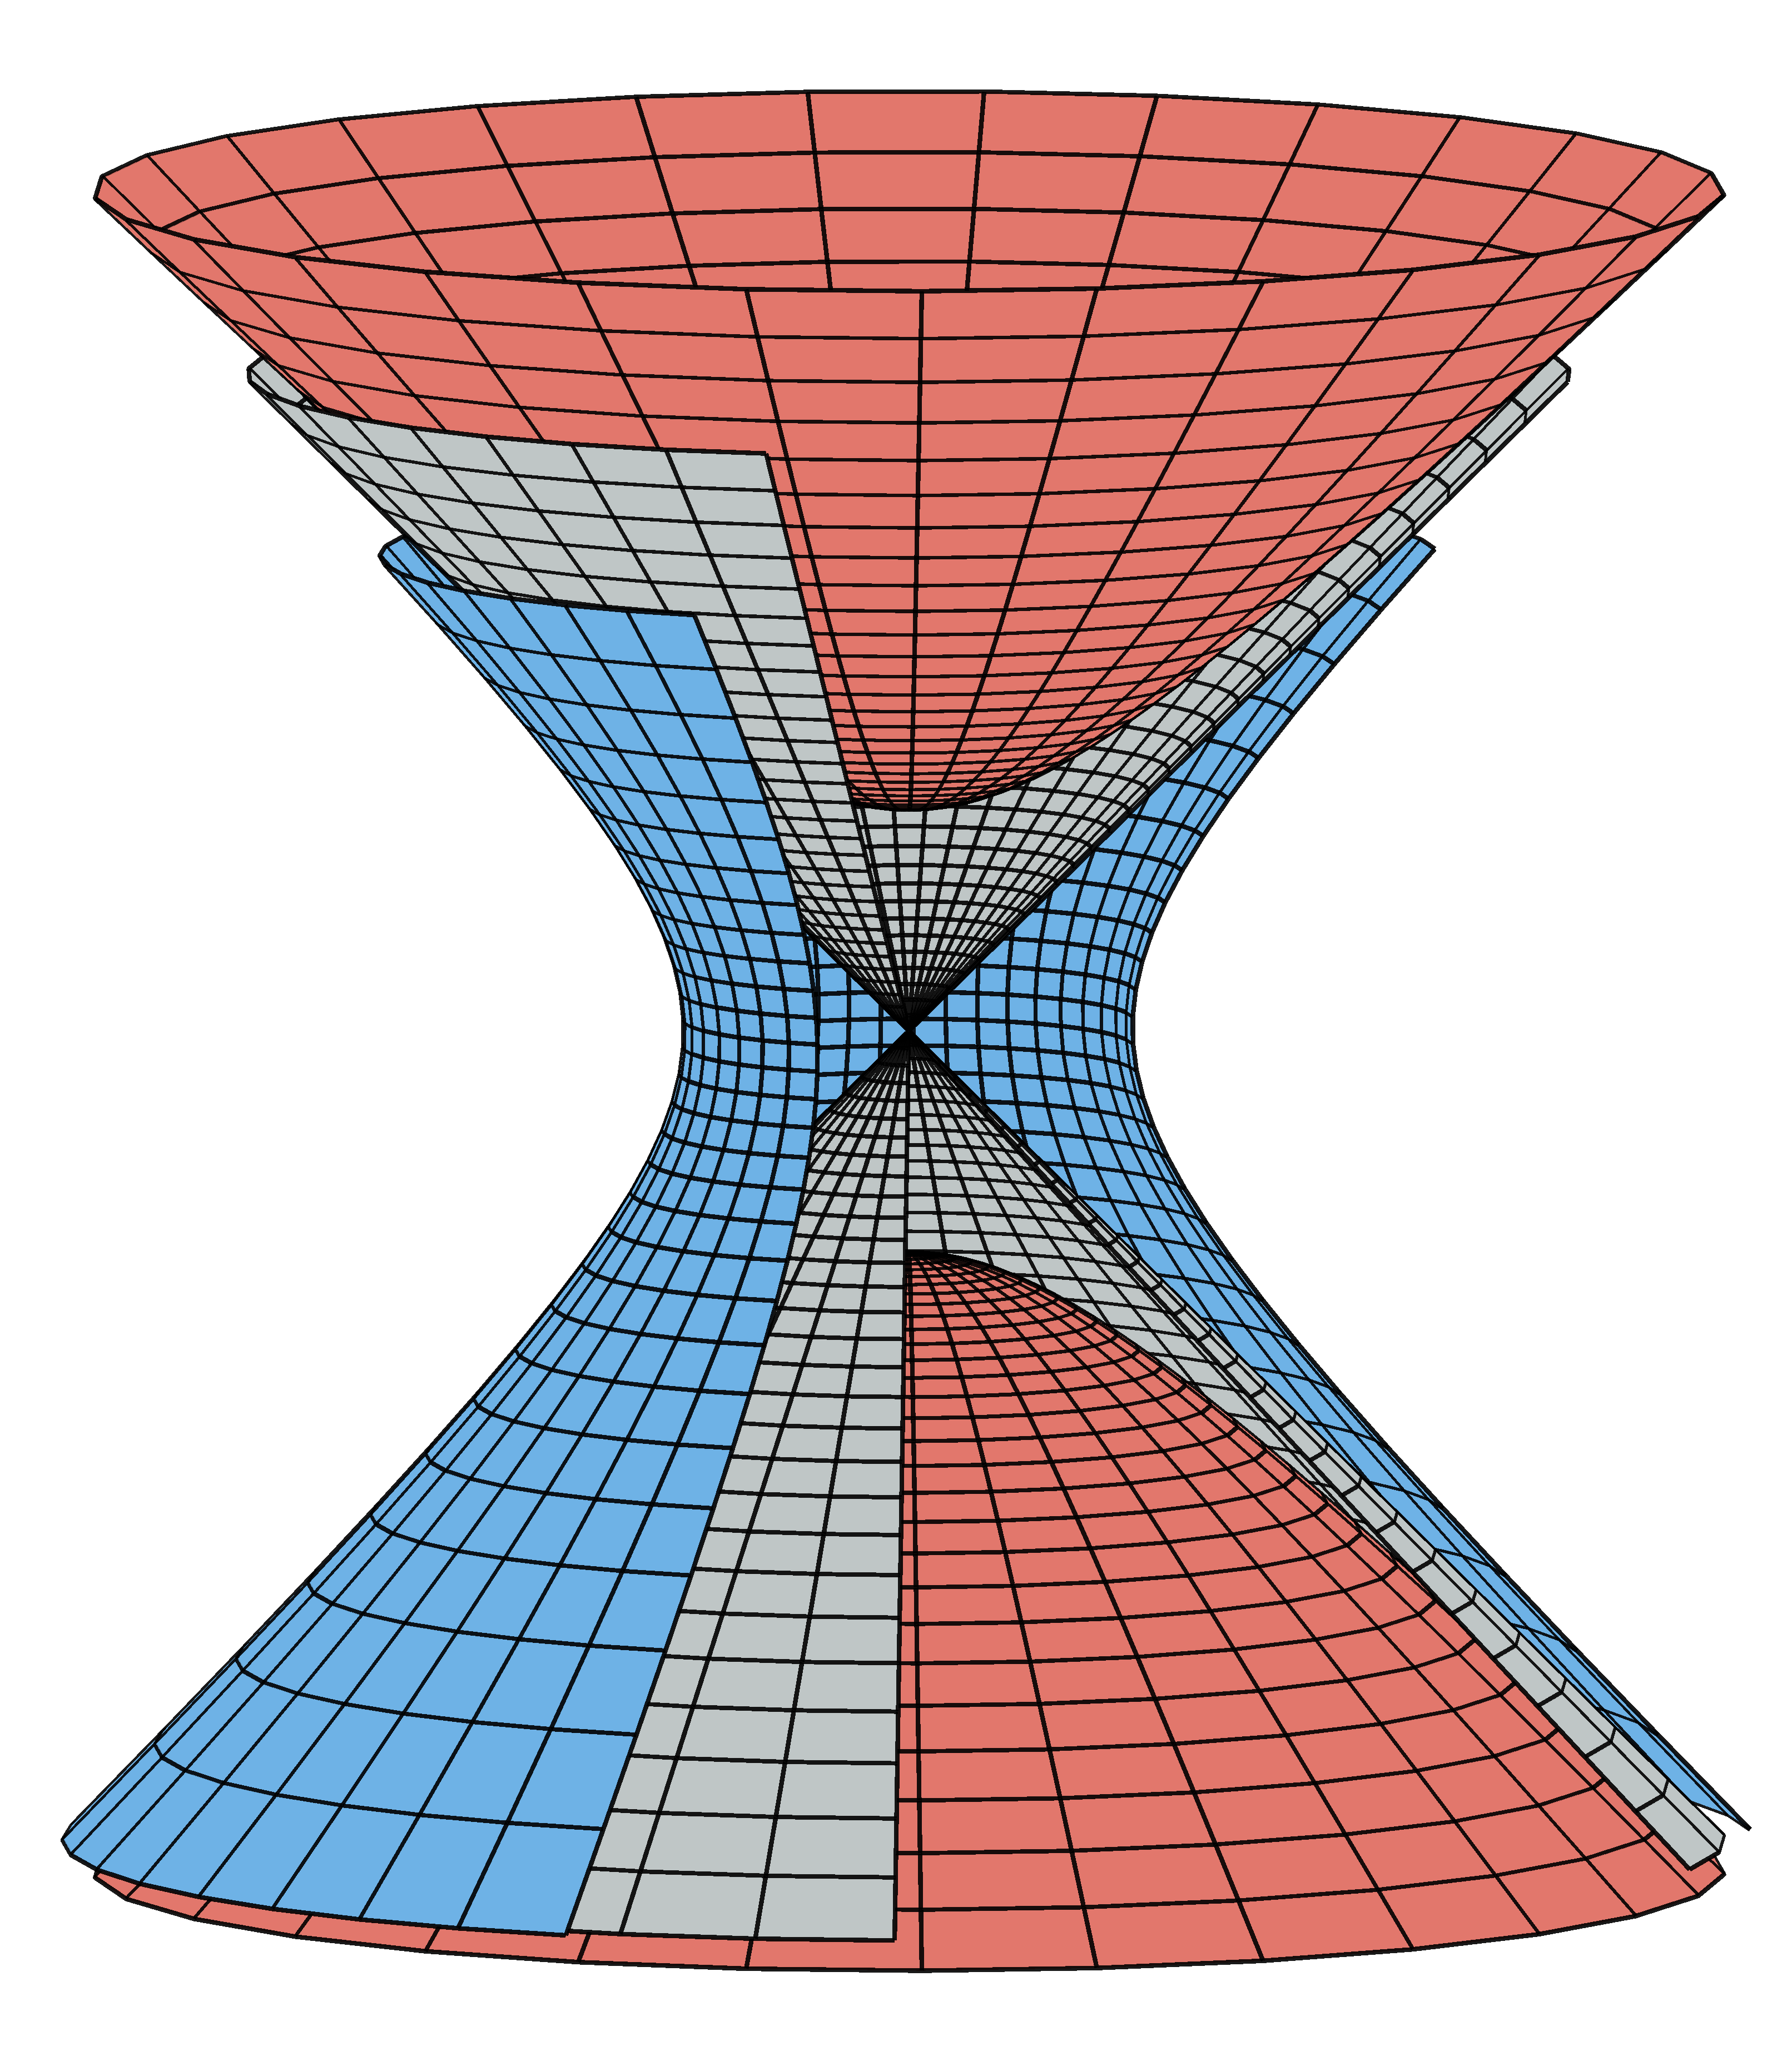
\includegraphics[]{media/other/lorentz_space.png}
    \caption{The three surfaces in Lorentzian 3-space which are }
    \label{fig:hyperboloids}
\end{figure}

Given the regime of the mechanical systems, the eigenvectors of the state transition matrix determine the particular shape of the trajectories in the phase plane. We distinguish three types of shapes:
\begin{itemize}
    \item[\circled{1}] Saddle point: two directions
    \item[\circled{2}] Stable line: two direction (?)
    \item[\circled{3}] Pure translation: translation direction?
    \item[\circled{4}] Node: two directions
    \item[\circled{6}] A center/spiral, which has elliptic trajectories. These also include the spiral nodes, since the scalar part (contraction) is not part of the vector. We can characterize the shape of the elliptic trajectories by the \emph{eccentricity} and their \emph{tilt} (i.e. the rotation of the major axes of the ellipse with respect to the phase plane axes). 
\end{itemize}

Compute real eigenvectors by substituting the action of multiplying with a vector \emph{in} the split-quaternion and solving appropriately.

\subsubsection{Underdamped systems}

\FloatBarrier
\section{Notes}
! orthogonal refers to `regular' orthogonal, Lorentz-orthogonal makes the distinction.

Motivation: $\vec{u}$ seems to be `aligned' with major direction of the elliptic trajectory in the Lorentz-orthogonal subspace, generated by the action of its cross-product. Show this formally by making use of the eigenvectors.

The basis vectors $ \qty{\vec{e}_2, \vec{e}_3}$, where $\vec{e}_2$ is the orthogonal projection of the vector $\vec{e}_1 = \uvec{u}$ on its Lorentz-orthogonal subspace, and $\vec{e}_3 \triangleq \lorcrossp{\vec{e}_1}{\vec{e}_2}$, form the real and imaginary parts of two of the eigenvectors of the matrix $\mat{U}_{\lorcrossp{}{}}$. 

Because the basis vectors $\vec{e}_2$ and $\vec{e}_3$ are also orthogonal in the Euclidean sense, the 

\begin{proof}
    Let $\uvec{u} = u_1\uvec{i} + u_2\uvec{j} + u_3\uvec{k}$. A normal vector to the Lorentz-orthogonal subspace is $
    \uvec{n} = u_1\uvec{i} - u_2\uvec{j} - u_3\uvec{k}$. Then, the basis vectors are
    \begin{equation}
        \begin{split}
            \vec{e}_2 &= 
            \uvec{u} - \frac{ \inner{\uvec{u}}{\uvec{n}} }{ \inner{\uvec{n}}{\uvec{n}} } \uvec{n} \\
            \vec{e}_3 &= \lorcrossp{\uvec{u}}{\vec{e}_2} = -\frac{ \inner{\uvec{u}}{\uvec{n}} }{ \inner{\uvec{n}}{\uvec{n}} } \qty(\lorcrossp{\uvec{u}}{\uvec{n}}),
        \end{split}
    \end{equation}
    because the Lorentz-cross product distributes over addition and $\lorcrossp{\uvec{u}}{\uvec{u}} = \vec{0}$. The proposition above claims that $\vec{e}_2 + \ii\vec{e}_3$ is an eigenvector of the matrix $\mat{U}_{\lorcrossp{}{}}$. Hence, it must be the case that $\mat{U}_{\lorcrossp{}{}}(\vec{e}_2 + \ii\vec{e}_3) = \lambda(\vec{e}_2 + \ii\vec{e}_3)$, where $\lambda$ is then an eigenvalue of the matrix. This can be verified by replacing the action of $\mat{U}_{\lorcrossp{}{}}$ with the cross product. Plugging in the definition and exploiting the linearity of the Lorentz cross-product, we obtain:
    \begin{equation*}
        \begin{split}
            \lorcrossp{\uvec{u}}{\qty(\vec{e}_2 + \ii\vec{e}_3)} 
            &= \lorcrossp{\uvec{u}}{\vec{e}_2} +
        \ii\qty(\lorcrossp{\uvec{u}}{\vec{e}_3}) \\
            &= \vec{e}_3 + \qty(\lorcrossp{\uvec{u}}{\vec{e}_3})\ii \\ 
            &=\vec{e}_3 +  \qty(\lorcrossp{\uvec{u}}{\qty(\lorcrossp{\uvec{u}}{\vec{e}_2})})\ii \\
            &=\vec{e}_3 -  \frac{ \inner{\uvec{u}}{\uvec{n}} }{ \inner{\uvec{n}}{\uvec{n}} }\qty(\lorcrossp{\uvec{u}}{\qty(\lorcrossp{\uvec{u}}{\uvec{n}})})\ii.  \\
        \end{split}
    \end{equation*}
The triple cross-product expansion, or `Lagrange formula', relates the regular cross product to the corresponding dot product:
    $$ \vec{a}\times\qty(\vec{b}\times\vec{c}) = \vec{b}\:\inner{\vec{c}}{\vec{a}} - \vec{c}\:\inner{\vec{a}}{\vec{b}}. $$
This well-known identity generalizes (easily verified) to the Lorentzian counterpart of the cross- and inner products:
    $$ 
        \lorcrossp{\vec{a}}{\qty(\lorcrossp{\vec{b}}{\vec{c}})} 
       = \vec{b}\:\lorinner{\vec{c}}{\vec{a}} - \vec{c}\:\lorinner{\vec{a}}{\vec{b}}. 
    $$
Using the Lagrange formula, the above expression becomes
    \begin{equation*}
        \begin{split}
            & \vec{e}_3 - \frac{ \inner{\uvec{u}}{\uvec{n}} }{ \inner{\uvec{n}}{\uvec{n}} }\qty(\uvec{u}\,\lorinner{\uvec{u}}{\uvec{n}} - \uvec{n}\lorinner{\uvec{u}}{\uvec{u}})\ii \\
            & =\, \vec{e}_3 - \qty(\uvec{u}\,\frac{ \lorinner{\uvec{u}}{\uvec{n}} \, \inner{\uvec{u}}{\uvec{n}} }{ \inner{\uvec{n}}{\uvec{n}} } - \uvec{n}\frac{ \inner{\uvec{u}}{\uvec{n}} }{ \inner{\uvec{n}}{\uvec{n}} })\ii \\
            & =\, \vec{e}_3 - \qty(\uvec{u} - \uvec{n}\frac{ \inner{\uvec{u}}{\uvec{n}} }{ \inner{\uvec{n}}{\uvec{n}} })\ii \\
            & =\, \vec{e}_3 - \vec{e}_2\ii. 
        \end{split}
    \end{equation*}
    The latter is the scalar multiple of the vector $\vec{e}_2 + \vec{e}_3$ by $-\ii$ - hence, this is indeed an eigenvector of the corresponding matrix.
\end{proof}
Because $\vec{e}_2$ and $\vec{e}_3$ are also orthogonal in the normal sense, they are aligned with the major axes of the elliptic trajectories generated by the cross product. Hence, they can be used to find a basis of the invariant subspace which makes the trajectories identical to those in the phase plane.


